% Retoca las líneas marcadas con TODO según las necesidades

\documentclass[oneside,a4paper,12pt]{book} % TODO: cambia "oneside" por "twoside" a la hora de imprimirlo

\usepackage[spanish]{babel}
\usepackage[utf8]{inputenc}
\usepackage{geometry}
\usepackage{makeidx}
\usepackage{url}
\usepackage{graphicx}
\usepackage{color}
\usepackage{caption}
\usepackage{acronym}
\usepackage{hyphenat}
\usepackage{a4wide}
\usepackage[normalsize]{subfigure}
\usepackage{float}
\usepackage{titlesec}
\usepackage[Lenny]{fncychap}
\usepackage{listings} % para poder hacer uso de "listings" propios (p.ej. códigos)
\usepackage{eurosym} % para poder usar el símbolo del euro con \euro {xx}
\usepackage{hyperref} % TODO: añade la opción hidelinks para imprimirlo (los enlaces no aparecerán resaltados)
\usepackage{tikz}
\usetikzlibrary{positioning, shapes}
\usepackage{multirow}
\usepackage{amsmath}
\usepackage{xcolor}  % Add this line to use colors
\usepackage{physics}
\usepackage{mdframed}



% Para que no parta las palabras
\pretolerance=10000

\setlength{\parskip}{5pt}

\newcommand{\bigrule}{\titlerule[0.5mm]} \titleformat{\chapter}[display] % cambiamos el formato de los capítulos
{\bfseries\Huge} % por defecto se usaron caracteres de tamaño huge en negrita
{% contenido de la etiqueta 
\titlerule % línea horizontal 
\filright % texto alineado a la derecha 
\Large\chaptertitlename\ % capítulo e índice en tamaño large
\Large % en lugar de 
\Huge \Large\thechapter} 
{0mm} % espacio mínimo entre etiqueta y cuerpo
{\filright} % texto del cuerpo alineado a la derecha
[\vspace{0.5mm} \bigrule] % después del cuerpo, dejar espacio vertical y trazar línea horizontal gruesa
\geometry{a4paper, left=3.5cm, right=2cm, top=3cm, bottom=2cm, headsep=1.5cm}

% Estilos para ilustrar códigos:
\definecolor{code_green}{rgb}{0,0.6,0}
\definecolor{code_gray}{rgb}{0.5,0.5,0.5}
\definecolor{code_mauve}{rgb}{0.58,0,0.82}

\lstset{frame=tb,
  language=C,
  aboveskip=3mm,
  belowskip=3mm,
  showstringspaces=false,
  columns=flexible,
  basicstyle={\small\ttfamily},
  numbers=none,
  numberstyle=\tiny\color{code_gray},
  keywordstyle=\color{blue},
  commentstyle=\color{code_green},
  stringstyle=\color{code_mauve},
  breaklines=true,
  breakatwhitespace=true,
  tabsize=3
}

\lstset{frame=tb,
  language=C++,
  aboveskip=3mm,
  belowskip=3mm,
  showstringspaces=false,
  columns=flexible,
  basicstyle={\small\ttfamily},
  numbers=none,
  numberstyle=\tiny\color{code_gray},
  keywordstyle=\color{blue},
  commentstyle=\color{code_green},
  stringstyle=\color{code_mauve},
  breaklines=true,
  breakatwhitespace=true,
  tabsize=3
}

\lstset{frame=tb,
  language=Python,
  aboveskip=3mm,
  belowskip=3mm,
  showstringspaces=false,
  columns=flexible,
  basicstyle={\small\ttfamily},
  numbers=none,
  numberstyle=\tiny\color{code_gray},
  keywordstyle=\color{blue},
  commentstyle=\color{code_green},
  stringstyle=\color{code_mauve},
  breaklines=true,
  breakatwhitespace=true,
  tabsize=3
}

%\lstset{
%	language=bash,              % Establecer el lenguaje como Bash
%	basicstyle=\ttfamily,   % Typewriter font for the code
%	commentstyle=\color{gray}, % Color of comments
%	keywordstyle=\color{blue},  % Color of keywords (optional)
%	stringstyle=\color{black},     % Color of strings (optional)
%	showstringspaces=false,      % Don't show spaces in strings
%	numbers=none,                % Disable line numbers
%	frame=single                 % Add a frame around the code
%}


% Definición de mis propios tipos: Códigos, Ecuaciones y Tablas
\DeclareCaptionType{code}[Código][Listado de códigos]
\DeclareCaptionType{myequation}[Ecuación][Listado de ecuaciones]

% TODO: especifica las reglas de separación que consideres. Algunos ejemplos:
\hyphenation{fuer-tes}
\hyphenation{mul-ti-ca-pa}
\hyphenation{res-pues-ta}
\hyphenation{di-fe-ren-tes}
\hyphenation{de-sa-rro-lla-dos}
\hyphenation{re-pre-sen-tan-do}

 % archivo de configuraci�n de estilo

\makeindex

\begin{document}
\baselineskip 1.35\baselineskip

\frontmatter

\thispagestyle{empty}
\vspace{2cm}

\begin{figure}[htb]
  \centerline{\resizebox{.60\textwidth}{!}{
\includegraphics{figs/logo_urjc}}}
\end{figure}

\begin{center}
  {\Large {\bf GRADO EN INGENIERÍA DE ROBÓTICA SOFTWARE}}
  \vspace{5mm}
 
  {\large {Escuela de Ingeniería de Fuenlabrada}}
  \vspace{5mm}

  {\large {Curso académico 2024-2025}}

  \vspace{1cm}

  {\large {\bf Trabajo Fin de Grado}}

  \vspace{2cm}

  {\Large {Robot de bajo coste para el mantenimiento de carreteras\\}}

  \vspace{5cm}
  {\bf Tutor}: Julio Vega Pérez \\
  {\bf Autor}: Julia López Augusto
\end{center}

\clearpage
\thispagestyle{empty}


% Este diseño se corresponde con la licencia CC-BY-NC-SA.
% Por supuesto, puedes poner la licencia que mejor se adapte al propósito de tu trabajo.
% Recuerda que, si no se especifica ninguna licencia, esta -como cualquier creación artística- pasaría a estar licenciada con todos los derechos reservados (copyright).

\cleardoublepage

\begin{figure}
 \ \ \ \ 
\includegraphics[width=0.25\linewidth]{figs/by-nc-sa.png}
 \label{fig:cc} 
 \end{figure}

\

\

\

\noindent
Este trabajo se distribuye bajo los términos de la licencia internacional \href{http://creativecommons.org/licenses/by-nc-sa/4.0/}{CC BY-NC-SA International License} (Creative Commons AttributionNonCommercial-ShareAlike 4.0). Usted es libre de \textit{(a) compartir}: copiar y redistribuir el material en cualquier medio o formato; y \textit{(b) adaptar}: remezclar, transformar y crear a partir del material. El licenciador no puede revocar estas libertades mientras cumpla con los términos de la licencia:

\begin{itemize}
\item \textit{Atribución}. Usted debe dar crédito de manera adecuada, brindar un enlace a la licencia, e indicar si se han realizado cambios. Puede hacerlo en cualquier forma razonable, pero no de forma tal que sugiera que usted o su uso tienen el apoyo de la licenciante.
\item \textit{No comercial}. Usted no puede hacer uso del material con propósitos comerciales.
\item \textit{Compartir igual}. Si remezcla, transforma o crea a partir del material, debe distribuir su contribución bajo la la misma licencia del original.
\end{itemize}

\begin{flushright}
		\vspace{7.0 cm}
		\emph{Documento de} \textbf{Julia López Augusto}. % TODO: pon aquí tu nombre cuando hagas el documento
\end{flushright}



\cleardoublepage

\chapter*{Agradecimientos}

Primero de todo me gustaría agradecer a mi tutor Julio toda la confianza y el apoyo depositado para poder hacer posible este proyecto. Sin ti nada de esto hubiera sido posible.\\

También agradecer a todos los profesores que he tenido a lo largo de la carrera lo importante que habéis sido para mí tanto en mi crecimiento académico, profesional como personal. Gracias a vosotros me habéis hecho ingeniera. \\

Otras personas que han sido, son y serán fundamentales en mi vida son mis padres; a los cuáles estaré eternamente agradecida por no soltarme nunca de la mano y darme todas las herramientas que han hecho posible ser quien soy hoy en día. Os quiero muchísimo.\\

Una persona que apareció en mi vida hace ya unos 7 años fue Fran, quien trajo luz en medio de tanta oscuridad y ha sido el mejor acompañante, amigo y amante de cada aventura que se presenta en la vida. Te amo con todo mi corazón y gracias de verdad por todo, ya lo sabes.\\

Los abuelos deberían ser eternos pero desgraciadamente en mi caso marcharon mucho antes de lo debido. Sé que les encantaría ver a su nieta graduada como ingeniera y me encantaría poder darles un abrazo muy fuerte y poder celebrarlo juntos pero bueno, se que allá donde estéis estaréis muy orgullosos mí tanto como yo os echo de menos a vosotros. Gracias por los años que pude conoceros y disfrutaros, quedarán para siempre en mi retina. \\

Los amigos son la familia que uno puede elegir y hoy en día puedo estar muy orgullosa y agradecida de la gente que tengo a mi lado. Gracias a Jimena, Elisa, Sofía, Maryu, Santi, Gonzalo y Álvaro por ser tan maravillosos y por estar ahí estos 4 años de alegrías, lloros, mucho trabajo y dolores de cabeza; sois increíbles.
\\
\ % Algo de separación...

\

\

\

\

\begin{flushright}
		\vspace{4.0 cm}
		\emph{A mi misma;\\
      por nunca tirar de la toalla}\\
		\par
		\vspace{1.0 cm}
		Chozas de Canales, 4 de Junio de 2024\\ %\today
		\emph{Julia López Augusto}
\end{flushright}

\thispagestyle{empty}



\cleardoublepage

\chapter*{Resumen\markboth{Resumen}{Resumen}}

% Un primer párrafo para dar contexto sobre la temática que rodea al trabajo.
La robótica es el campo de la ingeniería que se enfoca en el diseño, la construcción y la programación de robots. De todos los tipos de robots que existen cabe destacar los robots de campo que son capaces de operar en entornos no estructurados y difíciles, pero estos son de elevado coste. Es por ello que, bajo el prisma de la robótica \textit{low cost}, campo creado para hacer robots económicos, accesibles y fáciles de producir, se puede idear una solución a este problema.

% Un segundo párrafo concretando el contexto del problema abordado.
%Las carreteras son una de las infraestructuras que necesitan un constante mantenimiento y que ello conlleva un reto logístico y económico. Además, ese mantenimiento siempre ha dependido de un equipo de trabajadores expuestos a altos riesgos mientras realizan tareas laboriosas.

% En el tercer párrafo, comenta cómo has resuelto la problemática descrita en el anterior párrafo.
Una de las aplicaciones de los robots de campo es el mantenimiento de carreteras. El presente trabajo pretende solucionar este problema diseñando un robot de bajo coste que permita la detección de baches, almacene su localización, vía GPS, y calcule el volumen de estos. Además, se ha desarrollado toda una interfaz web, para que la persona de mantenimiento pueda gestionar el mantenimiento de forma cómoda e intuitiva.

El prototipo robótico se ha diseñado en 3D, para lo que se han empleado herramientas de \textit{software} libre. Su impresión se ha hecho en una impresora convencional y sus componentes \textit{hardware} de terceros se pueden encontrar fácilmente en cualquier tienda de electrónica. Además, se ha desarrollado una versión de este robot en simulación, al que se le ha dado soporte en ROS 2. 

Algunas de las técnicas empleadas en el robot físico para conseguir el objetivo principal, son: el aprendizaje supervisado, \ac{TPU}, filtros de imagen, el modelo pinhole, el algoritmo de la lazada, \ac{VFF}, servidores web, entre otros.

% en este cuarto párrafo, describe cómo han ido los experimentos.
Numerosos son los experimentos realizados, tanto para evaluar cada componente de forma individual, como para afinar el comportamiento completo. Uno de los comportamientos supone manejar el robot de forma teleoperada, y, el otro, que el robot se mueva de forma autónoma, usando una carretera adaptada como su entorno de operatividad.



\cleardoublepage

\chapter*{Acrónimos\markboth{Acrónimos}{Acrónimos}}

% Añade a continuación los acrónimos que uses en el documento. Algunos ejemplos:
\begin{acronym}
	\acro{SRI}{\emph{Stanford Research Institute}}
	\acro{KUKA}{\emph{Keller und Knappich Augsburg}}
	\acro{ABB}{\emph{Asea Brown Boveri}}
	\acro{BSA}{\emph{Backtracking Spiral Algorithm}}
	\acro{FLL}{\emph{First Lego League}}
	\acro{AGV}{\emph{Automatic Guided Vehicles}}
	\acro{AMR}{\emph{Autonomous Mobile Robots}}
    \acro{MITMA}{\emph{Ministerio de Transportes, Movilidad y Agenda Urbana}}
	\acro{CEDEX}{\emph{Centro de Estudios y Experimentación de Obras Públicas}}
	\acro{AEC}{\emph{Asociación Española de la Carretera}}
	\acro{ACEX}{\emph{Asociación de Empresas de Conservación y Explotación de Infraestructuras }}
	\acro{SIG}{\emph{Sistema de Información Geográfica}}
	\acro{IA}{\emph{Inteligencia Artificial}}
	\acro{GPS}{\emph{Global Positioning System}}
	\acro{DANA}{\emph{Depresión Aislada en Niveles Altos}}
	\acro{CAD}{\emph{Computer-Aided Design}}
	\acro{PDCA}{\emph{Plan Do Check Act}}
	\acro{CSI}{\emph{Camera Serial Interface}}
	\acro{UART}{\emph{Universal Asynchronous Receiver-Transmitter}}
	\acro{PWM}{\emph{Pulse Width Modulation}}
	\acro{LTS}{\emph{Long Time Support}}
	\acro{ROS}{\emph{Robot Operating System}}
	\acro{CLI}{\emph{Command Line Interface}}
	\acro{YOLO}{\emph{You Only Look Once}}
	
\end{acronym}


\cleardoublepage

\tableofcontents

\listoffigures

\listofcodes

\listofmyequations

\listoftables

%\pagestyle{empty}

\cleardoublepage

 % aqu� se cargan todas las "primeras p�ginas"

% Bibliograf�a
\let\OLDthebibliography=\thebibliography
\def\thebibliography#1{\OLDthebibliography{#1}
  \addcontentsline{toc}{chapter}{\bibname}}

\mainmatter

\setcounter{page}{1}
\chapter{Introducción}
\label{cap:capitulo1}
\setcounter{page}{1}

\begin{flushright}
\begin{minipage}[]{10cm}
\emph{La motivación nos impulsa a comenzar y el hábito nos permite continuar}\\
\end{minipage}\\

Jim Ryun\\
\end{flushright}

\vspace{1cm}

La robótica ha sufrido una transformación enorme a lo largo de su historia, aunque siempre teniendo en mente el mismo objetivo: cumplir con el deseo humano. Debido a esa transformación y ese deseo se ha podido consolidar este campo en la actualidad, que abarca cada sector que se pueda imaginar. Otra vertiente que ha destacado en la robótica estos últimos años ha sido la creación de robots de bajo coste para que puedan llegar a un mayor número de personas y se puedan beneficiar de esta ciencia. 

En el presente capítulo se va a abordar el contexto de la robótica, explicando brevemente su historia para poder entender realmente qué es la robótica y lo que es un robot. También se van a encuadrar los tipos de robots que existen y sus múltiples aplicaciones. Todo esto nos ayudará a poder entender mejor dónde se encuadra el presente trabajo, proporcionando los conocimientos necesarios, tanto teóricos como prácticos, que se describirán a lo largo del documento.

\section{La robótica}
\label{sec:robotica} % etiqueta para luego referenciar esta sección

La robótica es el campo de la ingeniería que se enfoca en el diseño, la construcción y la programación de robots. Y un robot se podría definir como un sistema informático formado por sensores y actuadores imprecisos, ya que operan en el mundo real que es imperfecto también. Los robots realizan tareas repetitivas, aburridas y peligrosas, y tienen que ser sensibles al entorno. Sin embargo, no existe una definición unívoca al respecto y depende del campo y de la época de la que queramos hablar. Para poder entenderlo, se va a hacer un breve resumen sobre la historia de la robótica.

Desde la antigüedad se han desarrollado ingenios o autómatas, de los cuáles muchos de ellos tenían fines religiosos, como los mostrados en la Figura \ref{fig:ancientrel}. 


\begin{figure}[ht!]
	\centering
	\begin{minipage}{0.4\linewidth}
		\centering
		\includegraphics[width=\linewidth]{figs/memnon.jpeg}
		\caption*{\centering Estatuas de Memnon $^{\ref{note:enlace1}}$} %\cite{memnon_image}
	\end{minipage}
	\hspace{2cm}
	% aquí incluir iamgen de Guerrero de terracota
	\begin{minipage}{0.35\linewidth}
		\centering
		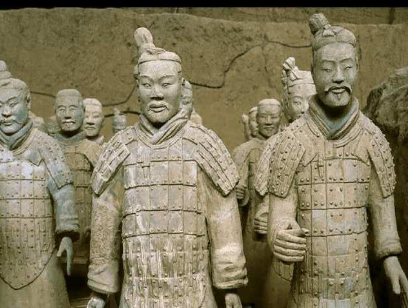
\includegraphics[width=\linewidth]{figs/terracota.png}
		\caption*{\centering Guerreros de Terracota $^{\ref{note:enlace2}}$} %\cite{gomezguerreros}
	\end{minipage}
	\caption{Ingenios de la antigüedad con fines religiosos}
	\label{fig:ancientrel}
\end{figure}


% Definir la primera nota al pie con el número 1
\setcounter{footnote}{1} % Reiniciar la numeración de notas al pie
\footnotetext[\value{footnote}]{\url{https://es.wikipedia.org/wiki/Colosos_de_Memn\%C3\%B3n}\label{note:enlace1}}

\setcounter{footnote}{2} % Reiniciar la numeración de notas al pie
\footnotetext[\value{footnote}]{\url{https://es.wikipedia.org/wiki/Guerreros_de_terracota}\label{note:enlace2}}
 
Otras invenciones que destacaban por otras aplicaciones fueron el tornillo de Arquímedes de Siracusa, la eolípila de Herón de Alejandría, el ornitóptero de Leonardo Da Vinci y el hombre de palo de Juanelo Turriano, entre otras.

En \cite{cuenca2023diseno} se trata el principio de generación hidroeléctrica, tomando en cuenta el modelo tornillo de Arquímedes. También en el artículo \cite{giri2020maquinas} se traza una línea histórica de las máquinas térmicas, teniendo en cuenta a la eolípila. Dichas invenciones aparecen reflejadas en la Figura \ref{fig:ancient}.

\begin{figure}[ht!]
	\centering
	% Imagen del tornillo de Arquímedes de Siracusa
	\begin{minipage}{0.3\linewidth}
		\centering
		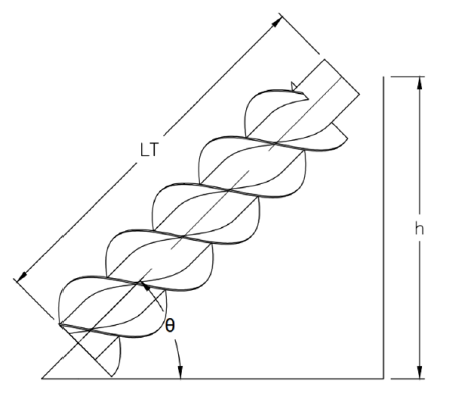
\includegraphics[width=\linewidth]{figs/arquimedes.png}
		\caption*{\centering Tornillo de Arquímedes}  %\cite{cuenca2023diseno}
	\end{minipage}
	\hspace{3cm}
	% Imagen de la eolípila
	\begin{minipage}{0.3\linewidth}
		\centering
		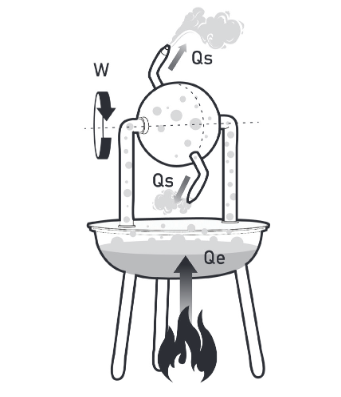
\includegraphics[width=\linewidth]{figs/eolipila.png}
		\caption*{\centering Eolípila} %\cite{giri2020maquinas}
	\end{minipage}
	%\hspace{3cm}
	% Imgen del ornitóptero
	%\begin{minipage}{0.3\linewidth}
	%	\centering
	%	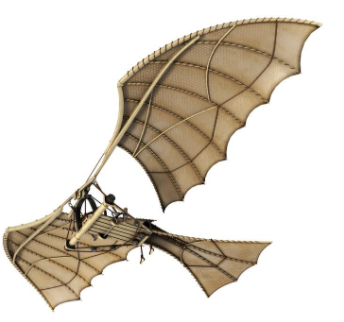
\includegraphics[width=\linewidth]{figs/davinci.png}
	%	\caption*{\centering Ornitóptero \cite{velazquezcual}}
	%\end{minipage}
	%\hspace{3cm}
	% Imagen del hombre de palo 
	%\begin{minipage}{0.3\linewidth}
	%	\centering
	%	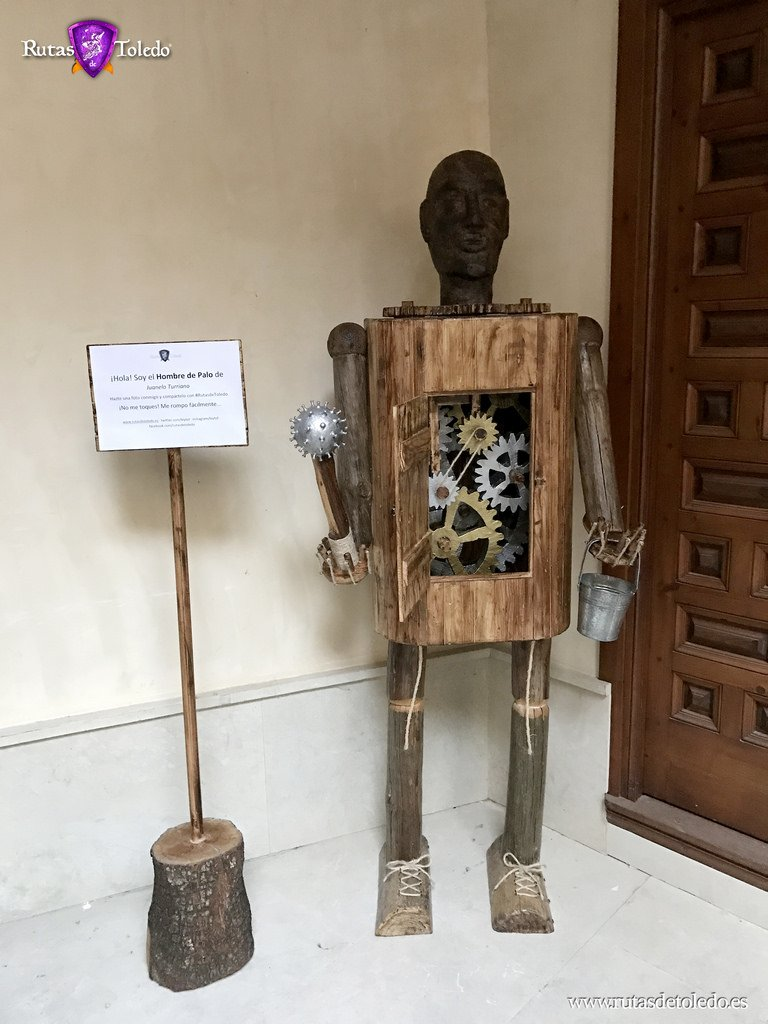
\includegraphics[width=\linewidth]{figs/hombre-palo.jpg}
	%	\caption*{\centering Hombre de palo \cite{hombredepalo_leyendasdetoledo}}
	%\end{minipage}
	\caption{Ingenios de la antigüedad con fines no religiosos}
    \label{fig:ancient}
    \end{figure}

Durante el siglo XX la ciencia dejó de ser una actividad desarrollada en aislamiento y se desarrolló en laboratorios con más gente. El movimiento del positivismo lógico fomentó las investigaciones, ya que este movimiento trataba de dar importancia a la ciencia y dejar de lado la filosofía; también, el contexto de las guerras mundiales y de las bombas nucleares influyeron significativamente en este aspecto. Ya se empieza a acuñar la palabra robot y surge Electro y Sparko de Westinghouse Electric Corporation (Figura \ref{fig:EyS}), tratado en muchas ocasiones como uno de los primeros robots, como se describe en \cite{bidaudrobots}. Un descubrimiento muy destacado fue, y sigue siendo hoy en día, la Leyes de la Robótica de Isaac Asimov, así lo transmite \cite{barcelo2004nuevo}.


\begin{figure} [h!]
	\begin{center}
		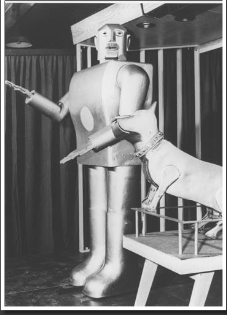
\includegraphics[width=8cm]{figs/electro-sparko.png}
	\end{center}
	\caption{Electro y Sparko} %\cite{bidaudrobots}}
	\label{fig:EyS}
\end{figure}

%\begin{figure} [h!]
%	\begin{center}
%		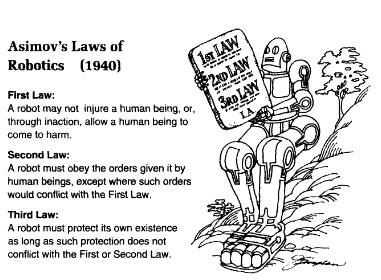
\includegraphics[width=12cm]{figs/issac-law.png}
%	\end{center}
%	\caption{ Leyes de la robótica} %\cite{barcelo2004nuevo}
%\label{fig:Asimov}
%\end{figure}


%\ac{} expande las siglas
%\acs{} no expande las siglas
\cite{nilsson1984shakey} nos cuenta que en 1969 se construye por el \ac{SRI} Internacional un prototipo experimental llamado Shakey, que era una unidad independiente de un metro y medio, equipado con dos motores, cámara de televisión y una radio conectada a un ordenador, capaz de navegar en entornos cerrados y estructurados de una forma autónoma. Sus objetivos eran aprender del medio y ser capaz de planificar trayectorias de movimiento, y las tareas que le asignaron fueron mover y detectar bloques. Sin embargo, cada movimiento podría tardar más de una hora en computarse y, aún así, podrían producirse fallos. A Shakey se le conoce como el primer robot móvil (Figura \ref{fig:sigloxx} izquierda). 

%\begin{figure} [h!]
%	\begin{center}
%		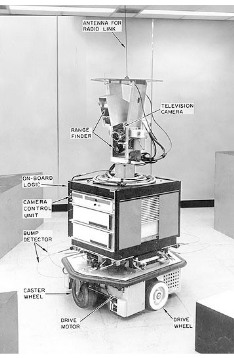
\includegraphics[width=8cm]{figs/shakey.png}
%	\end{center}
%	\caption{Robot Shakey} %\cite{nilsson1984shakey}}
%	\label{fig:shakey}
%\end{figure}


Otro robot muy conocido  y descrito en \cite{earnest2012stanfordcart} es la carreta de Stanford, que era capaz de ver y moverse en cualquier ambiente. Con la cámara que disponía, era capaz de calcular y trazar distancias. Sin embargo, tardaba cinco horas en recorrer treinta metros (Figura \ref{fig:sigloxx} derecha). 

%\begin{figure} [h!]
%	\begin{center}
%		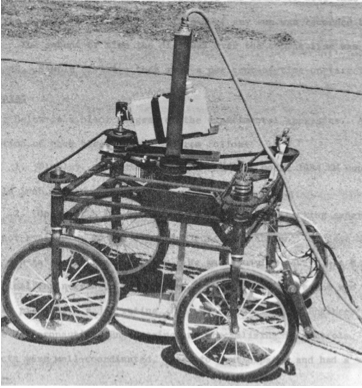
\includegraphics[width=8cm]{figs/stanford.png}
%	\end{center}
%	\caption{Carreta de Stanford}
%	\label{fig:stanford}
%\end{figure}


\begin{figure}[ht!]
	\centering
	% Imagen del tornillo de Arquímedes de Siracusa
	\begin{minipage}{0.35\linewidth}
		\centering
		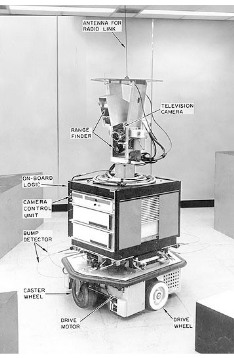
\includegraphics[width=\linewidth]{figs/shakey.png}
		\caption*{\centering Robot Shakey}  %\cite{cuenca2023diseno}
	\end{minipage}
	\hspace{2cm}
	% Imagen de la eolípila
	\begin{minipage}{0.49\linewidth}
		\centering
		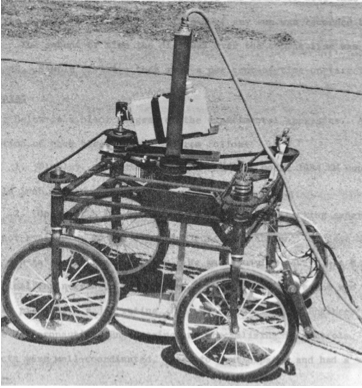
\includegraphics[width=\linewidth]{figs/stanford.png}
		\caption*{\centering Carreta de Stanford}
	\end{minipage}
	\caption{Algunos robots del siglo XX}
	\label{fig:sigloxx}
\end{figure}

Ya a partir de la década de los 80 se decidió que el acceso a los robots fuese para todo el mundo, lo que provocó asombro, inquietud y miedo, ya que el desconocimiento suele generar rechazo. El mundo de la literatura y cine tampoco ayudaba en ese aspecto, ya que se presentaba al robot como algo perjudicial para la humanidad. Afortunadamente, esta situación va menguando con el tiempo, y se está consiguiendo ver a los robots como un asistente del ser humano que lo que quiere es mejorar su calidad de vida. Las dos grandes áreas de investigación centradas en tal propósito son la robótica industrial y la robótica de servicio, que veremos detalladamente a continuación.
%Para conocer en qué ámbitos un robot puede ayudar al ser humano, es necesario conocer que se clasifican en robots industriales y de servicio.


\subsection{Robots industriales}
\label{subsec:robotindustrial}

Los robots industriales son, de forma resumida, brazos robotizados y manipuladores que tienen más de tres grados de libertad, trabajan en entornos controlados y usan efectores como: pinzas, ventosas. etc. Usan control por posición y planificación de trayectorias para poder controlar dichos brazos y poder realizar operaciones como \textit{pick and place}, ensamble de piezas, entre otros. Una variante de los robots industriales son los cobots: capaces de interactuar y colaborar con humanos como se describe en  \cite{ELZAATARI2019162} (Figura \ref{fig:robindustriales} derecha). Dentro del mercado de los robots industriales se puede ver que tiene proveedores asentados como \acs{KUKA}\footnote{\url{https://www.kuka.com/es-es}} o \acs{ABB}\footnote{\url{https://new.abb.com/es}}.



\begin{figure}[ht!]
	\centering
	\begin{minipage}{0.44\linewidth}
		\centering
		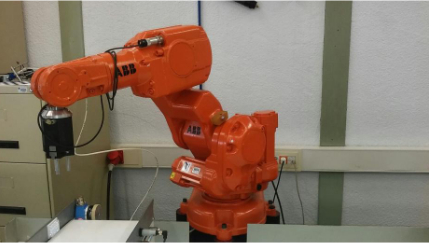
\includegraphics[width=\linewidth]{figs/brazoIRB140.png}
		\caption*{\centering Brazo robot ABB IRB 140 $^{\ref{note:enlace5}}$}

	\end{minipage}
	\hspace{1cm}
	\begin{minipage}{0.4\linewidth}
		\centering
		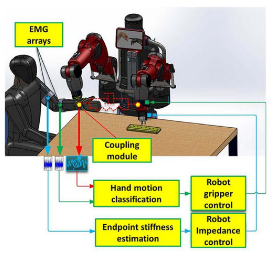
\includegraphics[width=\linewidth]{figs/cobot.png}
		\caption*{\centering Cobot}
		
	\end{minipage}
	\caption{Robots industriales}
	\label{fig:robindustriales}
\end{figure}



\setcounter{footnote}{5} % Establecer la numeración de la siguiente nota al pie
\footnotetext[\value{footnote}]{\url{https://www.youtube.com/watch?v=BBrLAOr89KY}\label{note:enlace5}}


\subsection{Robots de servicio}
\label{subsec:robotservicio}

Los robots de servicios son todos aquellos que no son industriales; por lo tanto, tienen menos de 3 grados de libertad, no trabajan en un entorno controlado, son más difíciles de programar, toman aplicaciones heterogéneas y todavía se encuentran en un mercado inmaduro. Existen muchos tipos de robots de servicio, de los cuáles a continuación se enumeran algunos campos con algunos de sus respectivos ejemplos.


\subsubsection{Robots de limpieza}
\label{subsubsec:robotlimpieza}

En \cite{plaza_robotica_servicio} se define a los robots de limpieza como aquellos robots que se encargan de eliminar la suciedad. Dependiendo de sus características, pueden ser capaces de aspirar y fregar el suelo, o de limpiar los cristales de las ventanas. Estos últimos son comunes en edificios que tienen grandes ventanales y un difícil acceso a ellos. Las aspiradoras se encuentran en un mercado mundial asentado cuyos inicios eran aspiradoras que usaban sensores de contacto, encoders y una navegación pseudoaleatoria (Figura \ref{fig:roblimpieza} izquierda), y han evolucionado hasta el punto de usar mapas para poder navegar y poder localizarse. También usan algoritmos sofisticados, como navegación de cobertura por barridos sistemáticos \acs{BSA}, y se componen de sensores más sofisticados, como láseres y cámaras, que son capaces de detectar obstáculos, como calcetines, y ser capaz de esquivarlos (Figura \ref{fig:roblimpieza} derecha).


\begin{figure}[ht!]
	\centering
	\begin{minipage}{0.3\linewidth}
		\centering
		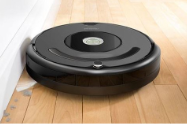
\includegraphics[width=\linewidth]{figs/gama-baja.png}
		\caption*{\centering Modelo económico }% \cite{plaza_robotica_servicio}}
	\end{minipage}
	\hspace{3cm}
	% aquí incluir iamgen de Guerrero de terracota
	\begin{minipage}{0.3\linewidth}
		\centering
		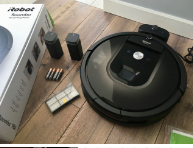
\includegraphics[width=\linewidth]{figs/gama-alta.png}
		\caption*{\centering Gama alta} % \cite{plaza_robotica_servicio}}
	\end{minipage}
	\caption{Robots de limpieza Roomba, de iRobot$^{\ref{note:enlace6}}$}
	\label{fig:roblimpieza}
\end{figure}

\setcounter{footnote}{6} % Establecer la numeración de la siguiente nota al pie
\footnotetext[\value{footnote}]{\url{https://www.irobot.es/}\label{note:enlace6}}

\subsubsection{Robots de entretenimiento}
\label{subsubsec:robotentretenimiento}

Son aquellos robots que tienen aplicaciones heterogéneas en un mercado educativo asentado, pero también existen muchos prototipos sin un uso comercial claro. En educación se ha ido introduciendo la robótica de manera muy atractiva y didáctica a los estudiantes hasta el punto de conseguir tener una asignatura destinada a la robótica y poder participar en competiciones como: \ac{FLL}\footnote{\url{https://firstlegoleague.soy/}}, Robocup Junior\footnote{\url{https://junior.robocup.org/}} y Robocampeones\footnote{\url{https://sites.google.com/view/robocampeonesfuenlabrada/}}, entre otros (Figura \ref{fig:robed} izquierda).  En dicha asignatura se adquieren conocimientos generales de programación, impresión 3D, lógica, introducción a la electrónica y los microcontroladores.

Los prototipos nombrados anteriormente suelen ser demostradores tecnológicos que se crean para exhibiciones, se encuentran a la vanguardia de la tecnología y sirven para atraer un mayor número de clientes como puede ser: Spot de Boston Dynamics, Pepper de Softbank o Sophia de Hanson Robotics. En la Figura \ref{fig:robed} (derecha) se pueden ver un ejemplo de estos demostradores.


\begin{figure}[ht!]
	\centering
	\begin{minipage}{0.35\linewidth}
		\centering
		
\includegraphics[width=\linewidth]{figs/FLL_TO19.jpg}
		\caption*{\centering \ac{FLL} Toledo $^{\ref{note:enlace10}}$}
	\end{minipage}
	\hspace{3cm}
	% aquí incluir imagen de Spot
	\begin{minipage}{0.3\linewidth}
		\centering
		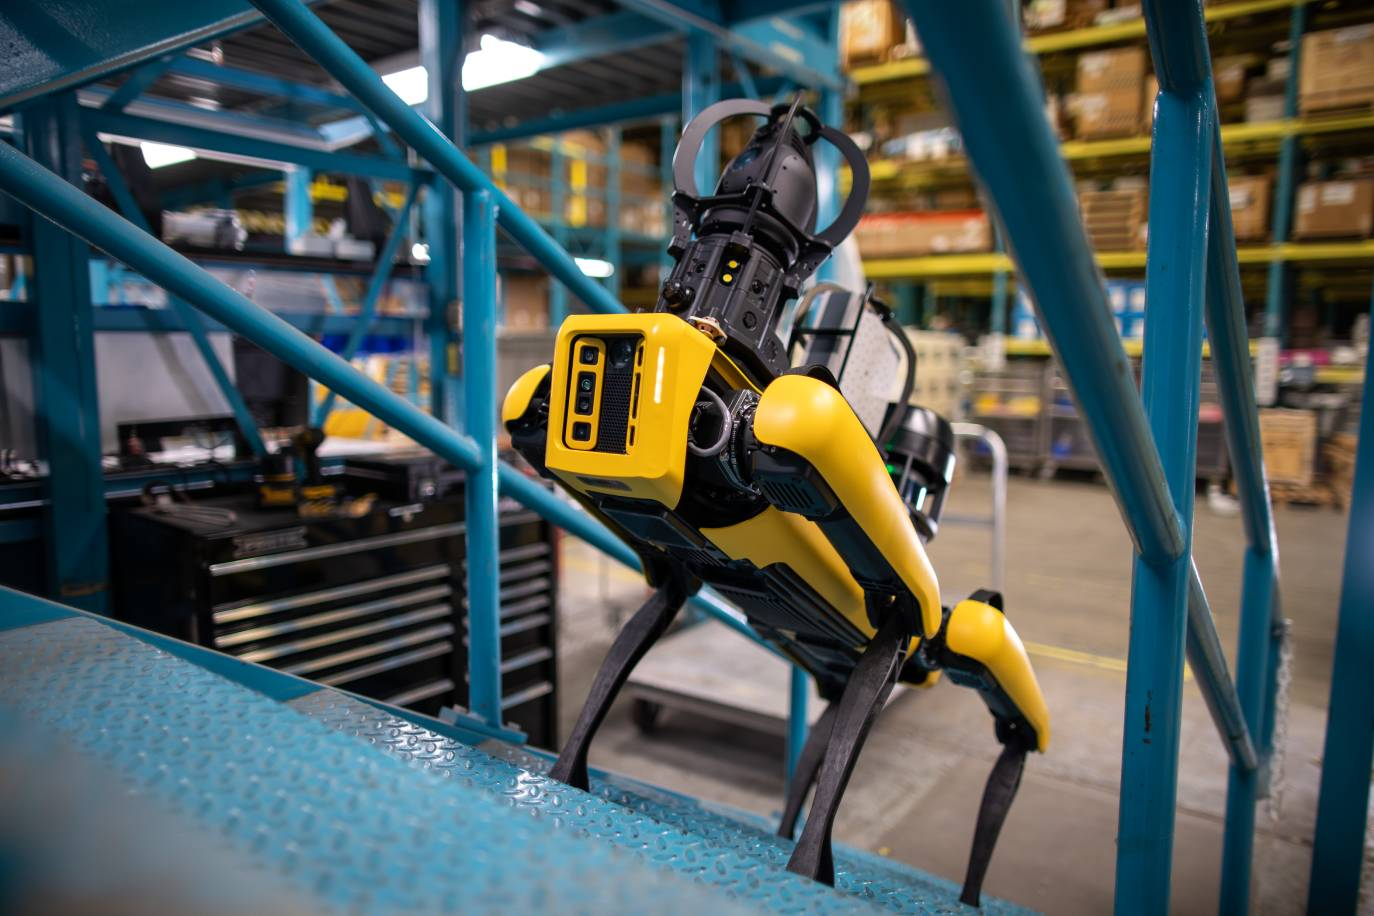
\includegraphics[width=\linewidth]{figs/spot.jpg}
		\caption*{\centering Spot de Boston Dynamics $^{\ref{note:enlace11}}$}
	\end{minipage}
	\caption{Robótica enfocada al entretenimiento}
	\label{fig:robed}
\end{figure}

\setcounter{footnote}{10} % Establecer la numeración de la siguiente nota al pie
\footnotetext[\value{footnote}]{\url{https://www.uclm.es/noticias/febrero2019/toledo/finalfirstlegoleague}\label{note:enlace10}}


\setcounter{footnote}{11} % Establecer la numeración de la siguiente nota al pie
\footnotetext[\value{footnote}]{\url{https://bostondynamics.com/products/spot/}\label{note:enlace11}}

\begin{mdframed}[backgroundcolor=yellow, linecolor=yellow]
\subsubsection{Robots de salud}
\label{subsubsec:robotsalud}


Los robots de salud sirven para mejorar la calidad de la atención médica y apoyar a los profesionales de la salud en diversas tareas. De esas tareas se pueden enumerar las siguientes: telepresencia, asistentes personales, cirugía, desinfección, esterilización, transporte interno y rehabilitación. De este gran abanico de tareas se puede destacar algunas aplicaciones que se puede ver en la Figura \ref{fig:robsalud}.
\end{mdframed}

\begin{figure}[ht!]
	\centering
	\begin{minipage}{0.5\linewidth}
		\centering
		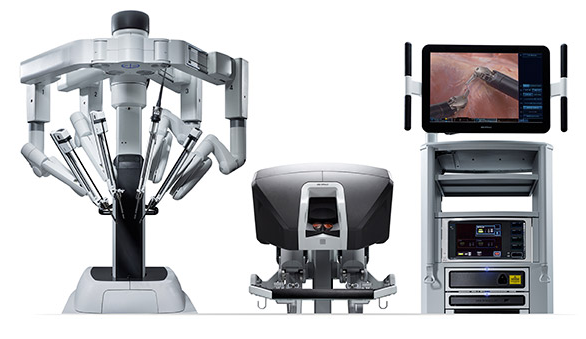
\includegraphics[width=\linewidth]{figs/davincimed.png}
		\caption*{\centering Robot Da Vinci $^{\ref{note:enlace12}}$}
	\end{minipage}
    \hspace{1 cm}
	% aquí incluir imagen de  mako
	\begin{minipage}{0.15\linewidth}
		\centering
		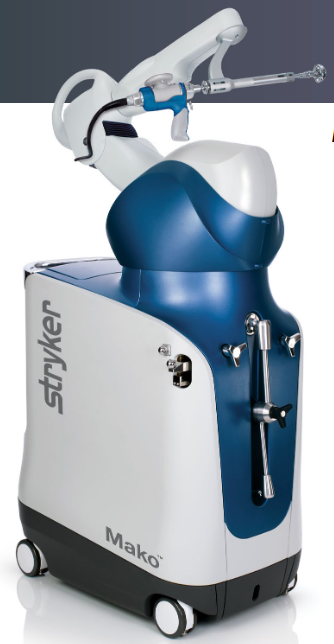
\includegraphics[width=\linewidth]{figs/mako.png}
		\caption*{\centering Robot Mako $^{\ref{note:enlace13}}$}
	\end{minipage}
    \hspace{3cm}
    \begin{minipage}{0.2\linewidth}
    	\centering
    	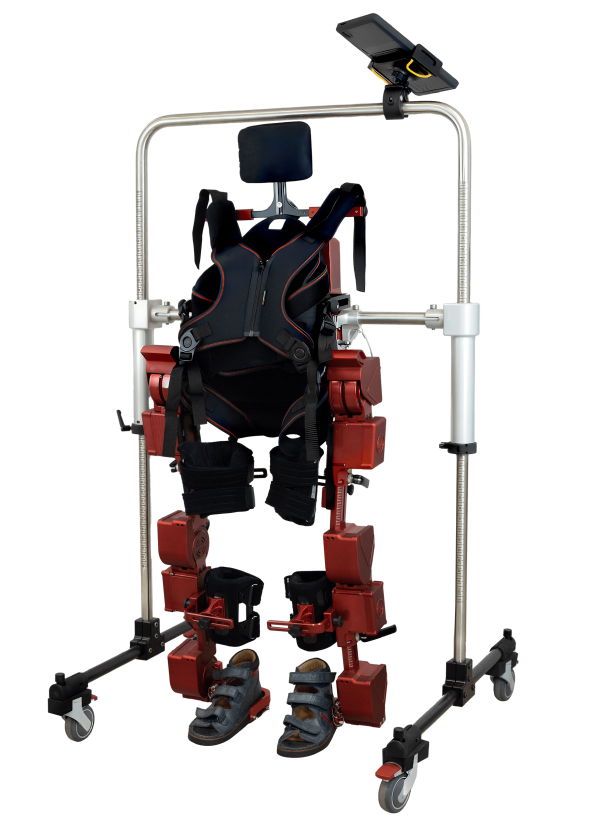
\includegraphics[width=\linewidth]{figs/marsi.png}
    	\caption*{\centering Marsi Bionics $^{\ref{note:enlace14}}$}
    \end{minipage}
    \hspace{3cm}
    \begin{minipage}{0.25\linewidth}
    	\centering
    	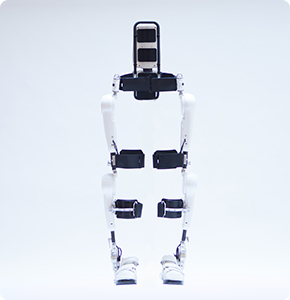
\includegraphics[width=\linewidth]{figs/cyberdyne.jpg}
    	\caption*{\centering CyberDyne $^{\ref{note:enlace15}}$}
    \end{minipage}
	\caption{Robots de salud}
	\label{fig:robsalud}
\end{figure}


\setcounter{footnote}{12} % Establecer la numeración de la siguiente nota al pie
\footnotetext[\value{footnote}]{\url{https://www.abexsl.es/es/sistema-robotico-da-vinci/que-es}\label{note:enlace12}}

\setcounter{footnote}{13} % Establecer la numeración de la siguiente nota al pie
\footnotetext[\value{footnote}]{\url{https://www.stryker.com/content/dam/stryker/joint-replacement/systems/mako-system-overview/resources}\label{note:enlace13}}

\setcounter{footnote}{14} % Establecer la numeración de la siguiente nota al pie
\footnotetext[\value{footnote}]{\url{https://www.marsibionics.com/}\label{note:enlace14}}

\setcounter{footnote}{15} % Establecer la numeración de la siguiente nota al pie
\footnotetext[\value{footnote}]{\url{https://www.cyberdyne.com/}\label{note:enlace15}}

\begin{mdframed}[backgroundcolor=yellow, linecolor=yellow]
\subsubsection{Robots de logística}
\label{subsubsec:robotlogistica}

Los robots de logística son sistemas automatizados diseñados para mejorar la eficiencia, precisión y velocidad en la gestión de la cadena de suministro y operaciones logísticas en cadenas de montaje y almacenes. Generalmente, los sistemas automatizados son flotas de robots a las que se les aplica distintas arquitecturas \textit{software} como puede ser \acs{AGV} o \acs{AMR} para poder realizar la tarea asignada. También existen prototipos de robots de reparto que son capaces de hacer entrega de última milla. La Figura \ref{fig:robreparto}  muestra ejemplos de robots de reparto. 
\end{mdframed}

\begin{figure}[ht!]
	\centering
	\begin{minipage}{0.3\linewidth}
		\centering
		\includegraphics[width=\linewidth]{figs/skypod.png}
		\caption*{\centering Skypod de Exotec $^{\ref{note:enlace16}}$ }
	\end{minipage}
	\hspace{3cm}
	% aquí incluir imagen de Amazon prime air
	\begin{minipage}{0.3\linewidth}
		\centering
		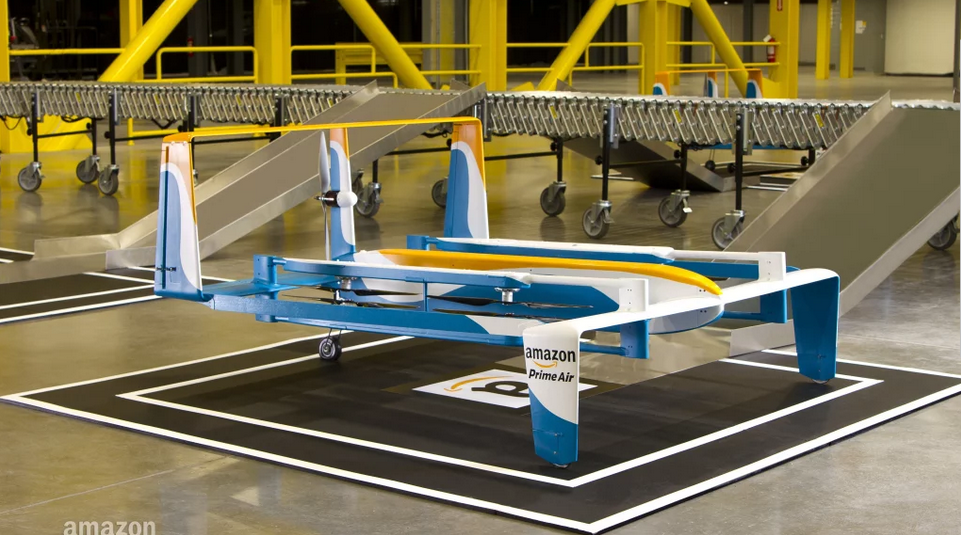
\includegraphics[width=\linewidth]{figs/amazon.png}
		\caption*{\centering Amazon Prime Air $^{\ref{note:enlace17}}$}
	\end{minipage}
	\caption{Robots de logística}
	\label{fig:robreparto}
\end{figure}

\setcounter{footnote}{16} % Establecer la numeración de la siguiente nota al pie
\footnotetext[\value{footnote}]{\url{https://exotecbydexter.com/skypod/}\label{note:enlace16}}


\setcounter{footnote}{17} % Establecer la numeración de la siguiente nota al pie
\footnotetext[\value{footnote}]{\url{https://www.aboutamazon.es/noticias/innovacion/prime-air}\label{note:enlace17}}

\section{Robots de campo}
\label{sec:robotcampo}

En \cite{thorpe2003field} se define a los robots de campo como la automatización de muchas plataformas terrestres, marítimas y aéreas en aplicaciones como la minería, la manipulación de carga, la agricultura, la exploración y explotación submarina, las carreteras, la exploración planetaria, la vigilancia costera y el rescate, entre otros. La robótica de campo se caracteriza por la aplicación de los principios robóticos más avanzados en cuanto a sensado, control y razonamiento en entornos no estructurados y difíciles. El atractivo de la robótica de campo es que es una ciencia desafiante, involucra los últimos principios de ingeniería y diseño de sistemas, y ofrece la verdadera posibilidad de que los principios robóticos hagan una contribución económica y social sustancial en muchas áreas de aplicación diferentes. En general, los robots de campo son plataformas móviles que trabajan al aire libre, a menudo produciendo interacciones fuertes con sus entornos, sin supervisión humana.

En los últimos años se ha podido notar un gran progreso en el desarrollo y la implementación de sistemas robóticos de campo. En la Figura \ref{fig:robcampo} se pueden ver ejemplos al respecto. Por contra, debido a las condiciones que se tienen que someter estos robots, su coste es elevado e imposibilita que su uso se pueda extender a aquellos lugares que necesiten de su servicio y que tienen bajos recursos. Es por esto que existe la creciente necesidad de que, para ciertas aplicaciones que no tienen condiciones tan extremas, se creen robots asequibles que puedan lidiar con determinadas tareas. A continuación veremos este campo de investigación. 


\begin{figure}[ht!]
	\centering
	\begin{minipage}{0.3\linewidth}
		\centering
		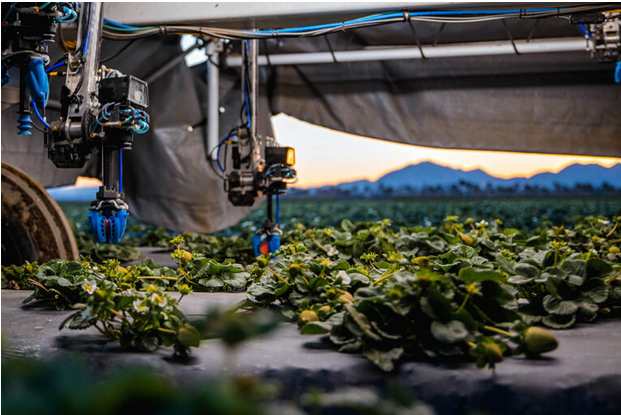
\includegraphics[width=\linewidth]{figs/strawberry.png}
		\caption*{\centering TX Robotic Strawberry Harvester $^{\ref{note:enlace18}}$ }
	\end{minipage}
	\hspace{3 cm}
	% aquí incluir imagen de  mako
	\begin{minipage}{0.3\linewidth}
		\centering
		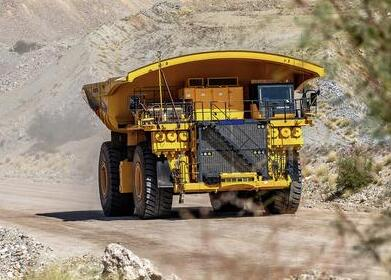
\includegraphics[width=\linewidth]{figs/komatsu.jpeg}
		\caption*{\centering FrontRunner Autonomous Haulage System (AHS) $^{\ref{note:enlace19}}$ }
	\end{minipage}
	\hspace{3cm}
	\begin{minipage}{0.3\linewidth}
		\centering
		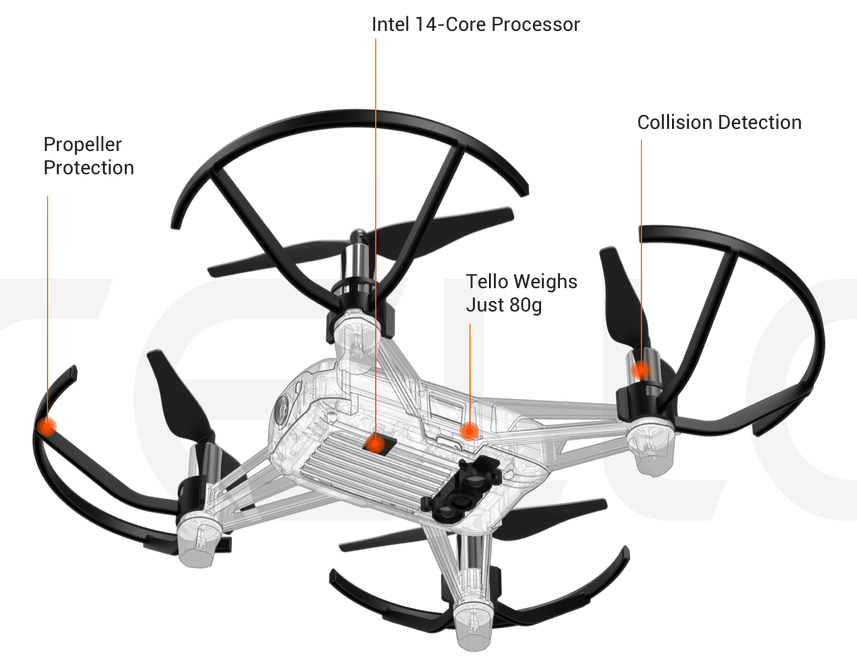
\includegraphics[width=\linewidth]{figs/tello.png}
		\caption*{\centering Drone Tello $^{\ref{note:enlace20}}$ }
	\end{minipage}
	\hspace{3cm}
	\begin{minipage}{0.3\linewidth}
		\centering
		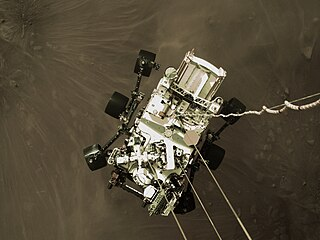
\includegraphics[width=\linewidth]{figs/perseverance.jpg}
		\caption*{\centering Perseverance $^{\ref{note:enlace21}}$ }
	\end{minipage}
	\caption{Robots de campo}
	\label{fig:robcampo}
\end{figure}


\setcounter{footnote}{18} % Establecer la numeración de la siguiente nota al pie
\footnotetext[\value{footnote}]{\url{https://advanced.farm/technology/strawberry-harvester/}\label{note:enlace18}}
\setcounter{footnote}{19} % Establecer la numeración de la siguiente nota al pie
\footnotetext[\value{footnote}]{\url{https://www.komatsu.com/en/technology/smart-mining/loading-and-haulage/autonomous-haulage-system/}\label{note:enlace19}}
\setcounter{footnote}{20} % Establecer la numeración de la siguiente nota al pie
\footnotetext[\value{footnote}]{\url{https://www.ryzerobotics.com/es/tello}\label{note:enlace20}}
\setcounter{footnote}{21} % Establecer la numeración de la siguiente nota al pie
\footnotetext[\value{footnote}]{\url{https://es.wikipedia.org/wiki/Perseverance}\label{note:enlace21}}


\section{Robots de bajo coste}
\label{sec:robotbajocoste}

Los robots de bajo coste son aquellos robots diseñados y fabricados con el objetivo de ser económicos, accesibles y fáciles de producir. Estos robots suelen emplear componentes menos costosos y métodos de fabricación simplificados para reducir el precio final. Algunas características clave de los robots de bajo coste incluyen:

\begin{itemize}
	\item \textit{Componentes asequibles}. Utilizan materiales de propósito general y componentes electrónicos más baratos, coordinados por alguna placa de bajo coste como Arduino o Raspberry Pi.
	\item \textit{Simplicidad en el diseño}. Tienen diseños más sencillos que han sido creados usando técnicas de diseño e impresión 3D, facilitando su actualización y mantenimiento.
	\item \textit{Accesibilidad}. Están diseñados para ser utilizados por cualquier tipo de persona, sin tener una formación avanzada de la materia.
	\item \textit{Educación y prototipos}. Ampliamente usados en educación para facilitar el aprendizaje y también en la creación de prototipos rápidos y asequibles.
	\item \textit{Versatilidad}. Se adaptan a numerosas aplicaciones, desde las más sencillas hasta proyectos más complejos.
	
\end{itemize}\


En resumen, los robots de bajo coste permiten la democratización de la tecnología robótica, facilitando su acceso a un público más amplio y fomentando la innovación y el aprendizaje en diferentes campos. En la Figura \ref{fig:roblowcost} se puede apreciar una aplicación real reciente de la robótica de bajo coste de la universidad \textit{Carnegie Mellon} descrita en el artículo \cite{shaw2024leap}.

\begin{figure} [h!]
	\begin{center}
		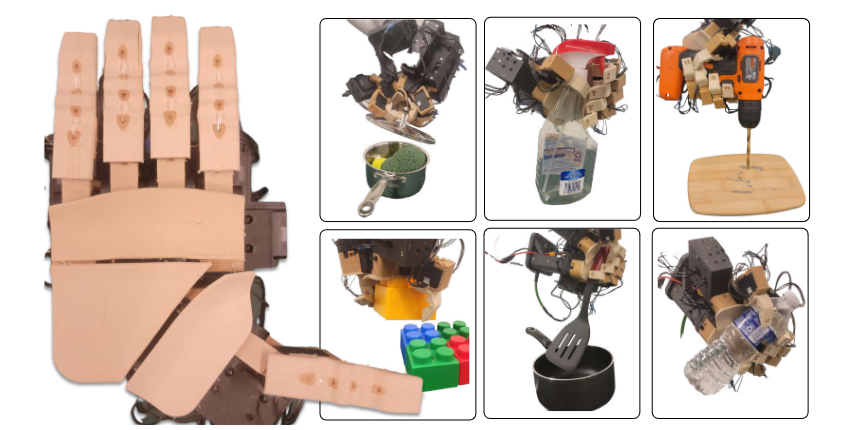
\includegraphics[width=16cm]{figs/handlowcost.png}
	\end{center}
	\caption{Mano Antropomórfica Híbrida Rígida y Suave} %\cite{shaw2024leap}}
	\label{fig:roblowcost}
\end{figure}

%Sabiendo que existen los robots de campo y la robótica de bajo coste, es necesario explorar y conocer las instituciones, los tipos de irregularidades en la carretera y los procesos actuales que existen en España para poder tener un correcto mantenimiento de ellos. 

Con esta base tecnológica, uno de los desafíos donde los robots de bajo coste están mostrando un gran potencial es en tareas repetitivas, como las tareas de mantenimiento, por ejemplo de infraestructuras como las carreteras. A medida que se buscan soluciones más eficientes y económicas para mantener y mejorar las infraestructuras, los robots de bajo coste pueden ser una pieza clave en este proceso.
%los robots de bajo coste pueden abordar problemas globales en campos que requieren soluciones económicas y eficientes, como el mantenimiento de infraestructuras públicas.

El mantenimiento de infraestructuras públicas, y en especial el de las carreteras, es una tarea de vital importancia para garantizar la seguridad y el bienestar de las personas. Sin embargo, también representa un reto logístico y económico significativo. Las carreteras, expuestas constantemente a condiciones climáticas adversas, tráfico pesado y el desgaste natural, requieren un mantenimiento constante para prevenir accidentes y asegurar la movilidad eficiente de personas y mercancías.

Tradicionalmente, este mantenimiento ha dependido de métodos manuales y laboriosos. Equipos de trabajadores inspeccionan las carreteras, identifican los daños y proceden a repararlos, lo que implica un alto coste en tiempo, recursos humanos y materiales. Además, la intervención en las carreteras conlleva cortes de tráfico que generan congestión y molestias tanto para conductores como para peatones.

Aquí es donde la tecnología de los robots de bajo coste puede ofrecer una solución disruptiva. El desarrollo de estos robots ha llegado a un punto en el que pueden ser integrados en el proceso de mantenimiento de carreteras de manera eficaz. Al ser equipados con actuadores, sensores avanzados y algoritmos de \ac{IA}, estos robots tienen la capacidad de detectar y arreglar automáticamente irregularidades en el pavimento, evaluando su tamaño y gravedad. Esta automatización permitiría realizar inspecciones más frecuentes y precisas, reduciendo el margen de error humano, facilitando intervenciones más rápidas y localizadas, y mejorando las condiciones de seguridad de los trabajadores.

La posibilidad de desplegar múltiples robots de bajo coste a lo largo de una red de carreteras también representa una ventaja significativa. Estos robots pueden realizar inspecciones de forma continua, recorriendo largas distancias y detectando problemas antes de que se conviertan en riesgos graves para la seguridad vial. Además, los robots pueden operar en entornos donde el acceso humano es complicado o peligroso, como en carreteras rurales o áreas montañosas.

En este contexto, la versatilidad y el bajo coste de los robots también resultan beneficiosos cuando se trata de reparaciones. Actualmente, las reparaciones suelen ser costosas y temporales, lo que significa que el mismo área puede requerir múltiples intervenciones a lo largo del tiempo. Sin embargo, con robots capaces de aplicar reparaciones rápidas y precisas en el lugar y momento adecuados, se podría reducir la frecuencia de intervenciones costosas y prolongar la vida útil del pavimento. 

Es por todo lo expuesto anteriormente que es necesario conocer la situación de las carreteras en España, conocer qué tipos de deterioros existen, así cómo definir en cuál de todos se va a centrar este proyecto. De este modo, se podrá implementar soluciones innovadoras, como el uso de robots de bajo coste, que no solo optimicen los recursos, sino que también mejoren la seguridad vial y la sostenibilidad del sistema de carreteras a largo plazo.


\section{Conservación de carreteras en España}
\label{sec:conservacioncarreteras}

Según informa el \ac{MITMA}\footnote{\url{https://www.transportes.gob.es/carreteras/catalogo-y-evolucion-de-la-red-de-carreteras}} la red de carreteras de España tiene, a 31 de diciembre de 2023, 165.375 kilómetros, de los cuales 26.473 km forman la \ac{RCE}, que gestiona el \acs{MITMA} y recoge el 52,5\% del tráfico total y el 64,57\% del tráfico pesado. Además, hay 71.145 km que están gestionados por las Comunidades Autónomas y soportan el 42\% del tráfico, y 67.770 km por las Diputaciones (que suponen el 5,5\% del tráfico restante).

España es uno de los países que tiene mayor número de kilómetros de carreteras, y es por ello que tienen que existir distintas entidades que se encarguen de supervisar su mantenimiento. Además de las expuestas previamente, hay varias organizaciones que juegan un papel destacado en la promoción, estudio y mejora continua de las infraestructuras viarias. El \ac{CEDEX}\footnote{\url{https://www.cedex.es/presentacion}}, por ejemplo, es un organismo de referencia en la investigación y experimentación en el ámbito de las obras públicas y la movilidad. Fundado en 1957, el \acs{CEDEX} trabaja para mejorar y conservar las infraestructuras, impulsar una movilidad segura y sostenible, y proteger el medioambiente.

Otra entidad relevante es la \ac{AEC}\footnote{\url{https://www.aecarretera.com/quienes-somos}}, una entidad sin ánimo de lucro fundada en 1949, que trabaja en la defensa y promoción de las carreteras. La \acs{AEC} se enfoca en aspectos como la seguridad vial, la sostenibilidad y la calidad de las infraestructuras, adaptando sus actividades a las necesidades y desafíos contemporáneos, como la digitalización y la descarbonización del transporte.

En el ámbito de la conservación propiamente dicha, la \ac{ACEX}\footnote{\url{https://www.acex.eu/la-asociacion/}}, creada en 1995, agrupa a empresas dedicadas a la conservación de carreteras y se centra en promover la eficiencia y sostenibilidad en el mantenimiento de estas infraestructuras, así como en mejorar la seguridad vial y laboral. También es reseñable destacar sus premios anuales\footnote{\url{https://www.acex.eu/premios-acex/}} que permiten avanzar a pasos agigantados en materia de conservación y seguridad vial.


Sin embargo, parece ser que la labor de todas estas plataformas no es suficiente. Noelia Soage$^{\ref{note:enlace27}}$, redactora en ABC Motor, cuenta que se estuvieron inspeccionando 13.000 kilómetros del total de la red de carreteras de España de las cuáles, se presentan graves deterioros en más del 50\%; los cuales pueden afectar a la estructura o a la superficie de la plataforma, comprometiendo la comodidad, eficiencia y seguridad de la circulación.


Para poder dar mayor contexto a los deterioros, es necesario hacer una clasificación de ellos sabiendo que se pueden presentar en pavimentos flexibles, semiflexibles y semirrígidos urbanos, y los podemos clasificar en cuatro grandes categorías: agrietamiento (Figura \ref{fig:agrietamiento}), degradación del material de la capa de rodadura (Figura \ref{fig:desprendimiento}), degradación de la capa de rodadura sin degradación de material (Figura \ref{fig:deformacion}) y otro tipo de daños (Figura \ref{fig:otro}). \begin{mdframed}[backgroundcolor=yellow, linecolor=yellow] Todo está esquematizado en la Figura \ref{fig:diagrama}.\end{mdframed}

\setcounter{footnote}{27} % Establecer la numeración de la siguiente nota al pie
\footnotetext[\value{footnote}]{\url{https://www.abc.es/motor/reportajes/emisiones-accidentes-aumento-mal-estado-carreteras-senales-20230309230204-nt.html?ref=https}\label{note:enlace27}}

\begin{figure}[H]
	\centering
	\begin{tikzpicture}[node distance=1.5cm, auto,
		every node/.style={text=black, rounded corners=0.05cm},
		grande/.style={rectangle, fill=orange!100!black, font=\large}, 
		peque/.style={rectangle, fill=orange!30!white, font=\large}
		]
		% Nodos principales
		\node[grande] (tipo) {Tipologías de deterioros};
		\node[grande, below of=tipo] (des) {Desprendimiento};
		\node[grande,   left=0.5cm of des] (agri) {Agrietamiento};
		\node[grande,  right=0.25cm of des] (def) {Deformación};
		\node[grande,  right=0.5cm of def] (otro) {Otros tipos};
		
		% subnodos de agrietamiento
		\node[peque, below of=agri] (glon) {grietas longitudinales};
		\node[peque, below of=glon] (gtran) {grietas transversales};
		\node[peque, below of=gtran] (gpc) {grietas piel de cocodrilo};
		
		%subnodos de desprendimiento
		\node[peque, below of=des] (bache) {bache};
		\node[peque, below of=bache] (meteo) {meteorización};
		\node[peque, below of=meteo] (blandon) {blandón};
		\node[peque, below of=blandon] (hueco) {hueco};
		
		%subnodos de deformación
		\node[peque, below of=def] (rod) {roderas};
		\node[peque, below of=rod] (abo) {abombamiento};
		\node[peque, below of=abo] (amp) {ampolla};
		\node[peque, below of=amp] (art) {arrollamiento transversal};
		\node[peque, below of=art] (ond) {ondulaciones};
		\node[peque, below of=ond] (dep) {depresiones};
		
		%subnodos de otros tipos
		\node[peque, below of=otro] (ex) {exudación};
		\node[peque, below of=ex] (parcheo) {parcheo};		
		
		% flechas principales
		\draw[] (tipo) -- (agri);
		\draw[] (tipo) -- (des);
		\draw[] (tipo) -- (def);
		\draw[] (tipo) -- (otro);
		
		% flechas de agrietamiento
		\draw[] (agri) -- (glon);
		\draw[] (glon) -- (gtran);
		\draw[] (gtran) -- (gpc);
		
		% flechas de desprendimiento
		\draw[] (des) -- (bache);
		\draw[] (bache) -- (meteo);
		\draw[] (meteo) -- (blandon);
		\draw[] (blandon) -- (hueco);
		
		% flechas de deformación
		\draw[] (def) -- (rod);
		\draw[] (rod) -- (abo);
		\draw[] (abo) -- (amp);
		\draw[] (amp) -- (art);
		\draw[] (art) -- (ond);
		\draw[] (ond) -- (dep);
		
		% flechas de otros tipos 
		\draw[] (otro) -- (ex);
		\draw[] (ex) -- (parcheo);
		
		
	\end{tikzpicture}
	\caption{Clasificación de deterioros}
	\label{fig:diagrama}
\end{figure}


\begin{figure}[ht!]
	\centering
	\begin{minipage}{0.3\linewidth}
		\centering
		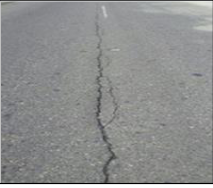
\includegraphics[width=\linewidth]{figs/glon.png}
		\caption*{\centering Grietas longitudinales }
	\end{minipage}
	\hspace{0.5 cm}
	% aquí incluir imagen de  mako
	\begin{minipage}{0.3\linewidth}
		\centering
		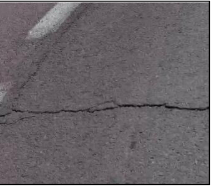
\includegraphics[width=\linewidth]{figs/gtran.png}
		\caption*{\centering Grietas transversales }
	\end{minipage}
	\hspace{0.5 cm}
	\begin{minipage}{0.3\linewidth}
		\centering
		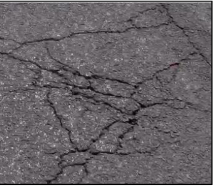
\includegraphics[width=\linewidth]{figs/gpc.png}
		\caption*{\centering Grietas piel de cocodrilo}
	\end{minipage}
	
	\caption{Agrietamiento}
	\label{fig:agrietamiento}
\end{figure}


\begin{figure}[ht!]
	\centering
	\begin{minipage}{0.3\linewidth}
		\centering
		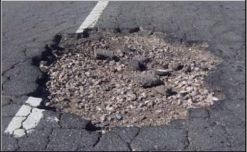
\includegraphics[width=\linewidth]{figs/bache.png}
		\caption*{\centering Bache}
	\end{minipage}
	\hspace{3 cm}
	% aquí incluir imagen de  mako
	\begin{minipage}{0.3\linewidth}
		\centering
		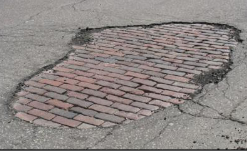
\includegraphics[width=\linewidth]{figs/meteo.png}
		\caption*{\centering Meteorización}
	\end{minipage}
	\hspace{3 cm}
	\begin{minipage}{0.3\linewidth}
		\centering
		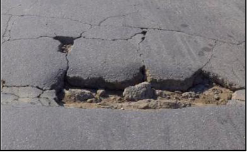
\includegraphics[width=\linewidth]{figs/blandon.png}
		\caption*{\centering Blandón}
	\end{minipage}
	\hspace{3 cm}
	\begin{minipage}{0.3\linewidth}
		\centering
		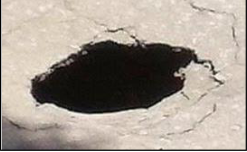
\includegraphics[width=\linewidth]{figs/hueco.png}
		\caption*{\centering Hueco}
	\end{minipage}
	
	\caption{Degradación del material de la capa de rodadura}
	\label{fig:desprendimiento}
\end{figure}


\begin{figure}[ht!]
	\centering
	\begin{minipage}{0.3\linewidth}
		\centering
		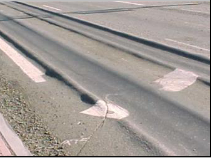
\includegraphics[width=\linewidth]{figs/rod.png}
		\caption*{\centering Roderas }
	\end{minipage}
	\hspace{0.5 cm}
	% aquí incluir imagen de  mako
	\begin{minipage}{0.3\linewidth}
		\centering
		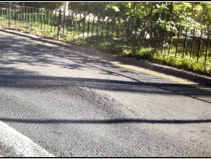
\includegraphics[width=\linewidth]{figs/abo.png}
		\caption*{\centering Abombamiento }
	\end{minipage}
	\hspace{0.5 cm}
	\begin{minipage}{0.3\linewidth}
		\centering
		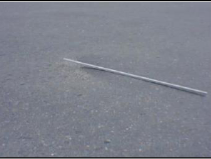
\includegraphics[width=\linewidth]{figs/amp.png}
		\caption*{\centering Ampolla}
	\end{minipage}
	\hspace{0.5 cm}
	\begin{minipage}{0.3\linewidth}
		\centering
		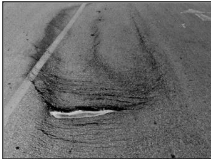
\includegraphics[width=\linewidth]{figs/art.png}
		\caption*{\centering Arrollamiento transversal }
	\end{minipage}
	\hspace{0.5 cm}
	% aquí incluir imagen de  mako
	\begin{minipage}{0.3\linewidth}
		\centering
		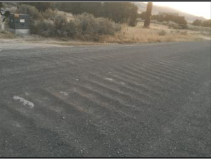
\includegraphics[width=\linewidth]{figs/ond.png}
		\caption*{\centering Ondulaciones }
	\end{minipage}
	\hspace{0.5 cm}
	\begin{minipage}{0.3\linewidth}
		\centering
		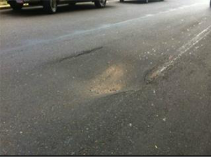
\includegraphics[width=\linewidth]{figs/dep.png}
		\caption*{\centering Depresiones}
	\end{minipage}
	
	
	\caption{Deformación de la capa de rodadura sin degradación de material}
	\label{fig:deformacion}
\end{figure}


\begin{figure}[ht!]
	\centering
	\begin{minipage}{0.3\linewidth}
		\centering
		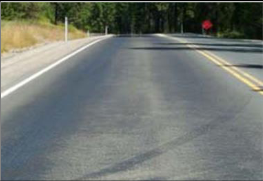
\includegraphics[width=\linewidth]{figs/ex.png}
		\caption*{\centering Exudación }
	\end{minipage}
	\hspace{3 cm}
	% aquí incluir imagen de  mako
	\begin{minipage}{0.3\linewidth}
		\centering
		
\includegraphics[width=\linewidth]{figs/parcheo.png}
		\caption*{\centering Parcheo }
	\end{minipage}
	
	\caption{Otro tipo de daños}
	\label{fig:otro}
\end{figure}

Tras haber mostrado los tipos de deterioros que existen, nos centramos en el mantenimiento de uno de ellos, ya que el problema es muy grande e intentar tratar todos los casos se torna inabarcable para este proyecto. Así, de todos los tipos mostrados, se van a tratar los baches.\\\\\\  % hay 3 saltos de página

Una vez conocido el deterioro en que se va a centrar este proyecto, los organismos existentes en España y todas las oportunidades que un robot \textit{low-cost} ofrece para el mantenimiento de carreteras, se puede decir que este proyecto se centra en el desarrollo de un robot de campo de tamaño compacto y bajo coste, diseñado para ser fácil de usar y controlar. El robot ha sido fabricado completamente mediante impresión 3D y está equipado con herramientas ampliamente utilizadas en el campo de la robótica. Esta combinación permite que cualquier persona, incluso sin un conocimiento profundo en robótica, pueda replicar el robot y ponerlo en funcionamiento. En el próximo capítulo, se presentarán diversos prototipos y futuras aplicaciones que guardan una cierta relación con el tipo de robot desarrollado.

%La conservación de las carreteras es un aspecto fundamental para garantizar la seguridad vial, la eficiencia del transporte y la durabilidad de las infraestructuras viarias. En España, donde la red de carreteras juega un papel crucial en la conectividad y el desarrollo económico, el mantenimiento adecuado de estas infraestructuras es vital para asegurar un tránsito seguro y fluido, así como para prevenir accidentes y reducir los costos derivados del deterioro del pavimento.

%España cuenta con una extensa red de carreteras que incluye autopistas, autovías, carreteras nacionales, autonómicas, y provinciales. Cada una de estas vías requiere un enfoque específico en cuanto a su mantenimiento y conservación, dado que las condiciones de uso y los desafíos asociados varían considerablemente.

%La conservación de las carreteras en el país está regulada y gestionada por diversas instituciones y organismos. La Dirección General de Carreteras\footnote{\url{https://www.transportes.gob.es/carreteras/organizacion-y-funciones/secretaria-general-de-infraestructuras/direccion-general-de-carreteras}}, bajo la gestión del \ac{MITMA}, es la entidad responsable de la Red de Carreteras del Estado, que incluye las vías de mayor envergadura y tráfico. Por su parte, las comunidades autónomas y las diputaciones provinciales gestionan las carreteras que pertenecen a sus respectivas jurisdicciones, como es el caso de las carreteras autonómicas de Castilla-La Mancha\footnote{\url{https://www.castillalamancha.es/gobierno/fomento/estructura/dgfcartra/actuaciones/cat\%C3\%A1logo-y-mapa-de-carreteras-de-castilla-la-mancha}} y las carreteras provinciales de Toledo\footnote{\url{http://eiel.diputoledo.es/visor/index.php}} .

%Además, varias organizaciones juegan un papel destacado en la promoción, estudio y mejora continua de las infraestructuras viarias. El \ac{CEDEX}\footnote{\url{https://www.cedex.es/presentacion}}, por ejemplo, es un organismo de referencia en la investigación y experimentación en el ámbito de las obras públicas y la movilidad. Fundado en 1957, el \acs{CEDEX} trabaja para mejorar y conservar las infraestructuras, impulsar una movilidad segura y sostenible, y proteger el medioambiente.

%Otra entidad relevante es la \ac{AEC}\footnote{\url{https://www.aecarretera.com/quienes-somos}}, una entidad sin ánimo de lucro fundada en 1949, que trabaja en la defensa y promoción de las carreteras. La \acs{AEC} se enfoca en aspectos como la seguridad vial, la sostenibilidad y la calidad de las infraestructuras, adaptando sus actividades a las necesidades y desafíos contemporáneos, como la digitalización y la descarbonización del transporte.


%En el ámbito de la conservación propiamente dicha, la \ac{ACEX}\footnote{\url{https://www.acex.eu/la-asociacion/}}, creada en 1995, agrupa a empresas dedicadas a la conservación de carreteras y se centra en promover la eficiencia y sostenibilidad en el mantenimiento de estas infraestructuras, así como en mejorar la seguridad vial y laboral. También es reseñable destacar sus premios anuales\footnote{\url{https://www.acex.eu/premios-acex/}} que permiten avanzar a pasos agigantados en materia de conservación y seguridad vial.


%Finalmente, cabe destacar la labor de la Plataforma de Trabajadores de Conservación de Carreteras\footnote{\url{https://conservacion.es/index.php?option=com_content&view=article&id=1&Itemid=101}}, un grupo independiente que agrupa a profesionales del sector preocupados por la seguridad laboral, la reducción de la siniestralidad en las actividades de conservación viaria y por mejorar sus condiciones laborales.\\

%Tras conocer a todos los actores que conforman parte del mantenimiento correcto de las carreteras de España, es necesario conocer los tipos de deterioros del pavimento que se tienen que enfrentar.


%\section{Deterioros del pavimento}

%En el artículo \cite{llopis2020deterioros} se presentan los distintos tipos de deterioros o daños en diferentes tipos de pavimentos, así como su rehabilitación y mantenimento. 

%Para entender las distintas categorías de deterioros, es necesario conocer qué es el firme de una carretera y de qué capas está compuesto. El firme es un conjunto de varias capas de materiales seleccionados y, en la mayoría de los casos, tratados, que forman la superestructura de la plataforma. Su propósito es soportar las cargas del tráfico y garantizar que la circulación se realice de manera segura y cómoda. (Figura \ref{fig:firme})

%\begin{figure} [h!]
%	\begin{center}
%		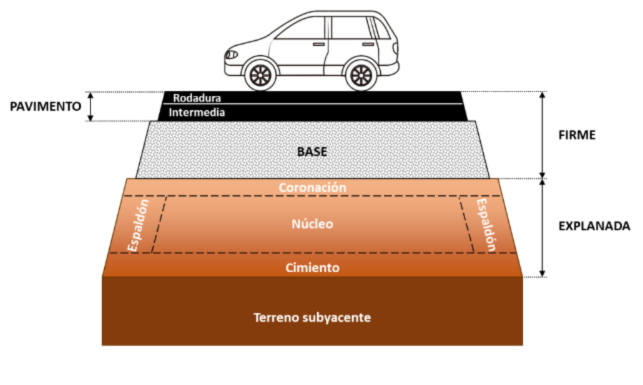
\includegraphics[width=16cm]{figs/firme.png}
%	\end{center}
%	\caption{Firme de una carretera} %\cite{shaw2024leap}}
%\label{fig:firme}
%\end{figure}

%El firme se compone de tres capas: rodadura, capa intermedia y capa base. Las dos primeras forman el pavimento, que soporta las cargas del tráfico y proporciona características como resistencia al deslizamiento y una superficie regular. La capa base, en cambio, tiene una función estructural al absorber las presiones transmitidas y proteger la subbase de cargas excesivas.

%Los firmes se dividen en cuatro tipos: flexibles, semiflexibles, semirrígidos y rígidos. Los firmes flexibles y semiflexibles tienen una capa bituminosa sobre capas granulares. Si el espesor de la capa bituminosa es menor de 15 cm, el firme es flexible; si es mayor, es semiflexible. Los firmes semirrígidos cuentan con un pavimento bituminoso sobre capas tratadas con conglomerantes hidráulicos, con un espesor mínimo de 20 cm. Finalmente, los firmes rígidos tienen un pavimento de hormigón sobre una capa de zahorras.

%\subsubsection{Tipos de deterioros}

%Los distintos tipos de deterioros o daños más comunes que se pueden presentar en
%pavimentos flexibles, semiflexibles y semirrígidos urbanos los podemos clasificar en cuatro grandes categorías: \textit{agrietamiento} (Figura \ref{fig:agrietamiento}), \textit{degradación del material de la capa de rodadura} (Figura \ref{fig:desprendimiento}), \textit{degradación de la capa de rodadura sin degradación de material} (Figura \ref{fig:deformacion}) y \textit{otro tipo de daños} (Figura \ref{fig:otro}). Todo está esquematizado en la Figura \ref{fig:diagrama}.

%%% Incluir aquí las imágenes puestas más arriba 

%Tras haber mostrado toda la gran cantidad de tipos de deterioros que existen, es necesario centrarnos en ser capaces del mantenimiento de uno de ellos ya que el problema es muy grande y sería inabarcable para este proyecto. De todos los tipos mostrados, se van a tratar los \textit{baches}.\\

%\subsubsection{Mantenimiento de baches}

%La reparación de baches en los pavimentos de asfalto es un proceso importante para mantener las carreteras en buen estado. Un bache es una depresión en la superficie de la carretera que puede ser causada por una variedad de factores, como el tráfico pesado, el clima extremo y el envejecimiento del pavimento. Si se dejan sin reparar, los baches pueden causar daños a los vehículos y crear un peligro para los conductores.

%El proceso de reparación de baches comienza con la eliminación del material dañado. Esto se hace mediante el corte del área afectada con una sierra de asfalto o una fresadora. Una vez que se ha eliminado el material dañado, se limpia la superficie hasta dejar el hueco con forma de cuadrilátero regular y se aplica una capa de asfalto fresco. El asfalto se compacta y se alisa para que se ajuste perfectamente al pavimento existente. El resultado final es una superficie de carretera lisa y sin baches\footnote{\url{https://www.youtube.com/watch?v=YPx1bIywgzo}}. En la Figura \ref{fig:repararbache} se puede ver a dos operarios arreglando un bache con asfalto en frío.


%\begin{figure} [h!]
%\begin{center}
%	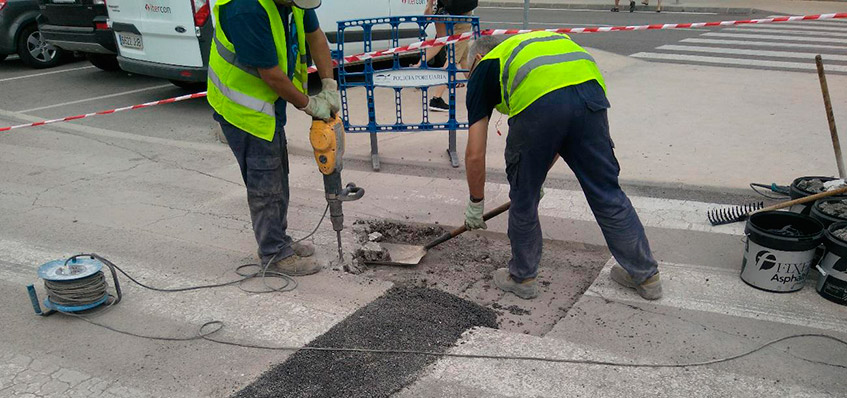
\includegraphics[width=8cm]{figs/repararbache.jpg}
%\end{center}
%\caption{Operarios reparando un bache  $^{\ref{note:reba}}$} %\cite{bidaudrobots}}
%\label{fig:repararbache}
%\end{figure}


%\setcounter{footnote}{30} % Establecer la numeración de la siguiente nota al pie
%\footnotetext[\value{footnote}]{\url{https://fixer.es/blog/como-reparar-bache-con-asfalto-en-frio/}\label{note:reba}}


%Este proyecto se centra en el desarrollo de un robot de campo de tamaño compacto y bajo coste, diseñado para ser fácil de usar y controlar. El robot ha sido fabricado completamente mediante impresión 3D y está equipado con herramientas ampliamente utilizadas en el campo de la robótica. Esta combinación permite que cualquier persona, incluso sin un conocimiento profundo en robótica, pueda replicar el robot y ponerlo en funcionamiento. En el próximo capítulo, se presentarán diversos prototipos y futuras aplicaciones que guardan una cierta relación con el tipo de robot desarrollado.\\


\chapter{Objetivos}
\label{cap:capitulo2}

\begin{flushright}
\begin{minipage}[]{10cm}
\emph{Quizás algún fragmento de libro inspirador...}\\
\end{minipage}\\

Autor, \textit{Título}\\
\end{flushright}

\vspace{1cm}

Escribe aquí un párrafo explicando brevemente lo que vas a contar en este capítulo. En este capítulo lo ideal es explicar cuáles han sido los objetivos que te has fijado conseguir con tu trabajo, qué requisitos ha de respetar el resultado final, y cómo lo has llevado a cabo; esto es, cuál ha sido tu plan de trabajo.\\

\section{Descripción del problema}
\label{sec:descripcion}

Cuenta aquí el objetivo u objetivos generales y, a continuación, concrétalos mediante objetivos específicos.

\section{Requisitos}
\label{sec:requisitos}

Describe los requisitos que ha de cumplir tu trabajo.

\section{Metodología}
\label{sec:metodologia}

Qué paradigma de desarrollo software has seguido para alcanzar tus objetivos.

\section{Plan de trabajo}
\label{sec:plantrabajo}

Qué agenda has seguido. Si has ido manteniendo reuniones semanales, cumplimentando objetivos parciales, si has ido afinando poco a poco un producto final completo, etc.


\chapter{Objetivos}
\label{cap:capitulo3}

\begin{flushright}
\begin{minipage}[]{10cm}
\emph{Establecer metas es el primer paso para convertir lo invisible en visible.}\\
\end{minipage}\\

Tony Robbins\\
\end{flushright}

\vspace{1cm}
\setcounter{footnote}{31} 

Tras haber establecido el marco contextual del presente proyecto, se procede a presentar la descripción del problema, los requisitos, las competencias tanto adquiridas como empleadas, la metodología y el plan de trabajo seguido.

\section{Descripción del problema}
\label{sec:descripcion}

La idea de este trabajo fin de grado nace tras los acontecimientos vividos por la \ac{DANA} que afectó a la zona de Toledo y Madrid el pasado septiembre de 2023. Estos hechos dejaron inundaciones, pueblos anegados, carreteras cortadas, muchos vecinos perdieron sus casas, y desgraciadamente se cobró la vida de tres personas. 

%% Mejorar esta parte por que se da a entender que la dana fue culpa de las carreteras
%Esta situación se produjo, en parte, por la falta de mantenimiento de los pavimentos y carreteras y que posteriormente a lo sucedido, también fue una de las infraestructuras que más tardaron en arreglarse. La principal causa de que eso ocurriese es los bajos recursos y la falta de mano de obra que justamente hay en la zona que sucedieron los hechos. Los operarios que conforman esta mano de obra llevan tiempo exigiendo mejoras de seguridad en su entorno laboral como defiende la Plataforma de Trabajadores de Conservación de Carreteras\footnote{\url{https://conservacion.es/index.php?option=com_content&view=article&id=1&Itemid=101}}.  
Tras lo sucedido, las carreteras fueron las infraestructuras que más tardaron en arreglarse. La principal causa de que eso ocurriese es la falta de fondos, lo que conlleva un escaso mantenimiento. Además, los operarios que conforman la mano de obra llevan tiempo exigiendo mejoras de seguridad en su entorno laboral, como defiende la Plataforma de Trabajadores de Conservación de Carreteras\footnote{\url{https://conservacion.es/index.php?option=com_content&view=article&id=1&Itemid=101}}.
   
La solución propuesta en este trabajo busca ayudar a mejorar esta situación, proporcionando un robot de bajo coste y accesible para cualquier persona y que sirva para poder mejorar el mantenimiento de las carreteras y reducir el riesgo de exposición de los operarios. Por lo tanto, este proyecto pretende, como objetivo principal, crear un robot que, usando materiales de bajo coste, sea capaz de navegar por las carreteras, detectar los baches que vaya encontrando y sea capaz de estimar el área del bache para hacer una estimación media del volumen que ocupa dicho bache y poder ser tapado. De igual manera, todo quedará registrado en una interfaz web en la que cada bache quedará marcado sobre un mapa con su correspondiente descripción para que los operarios puedan operar cuando estimen oportuno.

Con el fin de alcanzar este objetivo principal, se han establecido los siguientes subobjetivos:

\begin{enumerate}
	\item{} Investigar los robots o soluciones actuales que cumplan con las características y objetivos establecidos.
	\item{} Seleccionar los componentes \textit{hardware} de bajo coste necesarios para construir el esqueleto del robot.
	\item{} Analizar las diferentes opciones de diseño que más encajen con la forma del robot.
	\item{} Diseñar las piezas en \acs{CAD} usando herramientas de \textit{software} libre.
	\item{} Usar material típico de impresión 3D para imprimir las partes del robot, como puede ser ABS o PLA. 
	\item{} Desarrollar un modelo del robot para que pueda ser usado en simulación usando herramientas robóticas. 
	\item{} Desarrollar software necesario usando herramientas robóticas para poder controlar el robot físico. 
	\item{} Realizar algunos experimentos en entorno reales o adaptados.  
\end{enumerate}
 

\section{Requisitos}
\label{sec:requisitos}

Tras nombrar los objetivos y subobjetivos a cumplir en este proyecto, se enumeran los requisitos que se han de satisfacer: 

\begin{enumerate}
	\item{} El coste total de la fabricación del robot no debe superar los 250€.
	\item{} Todas las piezas diseñadas deben poderse imprimir en cualquiera impresora convencional.
	\item{} Se usará Ubuntu con soporte a largo plazo como sistema operativo, tanto para el ordenador como para el robot.
	\item{} A fin de facilitar la implementación de este proyecto para cualquier tipo de usuario, no será necesario disponer de ninguna tarjeta gráfica de uso dedicado para entrenar los modelos. 
	\item{} Los modelos entrenados se deben ajustar a las limitaciones hardware del robot.
	\item{} Se busca que sea un proyecto a largo plazo, por eso se debe realizar la integración con la plataforma ROS 2. 
	
	
\end{enumerate}

\section{Competencias}
\label{sec:competencias}

A continuación se detallan las competencias que se han empleado y adquirido para la realización del presente trabajo fin de grado.
   
\subsection{Competencias empleadas}
\label{subsec:competenciase}
Las competencias empleadas para la realización de este proyecto, y que han sido tomadas de las distintas asignaturas del grado, son las siguientes: 

\begin{enumerate}
	\item{Evolución y futuro de la robótica: \textit{CE1.} Capacidad para analizar la evolución de la Ingeniería Robótica y ser capaz de identificar sus aplicaciones, oportunidades de emprendimiento y su impacto en el futuro. 
	Esta competencia ha sido empleada para poder desarrollar los Capítulos 1 y 2 de este proyecto.}
	\item{Laboratorio de sistemas: \textit{CE9.} Capacidad de conocer y manejar los sistemas y las herramientas de las que dispone para su gestión y programación. 
	Esta competencia ha sido empleada para poder configurar y ejecutar código del robot en entornos no gráficos.}
	\item{Sensores y actuadores: \textit{CE12.} Capacidad de diseñar robots y sistemas inteligentes atendiendo a los elementos de sensorización y actuación más adecuados dependiendo de la aplicación, los requerimientos del sistema y las condiciones del entorno. 
	Esta competencia ha sido empleada para poder encontrar los componentes \textit{hardware} necesarios para poder llevar a cabo el esqueleto del robot.}
	\item{Arquitectura \textit{software} para robots: \textit{CE15.} Capacidad de diseñar y programar aplicaciones robóticas y sitemas inteligentes en red usando \textit{middlewares}, mecanismos de comunicación y estándares propios del ámbito de la Ingeniería Robótica. 
	Esta competencia ha sido empleada en el momento de decidir el tipo de arquitectura \textit{software} necesaria a implementar en el robot.}
	\item{Visión artificial: \textit{CE25.} Capacidad de conocer y aplicar métodos de extracción de información a partir de la información percibida por cámaras y sensores 3D al desarrollo de aplicaciones en robots y sistemas inteligentes. 
	Esta competencia ha sido empleada para poder extraer información de la cámara y ser capaz de tratarla.}
	\item{Mecatrónica: \textit{CE32.} Capacidad de diseñar y construir robots móviles. Esta competencia ha sido empleada en el diseño e impresión en 3D de mi robot.}
	\item{Aprendizaje automático: \textit{CE27.} Capacidad de construir sistemas capaces de resolver problemas a partir de información no estructurada proporcionada por ejemplos o por la experiencia. 
	Esta competencia ha sido empleada para poder ser capaz de crear modelos de aprendizaje automático y aplicarlos al robot.}
\end{enumerate}

\subsection{Competencias adquiridas}
\label{subsec:competenciasa}

Las competencias adquiridas con el desarrollo de este trabajo fin de grado, y que aparecen descritas en la guía docente de la propia asignatura, son las siguientes: 

\begin{enumerate}
	\item{\textit{CB2.} Que los estudiantes sepan aplicar sus conocimientos a su trabajo o vocación de una forma profesional y posean las competencias que suelen demostrarse por medio de la elaboración y defensa de argumentos y la resolución de problemas dentro de su área de estudio. 
	Esta competencia se adquiere gracias a la aplicación de las competencias empleadas justificadas anteriormente y que se pueden ver plasmadas en todo el proyecto.}
	\item{\textit{CB4.} Que los estudiantes puedan transmitir información, ideas, problemas y soluciones a un público tanto especializado como no especializado. 
	Esta competencia se aquiere al describir de forma precisa y comprensible todo el proceso complejo implicado en este proyecto dentro del presente documento.}
	\item{\textit{CB5.} Que los estudiantes hayan desarrollado aquellas habilidades de aprendizaje necesarias para emprender estudios posteriores con un alto grado de autonomía. 
	Esta competencia se logra al adquirir el conocimiento suficiente para desarrollar este trabajo de forma totalmente autónoma, contrastando información con distintas fuentes, haciendo pruebas con distintos tipos de \textit{software}, entre otras.}
	\item{\textit{CE28.} Desarrollo de las capacidades adecuadas para realizar un ejercicio original individual (o excepcionalmente colectivo), presentarlo y defenderlo ante un tribunal universitario, consistente en un proyecto en el ámbito de las tecnologías específicas del campo de la Robótica de naturaleza profesional en el que se sinteticen e integren las competencias adquiridas en las enseñanzas.
	Esta última competencia se cumple con el desarrollo de este proyecto: que abarca desde la elección del tema, el conocer el estado del arte, la implementación tanto \textit{hardware} como \textit{software}, el desarrollo de la presente memoria hasta su defensa ante un tribunal.}
\end{enumerate}


\section{Metodología}
\label{sec:metodologia}

Para llevar a cabo este proyecto se ha optado por seguir una metodología que se iniciaba con una profunda investigación sobre el estado del arte para comprobar la viabilidad del desarrollo del presente proyecto. Posteriormente, tras haber elegido el \textit{hardware} necesario para el robot, se decidió usar una metodología experimental que ayudó a decidir el diseño final que tendría el robot. Una vez cumplido esto, se imprimieron y ensamblaron las distintas piezas. 


Para dar soporte \textit{software} al robot real se probó y configuró cada sensor y actuador del robot en distintos sistemas operativos y versiones hasta encontrar la combinación que mejor cumpliese todos los objetivos. Una vez conseguido eso, se decidió seguir un ciclo de desarrollo conocido como \ac{PDCA} y así poder ir haciendo pequeños avances consistentes hasta llegar a una versión completamente funcional. Para el desarrollo del robot simulado también se decidió usar la metodología \acs{PDCA}. Esta metodología sigue los siguientes pasos cíclicos descritos en la imagen \ref{fig:PDCA}. 

%\begin{enumerate}
%	\item{\textit{Planear}}. Ante el problema presentado, se decide qué hacer.
	
%	\item{\textit{Hacer}}. Tras conocer qué hacer, se pone en marcha lo planeado previamente.
	
%	\item{\textit{Comprobar}}. Tras conocer los resultados obtenidos, se comprueban.
	
%	\item{\textit{Actuar}}. Tras comprobar los resultados, se ajusta lo que tiene que ser corregido. 

%\end{enumerate}

\begin{figure} [h!]
	\begin{center}
			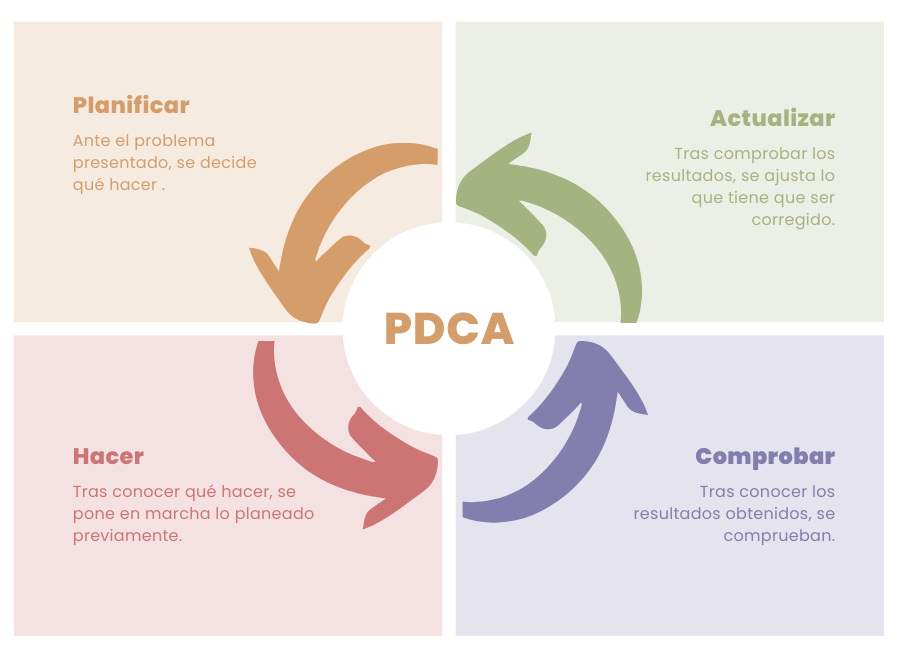
\includegraphics[width=16cm]{figs/PDCA.png}
		\end{center}
	\caption{Método PDCA} 
\label{fig:PDCA}
\end{figure}


\section{Plan de trabajo}
\label{sec:plantrabajo}

El desarrollo del presente trabajo fin de grado se ha dividido en las siguientes etapas: 

\begin{enumerate}
	\item{\textit{Investigación del estado del arte}}. En esta fase inicial, se realizaron búsquedas en plataformas online como Google Scholar\footnote{\url{https://scholar.google.es/}}, Web of Science del FECYT\footnote{\url{https://www.webofscience.com/wos/alldb/basic-search}} que está basa en Web of Science de Clarivate\footnote{\url{https://clarivate.com/products/scientific-and-academic-research/research-discovery-and-workflow-solutions/webofscience-platform/}}, y otras relacionadas con el mantenimiento de carreteras con el fin de encontrar soluciones al problema descrito. 
	
	\item{\textit{Planteamiento hardware del robot}}. Una vez conocida la viabilidad del proyecto, se decidió estudiar qué componentes \textit{low-cost} eran necesarios para dar forma al esqueleto del robot. 
	
	\item{\textit{Diseño de prototipos del robot}}. Tras conocer cuál será el esqueleto del robot, usando cartón y pegamento se hicieron una serie de prototipos hasta encontrar la solución final. Posteriormente se usó la herramienta FreeCAD para modelar las distintas piezas.
	
	\item{\textit{Impresión 3D y emsamblaje de las piezas}}. Una vez el diseño estaba hecho, se decidió imprimirlo usando filamento de tipo PLA azul. Finalmente, se produjo el ensamblaje de todas las piezas.
	
	\item{\textit{Desarrollo del robot en simulación}}. Tras tener el robot completemente montado, se decidió desarrollar el modelo del robot pero esta vez para que se pudiera trabajar con él en simulación; en este caso, usando Gazebo.
	
	\item{\textit{Configuración hardware del robot}}. Tras tener al robot listo en simulación, se decidió configurar cada componente hardware del robot en distintos sistemas operativos hasta encontrar el que mejor encajase con la arquitectura del mismo. 
	
	\item{\textit{Desarrollo software del robot en físico}}. Una vez el robot está completamente configurado y listo para operar en un entorno real, se desarrollaron una serie de nodos en ROS2. Estos ayudan al correcto funcionamiento de cada componente hardware siguiendo el propósito buscado. 
	
	\item{\textit{Experimentos en un entorno real}}. En esta etapa final, se realizaron distintos experimentos en el entorno real para demostrar que se cumplía el objetivo principal.

\end{enumerate}

Asimismo, a lo largo de todo el proceso se ha ido elaborando la presente memoria. La dinámica seguida con el tutor ha sido de reuniones semanales o cada dos semanas, dependiendo de la disponibilidad por las dos partes. En dichas reuniones se comentaban todos los avances realizados y se proponían aspectos a mejorar, sugerencias, y se definían nuevos objetivos a conseguir. 

Todo el contenido del proyecto está alojado en un repositorio público de GitHub\footnote{\url{https://github.com/RoboticsURJC/tfg-jlopez}}. Además, todo el trabajo diario está documentado en el apartado Wiki\footnote{\url{https://github.com/RoboticsURJC/tfg-jlopez/wiki}} de dicho repositorio; dividido en \textit{diario} y en \textit{evolución del proyecto}. El apartado de \textit{diario} trata de contar de forma coloquial qué se ha ido realizando cada día o cada pocos días. Por otro lado, en \textit{evolución del proyecto} se puede encontrar la explicación detallada de ciertos códigos, así como de conceptos teóricos, entre otros detalles.\\\\\\ % 3 saltos de línea

Tras conocer todos los objetivos, subobjetivos, requisitos, competencias, metodología y plan de trabajo llevado a cabo para la realización de este proyecto, se procede a tratar las plataformas de desarrollo usadas. 





\chapter{Plataforma de desarrollo}
\label{cap:capitulo3}

\begin{flushright}
\begin{minipage}[]{10cm}
\emph{Las herramientas adecuadas en las manos adecuadas pueden cambiar el mundo}\\
\end{minipage}\\

Steve Jobs\\
\end{flushright}

\vspace{1cm}

Tras haber establecido los objetivos que se pretenden alcanzar en este proyecto, en este capítulo se van a tratar las distintas plataformas de desarrollo tanto \textit{hardware} como \textit{software} que han contribuido para lograr dichos objetivos.

\section{Hardware}

En este apartado se van a describir el conjunto de componentes hardware que han sido necesarios adquirir para llevar a cabo este proyecto siempre primando por el menor coste de cada componente.

\subsection{Raspberry Pi 4}

La Raspberry Pi es una computadora de bajo coste y con un tamaño compacto que es ideal para proyectos de electrónica, programación y educación. Esta, en su cuarta versión, dispone de un procesador ARM Cortex-A72 de cuatro núcleos a 1,50GHz fabricado en 28nm y con tres configuraciones de memoria. Además, entre otras características, ahora solo necesita una alimentación de USB-C, tiene dos conectores micro HDMI, tiene conexión Wifi, Bluetooh 5.0, dos USB 2.0 y dos USB 3.0. Esta versión de Raspberry permite la compatibilidad con la mayoría de accesorios gracias al conector GPIO de cuarenta pines y el conector \ac{CSI}. Gracias a esos cuarenta pines, el usuario puede interactuar con una amplia variedad de dispositivos externos como sensores, LEDs y motores, lo que lo hace excelente para proyectos de automatización y robótica. 

 Sin embargo, la Raspberry Pi usa procesadores ARM, que, aunque eficientes energéticamente, no están optimizados para realizar tareas intensivas de \ac{IA} como entrenar modelos de redes neuronales o ejecutar inferencias en tiempo real a gran escala. En la figura \ref{fig:raspberry} se puede ver una imagen de la placa con referencia a las distintas partes de la misma. Esta pieza fue prestada por la universidad pero tiene un coste de unos 65€. 


\begin{figure} [h!]
	\begin{center}
		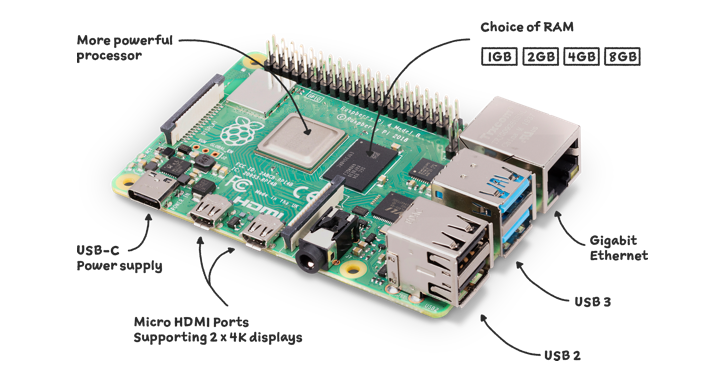
\includegraphics[width=14cm]{figs/raspberrypi4.png}
	\end{center}
	\caption{Raspberry Pi 4$^{\ref{note:enlace35}}$} 
\label{fig:raspberry}
\end{figure}\

\setcounter{footnote}{35} % Establecer la numeración de la siguiente nota al pie
\footnotetext[\value{footnote}]{\url{https://www.raspberrypi.com/products/raspberry-pi-4-model-b/}\label{note:enlace35}}

\subsection{Raspberry Pi cámara}

Esta placa que tiene un tamaño de  23.86 x 25 x 9mm (Figura \ref{fig:raspberrycam}), utiliza el sensor de imagen IMX219PQ de Sony que ofrece imágenes de vídeo de alta velocidad y alta sensibilidad. Dispone también de funciones de control automático como el control de exposición, el balance de blancos y la detección de luminancia. Esta cámara usa un cable plano que se conecta directamente al puerto \ac{CSI}.

Es muy importante destacar su bajo coste, lo que le convierte en muy buena opción para hacer aplicaciones \textit{low-cost}. Sin embargo, el cable de la cámara es bastante sensible a tensiones y torsiones y es debido a ello que aunque la cámara fue prestada por la universidad, fue necesario adquirir una unidad más a través de Amazon con un coste aproximado de 18€.    


\begin{figure} [h!]
	\begin{center}
		\includegraphics[width=6cm]{figs/campi.png}
	\end{center}
	\caption{Raspberry Pi Cámara V2$^{\ref{note:enlace36}}$} 
\label{fig:raspberrycam}
\end{figure}\

\setcounter{footnote}{36} % Establecer la numeración de la siguiente nota al pie
\footnotetext[\value{footnote}]{\url{https://www.raspberrypi.com/products/camera-module-v2/}\label{note:enlace36}}

\subsection{GPS NEO 6M}

Para poder identificar dónde se encuentra cada bache es necesario hacer uso de un posicionamiento global mediante satélites. En este caso se decidió comprar el módulo NEO 6M (Figura \ref{fig:gps}) cuyo asequible precio en Amazon es de 9€. El módulo utiliza el chipset u-blox NEO-6M, que proporciona un seguimiento preciso de la posición utilizando satélites \acs{GPS}, permitiendo determinar la latitud, longitud, altitud, y velocidad. Además, incluye una antena cerámica externa de alta ganancia (puede ser interna en algunas versiones), que mejora la recepción de la señal \acs{GPS}, incluso en áreas con una señal débil.

Tiene una precisión de aproximadamente 2.5 metros en condiciones abiertas. Soporta hasta veintidós satélites simultáneamente, lo que le permite ofrecer posicionamiento confiable y estable. Asimismo, utiliza comunicación por \ac{UART} comunmente a 9600 bps, lo que facilita su integración con muchas placas del mercado.

\begin{figure} [h!]
	\begin{center}
		\includegraphics[width=4cm]{figs/GPSNEO6MV2.jpeg}
	\end{center}
	\caption{Módulo GPS NEO 6M$^{\ref{note:enlace37}}$} 
\label{fig:gps}
\end{figure}\

\setcounter{footnote}{37} % Establecer la numeración de la siguiente nota al pie
\footnotetext[\value{footnote}]{\url{https://www.amazon.es/dp/B088LR3488?ref}\label{note:enlace37}}


\subsection{Sevomotor Estándar Parallax}
Este tipo de servo tiene un rango de rotación de 0 a 180 grados y es compatible su control usando \ac{PWM} con un pulso alto de 0.75–2.25 ms en intervalos de 20 ms (Figura \ref{fig:parallax} izquierda). Estos tipos de servos son muy comunes para utilizar en aplicaciones de animatrónica y robótica. Sin embargo, su coste ha subido en los últimos años y el precio por unidad ronda los 17€. La universidad ha sido quien me ha prestado estos servomotores pero para esta aplicación no es necesario usarlos y se pueden sustituir por otros de menor precio que cumplan con el requisito de tener rotaciones de 0 a 180 grados (Figura \ref{fig:parallax} derecha), cuyo precio de dos servomotores es de casi 8€. 


\begin{figure}[ht!]
	\centering
	\begin{minipage}{0.2\linewidth}
		\centering
		\includegraphics[width=\linewidth]{figs/parallax.png}
		\caption*{\centering Parallax $^{\ref{note:enlace38}}$} %\cite{memnon_image}
	\end{minipage}
	\hspace{2cm}
	% aquí incluir iamgen de Guerrero de terracota
	\begin{minipage}{0.33\linewidth}
		\centering
		\includegraphics[width=\linewidth]{figs/diyi.png}
		\caption*{\centering YIDI $^{\ref{note:enlace39}}$} %\cite{gomezguerreros}
	\end{minipage}
	\caption{Tipos de Servomotores}
	\label{fig:parallax}
\end{figure}


\setcounter{footnote}{38} % Reiniciar la numeración de notas al pie
\footnotetext[\value{footnote}]{\url{https://www.parallax.com/product/parallax-standard-servo/}\label{note:enlace38}}

\setcounter{footnote}{39} % Reiniciar la numeración de notas al pie
\footnotetext[\value{footnote}]{\url{https://es.aliexpress.com/item/1005004551539283.html?spm=a2g0o.productlist.main.15.bee4rd8Srd8SSO&algo_pvid}\label{note:enlace39}}


\subsection{Ruedas ActivityBot}

Para implementar las ruedas de este robot, se decidió tomar las ruedas del kit robótico ActivityBot que usan este tipo de ruedas. Se trata de una rueda de plástico con neumático tipo junta tórica (Figura \ref{fig:wheel}). El perfil estrecho convierte a esta rueda en ideal para aplicaciones que requieren una dirección precisa y el diámetro de la rueda es de 66mm. La universidad ha sido quien me ha prestado su uso pero también se pueden adquirir individualmente con un coste de 4,54€ la unidad.

\begin{figure} [h!]
	\begin{center}
		\includegraphics[width=4cm]{figs/wheel.png}
	\end{center}
	\caption{Rueda ActivityBot$^{\ref{note:enlace40}}$} 
\label{fig:wheel}
\end{figure}\

\setcounter{footnote}{40} % Establecer la numeración de la siguiente nota al pie
\footnotetext[\value{footnote}]{\url{https://es.rs-online.com/web/p/accesorios-para-kits-de-desarrollo/8430897?srsltid=AfmBOorv3a6_tQNdqAoKx_21Mn1m2MAum68oApyvr5mq8ExPTuh_CVNy}\label{note:enlace40}}

\subsection{Google Coral USB}

El Google Coral USB Accelerator (Figura \ref{fig:googlecoral}) es un dispositivo que permite acelerar tareas de \ac{IA} en dispositivos que no cuentan con hardware especializado para ello. Está diseñado para ejecutarse con modelos de aprendizaje automático utilizando la unidad de procesamiento de tensores de Google, lo que mejora significativamente la velocidad de inferencia en aplicaciones de \acs{IA}. Está optimizado para ejecutar modelos preentrenados en TensorFlow Lite, la versión ligera de TensorFlow diseñado para dispositivos con recursos limitados. Sólo es compatible con  las versiones desde Python 3.6 hasta la versión 3.9.

Gracias a todas esas características y para mejorar la detección de baches en tiempo real y solventar las limitaciones de la Raspberry Pi, se ha decidido incluir este componente en el proyecto. Su precio es elevado pero se puede conseguir desde 65€.
 
\begin{figure} [h!]
	\begin{center}
		\includegraphics[width=4cm]{figs/googlecoral.png}
	\end{center}
	\caption{Google Coral USB$^{\ref{note:enlace41}}$} 
	\label{fig:googlecoral}
\end{figure}\

\setcounter{footnote}{41} % Establecer la numeración de la siguiente nota al pie
\footnotetext[\value{footnote}]{\url{https://coral.ai/products/accelerator/}\label{note:enlace41}}

\subsection{Power Bank}

Para poder alimentar a todos los componentes se ha decidido incluir en el proyecto una \textit{power bank} de bastante capacidad para que permita la autonomía del robot durante mucho tiempo. Para ello se ha elegido la Xiaomi Redmi Power Bank de 20000 mAh cuyas dimensiones son: 73,6 x 27,3 x 154 mm. Cuando la adquirí costaba en torno a unos 20€ pero ahora se puede encontrar hasta por el doble de precio. 

\begin{figure} [h!]
	\begin{center}
		\includegraphics[width=5cm]{figs/powerbank.png}
	\end{center}
	\caption{Xiaomi Powerbank$^{\ref{note:enlace42}}$} 
	\label{fig:powerbank}
\end{figure}\

\setcounter{footnote}{42} % Establecer la numeración de la siguiente nota al pie
\footnotetext[\value{footnote}]{\url{https://buy.mi.com/es/item/3202200053}\label{note:enlace42}}

\subsection{Rueda Loca}

Para poder conseguir un movimiento correcto y poder encontrar el punto de apoyo para el robot, es necesario incluir al robot una rueda loca. Tras investigar para encontrar la que mejor encaja, se ha decidido incluir una rueda loca como la que aparece en la Figura \ref{fig:ruedaloca} que tiene las siguientes dimensiones: 5,3 x 2,9 x 2 cm. El precio de una de ellas sale por 1,13€.

\begin{figure} [h!]
	\begin{center}
		\includegraphics[width=4cm]{figs/ruedaloca.png}
	\end{center}
	\caption{Rueda loca$^{\ref{note:enlace43}}$} 
	\label{fig:ruedaloca}
\end{figure}\

\setcounter{footnote}{43} % Establecer la numeración de la siguiente nota al pie
\footnotetext[\value{footnote}]{\url{https://www.amazon.es/dp/B0BZZCJJT8?ref=cm_sw_r_mwn_dp_N64JV6SGENWN4YPSD849&ref_=cm_sw_r_mwn_dp_N64JV6SGENWN4YPSD849&social_share=cm_sw_r_mwn_dp_N64JV6SGENWN4YPSD849&language=es-ES}\label{note:enlace43}}

\subsection{Ordenador principal}

Para poder desarrollar programas, hacer pruebas en simulación, permitir conectarse por SSH a la Raspberry Pi y poder comandar acciones al robot; ha sido necesario tener un ordenador principal que permita realizar todas las tareas. El ordenador que aparece en la Figura \ref{fig:ordenador} es el que se ha empleado en este proyecto y cumple las características descritas en el Cuadro \ref{cuadro:carac_ordena}.


\begin{figure} [h!]
	\begin{center}
		\includegraphics[width=4cm]{figs/ordenador.png}
	\end{center}
	\caption{ASUS VivoBook 14$^{\ref{note:enlace44}}$} 
	\label{fig:ordenador}
\end{figure}\

\setcounter{footnote}{44} % Establecer la numeración de la siguiente nota al pie
\footnotetext[\value{footnote}]{\url{https://www.asus.com/es/laptops/for-home/vivobook/vivobook-14-k413/}\label{note:enlace44}}

\begin{table}[H]
	\begin{center}
		\begin{tabular}{|c|c|}
			\hline
			\textbf{Características} & \textbf{Descripción} \\
			\hline
			Pantalla & 14 pulgadas, Full HD (1920x1080), tecnología LED, antirreflejo \\
			Procesador (CPU) & Intel Core i7 de 10ª generación \\
			Memoria RAM & 8GB \\
			Almacenamiento & 512GB \\
			Tarjeta gráfica (GPU) & Intel UHD Graphics de la serie Comet Lake-U GT2 \\
			Sistema Operativo & Windows 10 y Ubuntu 22.04 \\
			Puertos 1 & 1x USB 3.2 Gen 1 Tipo-A, 1x USB 3.2 Gen 1 Tipo-C, 2x USB 2.0\\  
			Puertos 2 & 1x HDMI, lector de tarjetas microSD, entrada combo de audio \\
			Conectividad & 	Wi-Fi 5 (802.11ac), Bluetooth 4.1 / 5.0 \\
			Batería & 37 Whr \\
			Peso & 1.4 kg \\
			Dimensiones & 32.5 x 21.6 x 1.99 cm \\
			\hline
		\end{tabular}
		\caption{Especificaciones técnicas del ordenador usado}
		\label{cuadro:carac_ordena}
	\end{center}
\end{table}


\section{Software}

En este apartado se van a describir el conjunto de programas y librerías que han sido necesarios usar cumplir con los objetivos del Capítulo 3.

\subsection{FreeCAD}

Esta herramienta de código abierto (Figura \ref{fig:freecad}) es un \textit{software} de diseño asistido por computadora utilizado principalmente para la creación de modelos 3D en diferentes áreas como la ingeniería, arquitectura, y diseño de productos. Está diseñado para ser altamente modular formado por \textit{workbenches}, lo que permite a los usuarios adaptar y extender su funcionalidad según sus necesidades.

FreeCAD se basa en el concepto de modelado paramétrico, lo que permite modificar el diseño fácilmente. Los usuarios pueden retroceder en la historia de un modelo y cambiar parámetros que actualizan automáticamente el diseño. También FreeCAD es multiplataforma, cuenta con una consola de Python integrada y soporta una amplia gama de formatos de archivo como STL y SVG entre otros. Esta ha sido la herramienta elegida para hacer el diseño 3D de la pieza y la generación del formato STL para su posterior impresión. 

\begin{figure} [h!]
	\begin{center}
		\includegraphics[width=3cm]{figs/freecad.png}
	\end{center}
	\caption{Logo de Freecad $^{\ref{note:enlace45}}$} 
	\label{fig:freecad}
\end{figure}\

\setcounter{footnote}{45} % Establecer la numeración de la siguiente nota al pie
\footnotetext[\value{footnote}]{\url{https://www.freecad.org/}\label{note:enlace45}}

\subsection{Python}

Python (Figura \ref{fig:python}) es un lenguaje de programación de alto nivel, interpretado y de propósito general, ampliamente reconocido por su simplicidad y legibilidad. Fue creado por Guido van Rossum y lanzado por primera vez en 1991, y ha crecido rápidamente en popularidad debido a su versatilidad y facilidad de uso tanto para principiantes como para programadores experimentados lo que le convierte en un lenguaje multiplataforma y multiparadigma.

Python es un lenguaje interpretado, lo que significa que el código se ejecuta línea por línea sin necesidad de ser compilado. Esto facilita el desarrollo rápido y la depuración. Tiene una sintaxis sencilla, legible y es ampliamente utilizado en áreas como: desarrollo web (Django y Flask), ciencia de datos y aprendizaje automático (NumPy, Pandas, TensorFlow, y PyTorch), automatización y scripting, entre otros.

Debido a esa simplicidad y versatilidad en Raspberry Pi, se considera Python como uno de los lenguajes de programación oficiales recomendados y es por ello que se ha decidido usar este lenguaje para este proyecto.

\begin{figure} [h!]
	\begin{center}
		\includegraphics[width=4cm]{figs/python.png}
	\end{center}
	\caption{Logo de Python $^{\ref{note:enlace46}}$} 
	\label{fig:python}
\end{figure}\

\setcounter{footnote}{46} % Establecer la numeración de la siguiente nota al pie
\footnotetext[\value{footnote}]{\url{https://es.python.org/}\label{note:enlace46}}

\subsubsection{Software matemático}

NumPy (Numerical Python) es una biblioteca fundamental para el cálculo numérico en Python. Está diseñada para facilitar el manejo eficiente de vectores, grandes matrices y arrays multidimensionales, junto con una amplia colección de funciones matemáticas para realizar operaciones sobre estos arrays. Es tal su poder que se ha dedidido usar en este proyecto para poder calcular el área del bache.

\subsubsection{Software localización}

PyNMEA2 es una biblioteca de Python que se utiliza para analizar y generar mensajes en formato NMEA (National Marine Electronics Association), un estándar utilizado en dispositivos GPS y otros sistemas de navegación marina. Es especialmente útil cuando trabajas con módulos GPS en proyectos de Raspberry Pi u otros dispositivos embebidos, ya que te permite interpretar la información que estos dispositivos envían, como la localización, velocidad y tiempo.

PyNMEA2 te permite interpretar las sentencias NMEA, que son los datos en bruto que los módulos GPS envían, usualmente en forma de texto. Algunas sentencias comunes son:

\$GPGGA: proporciona datos como la latitud, longitud, y altitud.\\
\$GPRMC: contiene información esencial de ubicación, velocidad y tiempo.\\
\$GPGLL: latitud y longitud.

Es este proyecto, se van a emplear las sentencias de \$GPGGA para estimar la ubicación de cada bache.

\subsection{OpenCV}

OpenCV (Figura \ref{fig:opencv}) es una biblioteca de software de código abierto diseñada para la visión artificial y el procesamiento de imágenes. Fue desarrollada inicialmente por Intel en 1999 y ahora es mantenida por una gran comunidad de desarrolladores. OpenCV es ampliamente utilizada en aplicaciones que requieren análisis de imágenes, detección de objetos, reconocimiento de rostros, visión computacional, y mucho más. Gracias a su gran aplicación se ha decidido integrar en el TFG para la detección del bache y el cálculo del área.

\begin{figure} [h!]
	\begin{center}
		\includegraphics[width=3cm]{figs/opencv.png}
	\end{center}
	\caption{Logo de OpenCV $^{\ref{note:enlace47}}$} 
	\label{fig:opencv}
\end{figure}\

\setcounter{footnote}{47} % Establecer la numeración de la siguiente nota al pie
\footnotetext[\value{footnote}]{\url{https://opencv.org/}\label{note:enlace47}}


\subsection{Ubuntu}

Ubuntu (Figura \ref{fig:ubuntu}) es una distribución GNU/Linux basada en Debian GNU/Linux, que incluye principalmente software libre y de código abierto y es mantenida por Canonical Ltd. Puede utilizarse en ordenadores y servidores. Está orientado al usuario promedio, con un fuerte enfoque en la facilidad de uso y en mejorar la experiencia del usuario. Debido a ser software libre es uno de los sistemas operativos más populares y es conocido por su facilidad de uso, estabilidad, amplia comunidad de soporte y por sus actualizaciones periódicas.

\begin{figure} [h!]
	\begin{center}
		\includegraphics[width=4cm]{figs/ubuntu.png}
	\end{center}
	\caption{Logo de Ubuntu $^{\ref{note:enlace48}}$} 
	\label{fig:ubuntu}
\end{figure}\

\setcounter{footnote}{48} % Establecer la numeración de la siguiente nota al pie
\footnotetext[\value{footnote}]{\url{https://ubuntu.com/}\label{note:enlace48}}

Entre todas las versiones existentes para la realización del proyecto se ha usado Ubuntu 22.04 y Ubuntu 20.04. El ordenador usado (descrito en el Apartado 4.1.9) tiene instalado Ubuntu 22.04 \ac{LTS} pero el robot inicialmente usaba Ubuntu 22.04 y finalmente está usando Ubuntu 20.04 \acs{LTS} Server, una versión de Ubuntu sin interfaz gráfica. La decisión de usar Ubuntu 20.04 es debido a que el dispositivo Google Coral USB descrito en el Apartado 4.1.6 es compatible con versiones de Python entre 3.6 y 3.9 siendo en Ubuntu 22.04 la instalación de Python por defecto de 3.10 y el intento de cambiar dicha versión generó numerosos problemas de dependencias sobre todo con la versión de ROS2 usada. En muchos foros tampoco aconsejaban modificar las versiones de Python que vienen instaladas por defecto\footnote{\url{https://github.com/google-coral/pycoral/issues/81}} y que la Rasberry únicamente tuviese esta aplicación se recomienda migrar a Ubuntu 20.04\footnote{\url{https://robotics.stackexchange.com/questions/104413/can-an-ros2-node-run-in-a-venv-and-use-a-different-python-than-that-used-by-the}} que usa Python 3.8. A continuación, se va a mostrar un Cuadro \ref{cuadro:ubuntu} con algunas de las diferencias entre Ubuntu 22.04 y Ubuntu 20.04.

\begin{table}[H]
	\begin{center}
		\begin{tabular}{|c|c|c|}
			\hline
			\textbf{Características} & \textbf{Ubuntu 20.04} & \textbf{Ubuntu 22.04} \\
			\hline
			 Fecha de lanzamiento & Abril 2020 & Abril 2022\\
			 Soporte & Hasta Abril 2025 & Hasta Abril 2027\\
			 Kernel & Linux 5.4 & Linux 5.15 \\
			 Entorno de escritorio & GNOME 3.36 & GNOME 42\\
			 Python & Python 3.8 & Python 3.10\\
			 Soporte gráfico NVIDIA & Soporte estándar & Soporte mejorado con Wayland\\
			\hline
		\end{tabular}
		\caption{Diferencias entre Ubuntu 20.04 y Ubuntu 22.04}
		\label{cuadro:ubuntu}
	\end{center}
\end{table}


\subsection{ROS 2}

Por sus siglas en inglés, \ac{ROS} se trata de un \textit{middleware} para programar robots. Un \textit{middleware} es una capa de software entre el sistema operativo y las aplicaciones de usuario que permiten llevar a cabo aplicaciones \textit{software} independiente del dominio que ese encuentre. Es decir, \acs{ROS} aporta un conjunto de herramientas, bibliotecas y convenciones. También, ofrecen desarrollo, integración, ejecución y herramienta de monitorización. El número 2 indica que es la segunda generación de este middleware. 

\acs{ROS} 2 tiene tres diferentes dimensiones: la comunidad de \acs{ROS} 2 que contribuye al desarrollo de aplicaciones es enorme, el grafo de computación de una aplicación en \acs{ROS} 2 está formado por nodos conectados con distintos paradigmas de comunicación y el espacio de trabajo, también conocido como \textit{workspace}, es aquel que se trata del \textit{software} instalado que se divide a su vez en \textit{underlay} (la instalación básica de \acs{ROS} 2) y \textit{overlay} (son el resto de programas que se desarrollan).

Según se ha explicado en el Apartado 4.2.4, debido a que he necesitado para este proyecto usar Ubuntu 20.04 y Ubuntu 22.04; he tenido que usar las dos distribuciones más estable de \acs{ROS} para cada versión de Ubuntu: \acs{ROS} 2 Foxy y \acs{ROS} 2 Humble respectivamente (Figura \ref{fig:rosdis}).


\begin{figure}[ht!]
	\centering
	\begin{minipage}{0.35\linewidth}
		\centering
		\includegraphics[width=\linewidth]{figs/foxy.png}
		\caption*{\centering Ros2 Foxy $^{\ref{note:enlace51}}$} %\cite{memnon_image}
	\end{minipage}
	\hspace{2cm}
	% aquí incluir iamgen de Guerrero de terracota
	\begin{minipage}{0.35\linewidth}
		\centering
		\includegraphics[width=\linewidth]{figs/humble.png}
		\caption*{\centering Logo Ros2 Humble $^{\ref{note:enlace52}}$} %\cite{gomezguerreros}
	\end{minipage}
	\caption{Distribuciones de \acs{ROS} 2 usadas}
	\label{fig:rosdis}
\end{figure}


% Definir la primera nota al pie con el número 1
\setcounter{footnote}{51} % Reiniciar la numeración de notas al pie
\footnotetext[\value{footnote}]{\url{https://docs.ros.org/en/foxy/Installation.html}\label{note:enlace51}}

\setcounter{footnote}{52} % Reiniciar la numeración de notas al pie
\footnotetext[\value{footnote}]{\url{https://docs.ros.org/en/humble/index.html}\label{note:enlace52}}


\subsubsection{ROS 2 Control}
\acs{ROS} 2 Control\footnote{\url{https://control.ros.org/rolling/doc/getting_started/getting_started.html}} es un framework dentro de \acs{ROS} 2 diseñado para facilitar el control de robots en tiempo real. Proporciona una infraestructura modular y escalable para manejar controladores que gestionan los actuadores (motores, servomotores, etc.) de un robot, así como la lectura de sensores. Se utiliza comúnmente en robots móviles, brazos robóticos, drones y otras plataformas robóticas.

Los componentes principales de \acs{ROS} 2 Control son:

\begin{itemize}
	\item\textit{Controller Manager}. Gestiona controladores e interfaces de hardware en el framework \acs{ROS} 2 Control.
	\item \textit{Resource Manager}. Abstrae y gestiona el hardware, permitiendo la reutilización flexible de componentes.
	\item \textit{Controllers}. Utilizan la teoría de control para interactuar con el hardware.
	\item \textit{User interface}. Pueden interactuar con el sistema mediante servicios y una interfaz de línea de comandos.
	\item \textit{Hardware Components}. Realizan comunicación con hardware físico como puede ser: sistemas, sensores y actuadores.
\end{itemize}\

En este proyecto se ha decidido usar \acs{ROS} 2 Control para crear un modelo del robot en simulación y poder trabajar con él usando la filosofía de \acs{ROS} 2 Control.


\subsection{Gazebo}

Gazebo (Figura \ref{fig:gazebo}) es un simulador de robots que permite modelar entornos físicos tridimensionales y probar robots en ellos sin necesidad de tener el robot en físico y evitar así posibles caídas o golpes. Es ampliamente utilizado en la investigación y desarrollo de robótica, especialmente en combinación con \acs{ROS} y \acs{ROS} 2. Además, ofrece una simulación realista en un entorno 3D y por ello se decidió usar este simulador para el proyecto.

\begin{figure} [h!]
	\begin{center}
		\includegraphics[width=4cm]{figs/gazebo.png}
	\end{center}
	\caption{Logo de Gazebo $^{\ref{note:enlace54}}$} 
	\label{fig:gazebo}
\end{figure}\

\setcounter{footnote}{54} % Establecer la numeración de la siguiente nota al pie
\footnotetext[\value{footnote}]{\url{https://gazebosim.org/home}\label{note:enlace54}}

\subsection{Herramientas de monitorización}

\subsubsection{Rviz}

RViz (Figura \ref{fig:rviz}) es una herramienta de visualización en 3D utilizada en \acs{ROS} y \acs{ROS} 2 para representar información del sistema robótico. Permite a los usuarios ver datos en tiempo real como la posición de un robot, sensores, cámaras, mapas y otros elementos. Se ha utilizado para monitorear el comportamiento del robot en simulación.\\

\begin{figure} [h!]
	\begin{center}
		\includegraphics[width=4cm]{figs/rviz.png}
	\end{center}
	\caption{Logo de Rviz $^{\ref{note:enlace55}}$} 
	\label{fig:rviz}
\end{figure}\

\setcounter{footnote}{55} % Establecer la numeración de la siguiente nota al pie
\footnotetext[\value{footnote}]{\url{http://wiki.ros.org/rviz}\label{note:enlace55}}

\subsubsection{RQT Image View}

RQt Image View \footnote{\url{http://wiki.ros.org/rqt_image_view}} es una herramienta gráfica dentro del ecosistema de \acs{ROS} y \acs{ROS} 2 que permite visualizar imágenes en tiempo real de un flujo de datos de imágenes publicado por una cámara en un sistema robótico. Se ha usado esta herramienta para monitorizar la cámara del robot físico.

\subsubsection{Ros2cli}

\acs{ROS} 2 \ac{CLI}\footnote{\url{https://docs.ros.org/en/humble/Tutorials/Beginner-CLI-Tools.html}} es una herramienta que permite interactuar con el sistema ROS 2 mediante comandos desde la terminal. Ofrece una forma rápida y sencilla de acceder a las funciones y características de \acs{ROS} 2 sin necesidad de escribir o ejecutar código complejo. Ha sido la herramienta principal en este proyecto para ejecutar los distintos nodos, comprobar si estaban bien lanzados, si se producía buena comunicación entre ellos, entre otras aplicaciones.


\subsection{Google Colaboratory}

Google Colaboratory (Figura \ref{fig:googlecolab}) un servicio en la nube proporcionado por Google que permite escribir y ejecutar código en Python a través de un entorno de Jupyter Notebook. No requiere configuración para su uso y proporciona acceso gratuito a recursos de computación, incluidos GPUs y TPUs. Es especialmente usado para el aprendizaje automático, la ciencia de datos y la educación. Gracias a esta herramienta se puede cumplir del apartado 3.2 de Requisitos, el número 4.

\begin{figure} [h!]
	\begin{center}
		\includegraphics[width=4cm]{figs/googlecolab.png}
	\end{center}
	\caption{Logo de Google Colab $^{\ref{note:enlace58}}$} 
	\label{fig:googlecolab}
\end{figure}\

\setcounter{footnote}{58} % Establecer la numeración de la siguiente nota al pie
\footnotetext[\value{footnote}]{\url{https://colab.research.google.com/}\label{note:enlace58}}

\subsection{YOLOv8}

\acs{YOLO}v8 (Figura \ref{fig:yolov8}) desarrollado por la empresa Ultralytics, es una versión avanzada del popular modelo de detección de objetos \ac{YOLO}, diseñado para identificar y localizar objetos en imágenes y videos en tiempo real. Esta versión es conocida por su eficiencia y precisión en la detección de objetos. Es compatible con TensorFlow y PyTorch. También ofrece optimización para diferentes plataformas incluidos como EdgeTPU para dispositivos con recursos limitados como puede ser Raspberry Pi. Debido a todo lo anterior, esta herramienta ha sido elegida para la el entrenamiento del modelo de detección de baches. 

\begin{figure} [h!]
	\begin{center}
		\includegraphics[width=4cm]{figs/yolov8.png}
	\end{center}
	\caption{Logo de YOLOv8 $^{\ref{note:enlace59}}$} 
	\label{fig:yolov8}
\end{figure}\

\setcounter{footnote}{59} % Establecer la numeración de la siguiente nota al pie
\footnotetext[\value{footnote}]{\url{https://docs.ultralytics.com/es}\label{note:enlace59}}


\subsection{TensorFlow Lite}

TensorFlow es una plataforma de código abierto desarrollada por Google para el aprendizaje automático y el desarrollo de redes neuronales. Su diseño permite a los desarrolladores e investigadores crear, entrenar y desplegar modelos de aprendizaje automático de manera eficiente en una variedad de dispositivos, desde ordenadores de alto rendimiento hasta dispositivos con recursos limitados como puede ser Raspberry Pi. Para poder ejecutar modelos en dispositivos una Raspberry se usa TensorFlow Lite (Figura \ref{fig:tflite}) ya que está preparada para optimizar los modelos. Es por ello que cualquier modelo que se quiera usar se tiene que convertir a este formato. 

\begin{figure} [h!]
	\begin{center}
		\includegraphics[width=6cm]{figs/tflite.png}
	\end{center}
	\caption{Logo de TensorFlow Lite $^{\ref{note:enlace60}}$} 
	\label{fig:tflite}
\end{figure}\

\setcounter{footnote}{60} % Establecer la numeración de la siguiente nota al pie
\footnotetext[\value{footnote}]{\url{https://ai.google.dev/edge/litert}\label{note:enlace60}}


\subsection{Interfaz Web}

Para poder hacer más amigable la interacción humano-robot, se ha decidido plasmar los datos obtenidos a través de una interfaz web y para ello se ha decidido usar las siguientes herramientas: 
 
\subsubsection{ROS2bridge Server}

ROS2bridge Server\footnote{\url{http://wiki.ros.org/rosbridge_server}} es parte de ros2bridge\_suite y ofrece una capa de transporte WebSocket para la comunicación bidireccional entre páginas web y \acs{ROS} 2. Convierte mensajes JSON en llamadas a \acs{ROS} 2 y viceversa, permitiendo que las páginas web interactúen con \acs{ROS} 2. 

\subsubsection{OpenStreetMaps}

OpenStreetMaps (Figura \ref{fig:osm}) un proyecto internacional colaborativo desde 2004 que proporciona datos geográficos gratuitos y abiertos, permitiendo la creación de mapas detallados y editables de cualquier parte del mundo por usuarios voluntarios que den crédito a OpenStreetMaps. OpenStreetMaps es utilizado en una amplia gama de aplicaciones, incluyendo navegación, análisis de datos geográficos, y proyectos de código abierto relacionados con mapas y geolocalización.


\begin{figure} [h!]
	\begin{center}
		\includegraphics[width=4cm]{figs/osm.png}
	\end{center}
	\caption{Logo de Open Street Maps $^{\ref{note:enlace62}}$} 
	\label{fig:osm}
\end{figure}\

\setcounter{footnote}{62} % Establecer la numeración de la siguiente nota al pie
\footnotetext[\value{footnote}]{\url{https://www.openstreetmap.org}\label{note:enlace62}}

Tras conocer todas las plataformas de desarrollo para realizar el presente trabajo fin de grado, es el momento de contar el desarrollo completo llevado a cabo para la construcción hardware del robot que se explicará detalladamente en el siguiente capítulo.


\chapter{Diseño y construcción del robot}
\label{cap:capitulo5}

\begin{flushright}
\begin{minipage}[]{10cm}
\emph{La perfección se logra no cuando no hay nada más que añadir, sino cuando no hay nada más que quitar}\\
\end{minipage}\\

Antoine de Saint-Exupéry\\
\end{flushright}

\vspace{1cm}

Tras haber expuesto todas las plataformas de desarrollo utilizadas en este proyecto, en este capítulo se describirá el proceso paso a paso, desde la concepción inicial hasta la construcción y ensamblaje, para que el robot sea completamente operativo.

\section{Geometría del robot}
\label{sec:geometriarobot}

En este apartado se detalla el proceso llevado a cabo para definir la idea y la forma elegida para el robot. La aplicación de este proyecto se encuentra dentro de los robots de campo, y es por ello que estos tipos de robots son mayoritariamente plataformas que trabajan en entornos no estructurados, como se comentó en la Sección \ref{sec:robotcampo}. Por ello, es necesario que la estructura del robot se asemeje a esos tipos de robots y los más comunes son los robots con ruedas. 

Sin embargo, los robots de campo son de gran coste y de grandes dimensiones, lo que hacía inviable que entidades con recursos limitados pudieran adquirirlos. Es por ello que se decidió apostar por los robots de bajo coste. Una primera idea hasta conseguir la solución final al proyecto la tomamos del artículo, \cite{vega18c}, donde los autores nos presentan PiBot (Figura \ref{fig:pibot}), una plataforma robótica educativa de 20 x 10 x 8 cm basada en Raspberry Pi 3 y PiCamera, diseñada para facilitar la enseñanza de robótica a estudiantes de secundaria. Ofrece una infraestructura de \textit{software} abierta en Python y comandos de alto nivel para facilitar el aprendizaje. Además, incluye un modelo 3D imprimible y una versión simulada en Gazebo, disponibles públicamente para que estudiantes y escuelas puedan aprender y practicar robótica sin necesidad del robot físico. 

\begin{figure} [h!]
	\begin{center}
		\includegraphics[width=6cm]{figs/cap5/Original.png}
	\end{center}
	\caption{PiBot} 
	\label{fig:pibot}
\end{figure}

Para poder continuar con la investigación de ese proyecto, se adquirió una unidad del robot PiBot. Además, se creó una estructura de metal para que la cámara cambiase su disposición, mirase hacia el suelo y estuviese orientada de forma natural para evitar futuros cálculos innecesarios. El diseño en este punto quedó como muestra la Figura \ref{fig:pibotmetal}.


\begin{figure} [h!]
	\begin{center}
		\includegraphics[width=8cm]{figs/cap5/new.png}
	\end{center}
	\caption{PiBot con cámara modificada} 
	\label{fig:pibotmetal}
\end{figure}


De PiBot interesa que tiene dos grados de libertad para el movimiento del robot, ya que cuenta con dos ruedas con motores independientes y una rueda loca, lo que le permite desplazarse a lo largo del eje X e Y y, por lo tanto, puede ir hacia delante y atrás y girar sobre sí mismo. Otro grado de libertad que resulta útil en PiBot para su aplicación en este proyecto es el giro sobre el eje Z del motor sobre el que está montada la cámara, lo que le permite aumentar el campo de visión (Figura \ref{fig:esquemaDOF}).


\begin{figure} [h!]
	\begin{center}
		\includegraphics[width=9cm]{figs/cap5/dof.jpg}
	\end{center}
	\caption{Esquema de los grados de libertad de PiBot} 
	\label{fig:esquemaDOF}
\end{figure}


Una vez puesto en marcha el PiBot, se realizaron una serie de modificaciones \textit{hardware} para poder cumplir con el objetivo principal descrito en la Sección \ref{sec:descripcion}; fue necesario añadir una serie de componentes \textit{hardware} a PiBot para poder formar el esqueleto completo del nuevo prototipo robótico, que fue bautizado como PiBotJ. A continuación se describen detalladamente los distintos componentes \textit{hardware}.

\section{Disposición de los componentes hardware}
\label{sec:disposicionhardware}

Una vez conocido las características que eran útiles de PiBot para PiBotJ, se definió la disposición de los componentes \textit{hardware}, descritos en la Sección \ref{sec:hardware}, para poder confeccionar el esqueleto completo. La Figura \ref{fig:fritzzing} muestra todas la conexiones que fueron necesarias usar en la Raspberry Pi para dar soporte a todos los componentes del PiBotJ. 

\begin{figure} [h!]
	\begin{center}
		\includegraphics[width=10cm]{figs/cap5/modelocompleto_bb3.png}
	\end{center}
	\caption{Esquema de conexiones del PiBotJ} 
	\label{fig:fritzzing}
\end{figure}


La alimentación a la placa se realiza a través del puerto USB-C. En uno de los puertos USB 3.0 se conectó el Google Coral y, en el puerto CSI, la Raspberry PiCamera. Asimismo, sobre los pines se conectaron los servomotores estándar de Parallax y el módulo GPS. Para el servomotor derecho fue necesario usar el pin 4 para el cable de alimentación, el pin 12 (GPIO 18) para el cable de la señal y el pin 6 para el cable de tierra. Para el servomotor izquierdo fue necesario usar el pin 2 para el cable de alimentación, el pin 7 (GPIO 4) para el cable de la señal y el pin 9 para el cable de tierra. Finalmente, para el módulo GPS había que conectarlo al puerto serie y fue necesario usar el pin 1 para el cable de la alimentación, el pin 10 (GPIO 15) para el cable de transmisión de señal (TX), el pin 8 (GPIO 14) para el cable de recepción de señal (RX) y el pin 14 para el cable de tierra. 

 
\section{Bocetos}
\label{sec:bocetos}

La realización de bocetos es una etapa fundamental en el proceso de diseño, que se realiza antes de iniciar el modelado en 3D, ya que su propósito es obtener una visión clara de la estructura y disposición de los componentes que conforman el PiBotJ. Una vez que se definió el esqueleto completo que este necesitaba, se creó una serie de bocetos (Figura \ref{fig:bocetos}) que permitieron afinar los detalles antes de realizar el diseño en 3D.

\begin{figure}[ht!]
	\centering
	\begin{minipage}{0.4\linewidth}
		\centering
		\includegraphics[width=\linewidth]{figs/cap5/prototipo_laser.jpeg}
	\end{minipage}
	\hspace{2cm}
	\begin{minipage}{0.4\linewidth}
		\centering
		\includegraphics[width=\linewidth]{figs/cap5/prototipo_sin_laser.jpeg}
	\end{minipage}
	\hspace{2cm}
	\begin{minipage}{0.5\linewidth}
		\centering
		\includegraphics[width=\linewidth]{figs/cap5/boceto_papel.jpeg}
	\end{minipage}
	\caption{Bocetos creados a mano}
	\label{fig:bocetos}
\end{figure}

Antes de realizar el diseño \acs{CAD} de las piezas se creó una maqueta a tamaño real (Figura \ref{fig:maqueta2}) para poder tener una idea de cómo sería la aplicación final y así intentar no malgastar material de impresión. Tras tener una idea clara de cómo iba a ser PiBotJ, se comenzó con el diseño de cada una de las piezas.  

%\begin{figure}[ht!]
%	\centering
%	\begin{minipage}{0.5\linewidth}
%		\centering
%		\includegraphics[width=\linewidth]{figs/cap5/boceto_carton1.jpeg}
%		\caption*{\centering}
%	\end{minipage}
%	\hspace{1cm}
%	\begin{minipage}{0.4\linewidth}
%		\centering
%		\includegraphics[width=\linewidth]{figs/cap5/boceto_carton2.jpeg}
%		\caption*{\centering}
%	\end{minipage}
%	\hspace{2cm}
%	\begin{minipage}{0.4\linewidth}
%		\centering
%		\includegraphics[width=\linewidth]{figs/cap5/boceto_carton3.jpeg}
%		\caption*{\centering}
%	\end{minipage}
%	\caption{Maqueta en proceso}
%	\label{fig:maqueta1}
%\end{figure}

\begin{figure}[ht!]
	\centering
	%\begin{minipage}{0.44\linewidth}
	%	\centering
	%	\includegraphics[width=\linewidth]{figs/cap5/boceto_carton4.jpeg}
	%	\caption*{\centering}
	%\end{minipage}
	%\hspace{2cm}
	\begin{minipage}{0.4\linewidth}
		\centering
		\includegraphics[width=\linewidth]{figs/cap5/boceto_carton5.jpeg}
		\caption*{\centering}
	\end{minipage}
	\hspace{2cm}
	%\begin{minipage}{0.45\linewidth}
	%	\centering
	%	\includegraphics[width=\linewidth]{figs/cap5/boceto_carton6.jpeg}
	%	\caption*{\centering}
	%\end{minipage}
	%\hspace{2cm}
	\begin{minipage}{0.4\linewidth}
		\centering
		\includegraphics[width=\linewidth]{figs/cap5/boceto_carton7.jpeg}
		\caption*{\centering}
	\end{minipage}
	\caption{Maqueta creada}
	\label{fig:maqueta2}
\end{figure}


\section{Diseño CAD}
\label{sec:diseñocad}

Para hacer el diseño \acs{CAD} y la maqueta explicada en el apartado anterior, se crearon unos planos a mano (Figura \ref{fig:planos}) de las diferentes piezas involucradas en el diseño. Las medidas fueron precisas gracias al uso del calibre.


\begin{figure}[ht!]
	\centering
	\begin{minipage}{0.45\linewidth}
		\centering
		\includegraphics[width=\linewidth]{figs/cap5/planos1.jpeg}
		\caption*{\centering}
	\end{minipage}
	\hspace{1cm}
	\begin{minipage}{0.45\linewidth}
		\centering
		\includegraphics[width=\linewidth]{figs/cap5/planos2.jpeg}
		\caption*{\centering}
	\end{minipage}
	\hspace{1cm}
	\begin{minipage}{0.45\linewidth}
		\centering
		\includegraphics[width=\linewidth]{figs/cap5/planos3.jpeg}
		\caption*{\centering}
	\end{minipage}
	\hspace{1cm}
	\begin{minipage}{0.45\linewidth}
		\centering
		\includegraphics[width=\linewidth]{figs/cap5/planos4.jpeg}
		\caption*{\centering}
	\end{minipage}
	\caption{Planos de los componentes}
	\label{fig:planos}
\end{figure}


%\begin{figure}[ht!]
%	\centering
%	\begin{minipage}{0.4\linewidth}
%		\centering
%		\includegraphics[width=\linewidth]{figs/cap5/calib1.jpeg}
%		\caption*{\centering}
%	\end{minipage}
%	\hspace{2cm}
%	\begin{minipage}{0.4\linewidth}
%		\centering
%		\includegraphics[width=\linewidth]{figs/cap5/calib2.jpeg}
%		\caption*{\centering}
%	\end{minipage}
%	\caption{Comprobación mediante calibre}
%	\label{fig:calibre}
%\end{figure}

\setcounter{footnote}{64}

Para el diseño de PiBotJ se empleó la herramienta de modelado FreeCAD\footnote{\url{https://www.freecad.org/}}, con el objetivo de utilizar \textit{software} libre, permitiendo que cualquier persona pueda acceder y modificar las piezas. El diseño se dividió en cuatro partes, cada una de las cuáles tenía una finalidad específica, descritas a continuación.

Para llevar a cabo el diseño de todas las piezas se han seguido los tutoriales de dos cursos de FreeCAD: el del profesor Juan González (también conocido como \textit{Obijuan})\footnote{\url{https://www.youtube.com/watch?v=2_DbFzFV9D4}}, y el de dcahue-ingeniería\footnote{\url{https://www.youtube.com/watch?v=4zp2DrWv8Wk}}, ambos fundamentales en el desarrollo del proyecto. Además, se han utilizado otros tutoriales específicos, como los dedicados a la creación de \textit{shape binders}\footnote{\url{https://www.youtube.com/watch?v=MCY5IrWrHrU}} y la realización de planos inclinados\footnote{\url{https://www.youtube.com/watch?v=T4hKW1mLrCw}}, esenciales para diseñar la inclinación de la cámara.

\subsection{Chasis}
\label{subsec:chasis}

La estructura principal, que da soporte al robot, fue diseñada para alojar los motores de las ruedas y de la cámara. En la parte trasera se incorporó un prisma rectangular, destinado a la colocación de la rueda loca, mientras que en el lado izquierdo se le dotó con un orificio circular para sujetar la \textit{power bank}. En la parte superior se añadieron seis aberturas rectangulares, para permitir el paso ordenado de los cables, manteniendo una estética limpia y organizada desde el exterior.

Además, a este chasis se le dotó de cuatro orificios circulares, que permitieron fijar la carcasa mediante tornillos. Se puede encontrar tanto su versión compatible con FreeCAD\footnote{\url{https://github.com/RoboticsURJC/tfg-jlopez/blob/main/design/base.FCStd}}, como con el formato de diseño 3D por excelencia, STL\footnote{\url{https://github.com/RoboticsURJC/tfg-jlopez/blob/main/design/base.stl}}. La Figura \ref{fig:pbase} (izquierda) muestra el chasis, tal como será preparada para la impresión en una impresora 3D convencional. Por su parte, la Figura \ref{fig:pbase} (derecha) presenta nuevamente el chasis, pero esta vez equipada con los componentes de \textit{hardware} necesarios.

\begin{figure}[ht!]
	\centering
	\begin{minipage}{0.45\linewidth}
		\centering
		\includegraphics[width=\linewidth]{figs/cap5/basevistasuperiorsin.png}
		\caption*{\centering} % Vista superior
	\end{minipage}
	\hspace{1cm}
	\begin{minipage}{0.45\linewidth}
		\centering
		\includegraphics[width=\linewidth]{figs/cap5/basecon2.png}
		\caption*{\centering}
	\end{minipage}
	\caption{Distintas vistas del chasis}
	\label{fig:pbase}
\end{figure}

%\begin{figure}[ht!]
%	\centering
%	\begin{minipage}{0.45\linewidth}
%		\centering
%		\includegraphics[width=\linewidth]{figs/cap5/basevistasuperiorsin.png}
%		\caption*{\centering} % Vista superior
%	\end{minipage}
%	\hspace{1cm}
%	\begin{minipage}{0.45\linewidth}
%		\centering
%		\includegraphics[width=\linewidth]{figs/cap5/basevistaladosin.png}
%		\caption*{\centering} % Vista inferior
%	\end{minipage}
	%\hspace{1cm}
	%\begin{minipage}{0.45\linewidth}
	%	\centering
	%	\includegraphics[width=\linewidth]{figs/cap5/basevistalateralsin.png}
	%	\caption*{\centering} % Vista lateral
	%\end{minipage}
	%\hspace{1cm}
	%\begin{minipage}{0.45\linewidth}
	%	\centering
	%	\includegraphics[width=\linewidth]{figs/cap5/basetraserasin.png}
	%	\caption*{\centering} % Vista lateral izquierdo
	%\end{minipage}
	
%	\caption{Distintas vistas del chasis}
%	\label{fig:pbase}
%\end{figure}


%\begin{figure}[ht!]
%	\centering
%	\begin{minipage}{0.45\linewidth}
%		\centering
%		\includegraphics[width=\linewidth]{figs/cap5/basecon1.png}
%		\caption*{\centering}
%	\end{minipage}
%	\hspace{1cm}
%	\begin{minipage}{0.45\linewidth}
%		\centering
%		\includegraphics[width=\linewidth]{figs/cap5/basecon2.png}
%		\caption*{\centering}
%	\end{minipage}
%	\caption{Distintas vistas del chasis atornillado}
%	\label{fig:pbasemontada}
%\end{figure}

\subsection{Soporte de la cámara}
\label{subsec:soportecamara}

Para posicionar la cámara de manera que mire hacia el suelo y pueda captar los baches, fue necesario fijarla con una rotación sobre el eje y. En este caso, dicha rotación fue de 50 grados, o 130 grados si se toma como referencia la base de la pieza que va atornillada al motor (Figura \ref{fig:rot}). Esta base fue dotada con dos orificios diagonales que permiten su fijación al motor.

\begin{figure} [h!]
	\begin{center}
		\includegraphics[width=8cm]{figs/cap5/rot.png}
	\end{center}
	\caption{Inclinación de la cámara} 
\label{fig:rot}
\end{figure}

A la parte inclinada de la pieza se le incluyó un orificio diseñado para alojar el sensor CMOS, garantizando una correcta alineación y visión. Además, esta sección fue dotada con dos orificios adicionales para asegurar el sensor CMOS y mantenerlo firmemente en su lugar. Se puede encontrar tanto su versión compatible con FreeCAD\footnote{\url{https://github.com/RoboticsURJC/tfg-jlopez/blob/main/design/camara.FCStd}} como con el formato STL\footnote{\url{https://github.com/RoboticsURJC/tfg-jlopez/blob/main/design/camara.stl}}. La Figura \ref{fig:pcamara} (izquierda) muestra el soporte de la cámara, tal como será preparada para la impresión en una impresora 3D convencional. Por su parte, la Figura \ref{fig:pcamara} (derecha) presenta nuevamente el soporte de la cámara, pero esta vez atornillado sobre los componentes \textit{hardware} necesarios. 

\begin{figure}[ht!]
	\centering
	\begin{minipage}{0.45\linewidth}
		\centering
		\includegraphics[width=\linewidth]{figs/cap5/camera3sin.png}
		\caption*{\centering}
	\end{minipage}
	\hspace{1cm}
	\begin{minipage}{0.45\linewidth}
		\centering
		\includegraphics[width=\linewidth]{figs/cap5/camera2con.png}
		\caption*{\centering}
	\end{minipage}
	\caption{Distintas vistas del soporte de la cámara}
	\label{fig:pcamara}
\end{figure}

%\begin{figure}[ht!]
%	\centering
	%\begin{minipage}{0.45\linewidth}
	%	\centering
	%	\includegraphics[width=\linewidth]{figs/cap5/camera2sin.png}
	%	\caption*{\centering}
	%\end{minipage}
	%\hspace{1cm}
%	\begin{minipage}{0.45\linewidth}
%		\centering
%		\includegraphics[width=\linewidth]{figs/cap5/camera3sin.png}
%		\caption*{\centering}
%	\end{minipage}
%	\hspace{1cm}
	
	%\caption{Distintas vistas del soporte de la cámara}
	%\label{fig:pcamara}
	%\end{figure}
	
	%\begin{figure}[ht!]
	%\centering
%	\begin{minipage}{0.45\linewidth}
%		\centering
%		\includegraphics[width=\linewidth]{figs/cap5/camera2con.png}
%		\caption*{\centering}
%	\end{minipage}
	%\hspace{1cm}
	%\begin{minipage}{0.45\linewidth}
	%	\centering
	%	\includegraphics[width=\linewidth]{figs/cap5/camera3con.png}
	%	\caption*{\centering}
	%\end{minipage}
%	\caption{Distintas vistas del soporte de la cámara}
%	\label{fig:pcamara}
%\end{figure}


\subsection{Carcasa}
\label{subsec:carcasa}

Esta carcasa fue diseñada para alojar la placa Raspberry Pi, el módulo GPS y la \textit{power bank} en su interior. La cara superior fue dotada de doce orificios circulares, destinados a atornillar tanto la Raspberry Pi como el módulo GPS, y seis aberturas que se conectaban con la cara inferior, alineándose con las aberturas correspondientes del chasis, para garantizar un paso de cables ordenado.

La cara inferior, además de las seis aberturas, fue dotada con cuatro orificios adicionales para permitir el atornillado del chasis. En el lateral izquierdo, la pieza se dejó abierta para facilitar la inserción de la \textit{power bank}, mientras que en el lado derecho se añadieron dos cuadrantes que permitieron retirar la \textit{power bank} cuando sea necesario. Esta pieza está disponible tanto en formato compatible con FreeCAD\footnote{\url{https://github.com/RoboticsURJC/tfg-jlopez/blob/main/design/parte-superior.FCStd}} como en STL\footnote{\url{https://github.com/RoboticsURJC/tfg-jlopez/blob/main/design/parte-superior.stl}}.

La Figura \ref{fig:psuperior} (izquierda) muestra la carcasa, lista para la impresión en una impresora 3D convencional. La Figura \ref{fig:psuperior} (derecha) presenta nuevamente la carcasa, pero equipada con los componentes \textit{hardware} necesarios.


%\begin{figure}[ht!]
%	\centering
%	\begin{minipage}{0.45\linewidth}
%		\centering
%		\includegraphics[width=\linewidth]{figs/cap5/superior1.png}
%		\caption*{\centering} % vista superior 
%	\end{minipage}
%	\hspace{1cm}
%	\begin{minipage}{0.45\linewidth}
%		\centering
%		\includegraphics[width=\linewidth]{figs/cap5/superior2.png}
%		\caption*{\centering} % vista inferior
%	\end{minipage}
%	\hspace{1cm}
%	\begin{minipage}{0.45\linewidth}
%		\centering
%		\includegraphics[width=\linewidth]{figs/cap5/superior3.png}
%		\caption*{\centering}  % vista lateral 
%	\end{minipage}
%	\hspace{1cm}
%	\begin{minipage}{0.45\linewidth}
%		\centering
%		\includegraphics[width=\linewidth]{figs/cap5/superior4.png}
%		\caption*{\centering} % vista lateral izquierdo
%	\end{minipage}
	
%	\caption{Distintas vistas de la carcasa}
%	\label{fig:psuperior}
%\end{figure}


%\begin{figure}[ht!]
%	\centering
%	\begin{minipage}{0.45\linewidth}
%		\centering
%		\includegraphics[width=\linewidth]{figs/cap5/superior1m.png}
%		\caption*{\centering}
%	\end{minipage}
%	\hspace{1cm}
%	\begin{minipage}{0.45\linewidth}
%		\centering
%		\includegraphics[width=\linewidth]{figs/cap5/superior2m.png}
%		\caption*{\centering}
%	\end{minipage}
%	\caption{Distintas vistas de la carcasa atornillada}
%	\label{fig:psuperiormontada}
%\end{figure}

\begin{figure}[ht!]
	\centering
	\begin{minipage}{0.45\linewidth}
		\centering
		\includegraphics[width=\linewidth]{figs/cap5/superior2.png}
		\caption*{\centering} % vista inferior
	\end{minipage}
	\hspace{1cm}
	\begin{minipage}{0.45\linewidth}
		\centering
		\includegraphics[width=\linewidth]{figs/cap5/superior1m.png}
		\caption*{\centering}
	\end{minipage}
	\caption{Distintas vistas de la carcasa}
	\label{fig:psuperior}
\end{figure}


\subsection{Sujección trasera}
\label{subsec:sujecciontrasera}

Para asegurar que la \textit{power bank} se mantenga en su lugar dentro del robot, se diseñó una pieza que se atornilla en el lado izquierdo del chasis. Esta pieza fue definida como un prisma rectangular con más de 30 mm de altura, aproximadamente 5 mm de largo y 3 mm de ancho (Figura \ref{fig:ptrasera} izquierda). La pieza debe colocarse en posición vertical para evitar que la \textit{power bank} se deslice, y en posición horizontal cuando se desea extraer esta. Existe una versión en FreeCAD\footnote{\url{https://github.com/RoboticsURJC/tfg-jlopez/blob/main/design/sujeccion-trasera.FCStd}} y otra en formato STL\footnote{\url{https://github.com/RoboticsURJC/tfg-jlopez/blob/main/design/sujeccion-trasera.stl}}. La Figura \ref{fig:ptrasera} (derecha) muesta cómo quedaría montada la pieza sobre el robot.

%\begin{figure}[ht!]
%	\centering
%	\begin{minipage}{0.45\linewidth}
%		\centering
%		\includegraphics[width=\linewidth]{figs/cap5/trasera1.png}
%		\caption*{\centering}
%	\end{minipage}
%	\hspace{1cm}
%	\begin{minipage}{0.45\linewidth}
%		\centering
%		\includegraphics[width=\linewidth]{figs/cap5/trasera2.png}
%		\caption*{\centering}
%	\end{minipage}
%	\caption{Distintas vistas de la pieza para la sujección trasera}
%	\label{fig:ptrasera}
%\end{figure}

%\begin{figure} [h!]
%	\begin{center}
%		\includegraphics[width=8cm]{figs/cap5/traseracon.png}
%	\end{center}
%	\caption{Pieza para la sujección trasera atornillada} 
%	\label{fig:traseracon}
%\end{figure}

\begin{figure}[ht!]
	\centering
	\begin{minipage}{0.45\linewidth}
		\centering
		\includegraphics[width=\linewidth]{figs/cap5/trasera2.png}
		\caption*{\centering}
	\end{minipage}
	\hspace{1cm}
	\begin{minipage}{0.45\linewidth}
		\centering
		\includegraphics[width=\linewidth]{figs/cap5/traseracon.png}
		\caption*{\centering}
	\end{minipage}
	\caption{Distintas vistas de la pieza para la sujección trasera}
	\label{fig:ptrasera}
\end{figure}

Una vez detalladas cada una de las piezas \acs{CAD} diseñadas, se continúa describiendo el proceso de impresión y montaje que se ha seguido para conseguir finalmente el prototipo robótico PiBotJ.
  
\section{Impresión y montaje}
\label{sec:impresionmontaje}

En esta sección se presentan todos los detalles que deben considerarse para replicar este proyecto mediante impresión 3D. 

En nuestro caso, para la impresión de PiBotJ, se usó la impresora FDM Creality Ender3 V2 (Figura \ref{fig:impresora}), un rollo de PLA convencional azul y Ultimaker Cura\footnote{\url{https://ultimaker.com/es/software/ultimaker-cura/}} como \textit{software} de impresión. Para la impresión de todas las piezas se emplearon las mismas características que muestra el Cuadro \ref{cuadro:cimpresion}. Para este proyecto fue necesario imprimir una pieza de cada una de las explicadas en el apartado de Diseño CAD (Sección \ref{sec:diseñocad}), como muestra la Figura \ref{fig:piezasimpresas}. La duración de impresión fue en torno a 50 horas.
 
\begin{figure} [h!]
	\begin{center}
		\includegraphics[width=7cm]{figs/cap5/impresora.jpg}
	\end{center}
	\caption{Impresora FDM Creality Ender3 V2$^{\ref{note:enlace79}}$} 
	\label{fig:impresora}
\end{figure}

\setcounter{footnote}{79} % Establecer la numeración de la siguiente nota al pie
\footnotetext[\value{footnote}]{\url{https://www.creality.com/es/products/ender-3-v2-neo-3d-printer}\label{note:enlace79}}

\begin{table}[H]
	\begin{center}
		\begin{tabular}{|c|c|}
			\hline
			Características & Parámetros\\
			\hline
			\multirow{2}{*}{Calidad} & \multirow{2}{*}{\shortstack{ Altura de capa: 0,2 mm \\ Ancho de línea: 0,4 mm}}\\
			& \\
			\hline
			\multirow{4}{*}{Paredes} & \multirow{4}{*}{\shortstack{Grosor de pared: 0,8 mm \\ Cantidad de líneas de pared: 2 \\ Alineación de costura en Z: \textit{Esquina más afilada} \\ Preferencia de costura en esquina: \textit{Ocultación inteligente} }} \\
			& \\
			& \\
			& \\
			\hline
			
			\multirow{2}{*}{\shortstack{Relleno}} &  \multirow{2}{*}{\shortstack{Densidad de relleno: 15\% \\ Patrón de relleno: \textit{Gyroid} }}\\
			& \\
			\hline
			\multirow{2}{*}{\shortstack{Velocidad}} &  \multirow{2}{*}{\shortstack{Velocidad de impresión: 50 mm/s\\ Velocidad de la primera capa: 20 mm/s}}\\
			& \\
			\hline
		\end{tabular}
		\caption{Características usadas para la impresión}
		\label{cuadro:cimpresion}
	\end{center}
\end{table}


\begin{figure} [h!]
	\begin{center}
		\includegraphics[width=10cm]{figs/cap5/setcompleto.jpeg}
	\end{center}
	\caption{Piezas impresas} 
	\label{fig:piezasimpresas}
\end{figure}


Una vez impresas todas las piezas y retirados sus soportes generados, fue el momento del montaje, cuya duración fue de dos horas aproximadamente, pero puede ser más dependiendo de las habilidades del usuario.

Uno de los elementos que se tuvo que tener en cuenta para el montaje fueron los Hama Beads. Los Hama Beads son cilindros de plástico pequeños con un círculo en el centro usados comunmente para manualidades y para la creación de objetos de decoración. En este caso, se usaron para evitar que tanto la Raspberry Pi como el módulo GPS toquen directamente la superficie impresa. Además, por su círculo interior pasaban perfectamente los tornillos usados. 

%Uno de los elementos que se tuvo que tener en cuenta para el montaje fueron los Hama Beads (Figura \ref{fig:hamabeads}). Los Hama Beads son cilindros de plástico pequeños con un círculo en el centro usados comunmente para manualidades y para la creación de objetos de decoración. En este caso, se usaron para evitar que tanto la Raspberry Pi como el módulo GPS toquen directamente la superficie impresa. Además, por su círculo interior pasaban perfectamente los tornillos usados. 

%\begin{figure} [h!]
%	\begin{center}
%		\includegraphics[width=6cm]{figs/cap5/hama.png}
%	\end{center}
%	\caption{Hama Beads$^{\ref{note:enlace80}}$} 
%	\label{fig:hamabeads}
%\end{figure}

\setcounter{footnote}{80} % Establecer la numeración de la siguiente nota al pie
\footnotetext[\value{footnote}]{\url{https://www.hamabeads.es/}\label{note:enlace80}}


Otro aspecto a tener en cuenta es que, para la placa del módulo GPS, fue necesario soldarle unos pines (Figura \ref{fig:soldar}) para posteriormente conectarle los cables sin pérdidas de señal. También fue necesario agrandar con una taladradora los cuatro agujeros que tiene la antena del módulo para que puedan entrar bien los tornillos. 

\begin{figure} [h!]
	\begin{center}
		\includegraphics[width=8cm]{figs/cap5/soldar.jpeg}
	\end{center}
	\caption{Soldando pines al módulo GPS} 
	\label{fig:soldar}
\end{figure}

Una vez solventados los contratiempo anteriores, se puede pasar a la fase de fijación de piezas mediante tornillos. El Cuadro \ref{cuadro:tornillos} muestra toda la tornillería necesaria.Los tornillos, tuercas y arandelas se pueden obtener en cualquier ferretería. Se recomienda usar un fijador para evitar que se aflojen los tornillos.

Además, las Figuras \ref{fig:pbasemontada}, \ref{fig:pcamaramontada}, \ref{fig:psuperiormontada} y \ref{fig:traseracon} han sido tomadas gracias a un diseño creado en FreeCAD\footnote{\url{https://github.com/RoboticsURJC/tfg-jlopez/blob/main/design/robotcompleto.FCStd}}, de PiBotJ completo, que muestra el lugar donde se sitúa la tornillería del robot y ayudará al usuario facilitar el ensamblaje. La Figura \ref{fig:robotfreecad} muestra el robot completo montado. Para conseguir realizar el diseño de PiBotJ completo en FreeCAD, se tomaron los ficheros .stl obtenidos de la Sección \ref{sec:diseñocad}. Además, se tuvo que diseñar aparte: la antena del módulo \acs{GPS}, la batería, la rueda loca, un Hama Bead y la rueda; todos los ficheros se pueden encontrar en la carpeta \verb|misc|\footnote{\url{https://github.com/RoboticsURJC/tfg-jlopez/tree/main/design/misc}}. La placa del módulo \acs{GPS} necesitó ser editada partiendo de una versión de Thinkercad\footnote{\url{https://www.tinkercad.com/things/6etb23HSw0w-gy-neo6mv2-neo-6m}} y, por otro lado, el resto de componentes se tomaron de la librería de FreeCAD\footnote{\url{https://github.com/FreeCAD/FreeCAD-library/tree/master}}.

\begin{table}[H]
	\begin{center}
		\begin{tabular}{|c|c|c|c|c|}
			\hline
			Componente & Tornillos & Tuercas & Arandelas & Hama Beads blancas\\
			\hline
			Motores & 12 M2 10mm & 12 & 24 &\\
			\hline
			Picamera (base) & 2 M2 10mm & 2 & 4 &\\
			\hline
			Picamera (cámara) & 2 M2 12mm & 2 & 12 &\\
			\hline
			Raspberry Pi & 4 M2 12mm & 4 & & 4\\
			\hline
			Placa GPS & 4 M2 16mm & 4 & 8 & 4\\
			\hline
			Antena GPS & 4 M2 16mm & 4 & & 4\\
			\hline
			Sujección entre placas & 4 M2 16mm & 4 & 8 &\\
			\hline
			Sujección trasera & 1 M2 16mm & 1 & 2 &\\
			\hline
		\end{tabular}
		\caption{Tornillería necesaria}
		\label{cuadro:tornillos}
	\end{center}
\end{table}

\begin{figure} [h!]
	\begin{center}
		\includegraphics[width=12cm]{figs/cap5/completo3.png}
	\end{center}
	\caption{Robot completo montado en FreeCAD} 
	\label{fig:robotfreecad}
\end{figure}


Para sujetar el cable de alimentación de la Raspberry Pi se utilizó una brida. Para optimizar el espacio ocupado por los cables se emplearon gomas pequeñas. Además, fue necesario utilizar diez cables macho-hembra para alimentar los dos motores y el módulo GPS, mientras que el motor de la cámara se quedó sin conectar, ya que la cámara se va a mantener fija, dejando su movilidad como una posible línea futura de trabajo.

Respecto a las ruedas, se han probado dos tipos: las del kit \textit{ActivityBot} y las de goma azul genéricas. Según la aplicación, se puede optar por una u otra. A continuación, se explicará el montaje de cada tipo.

Para utilizar las ruedas del kit \textit{ActivityBot} simplemente fue necesario atornillarlas al robot con el tornillo que viene incluido, ya que estas ruedas fueron diseñadas específicamente para motores Parallax. El aspecto del robot con este tipo de ruedas es el que muestra la Figura \ref{fig:ab}.

\begin{figure} [h!]
	\begin{center}
		\includegraphics[width=12cm]{figs/cap5/ab.jpeg}
	\end{center}
	\caption{PiBotJ con ruedas de ActivityBot} 
	\label{fig:ab}
\end{figure}

Por otro lado, para poder usar la ruedas genéricas, fue necesario realizar algunas modificaciones. En primer lugar, se usó una sierra para cortar las partes sobrantes (Figura \ref{fig:rae}, izquierda). También fue necesario perforar la rueda con un taladro para que el tornillo que conecta al motor encajara fácilmente. Y, tras esto, fue necesario colocar dos topes de motor sobre la superficie lisa de la rueda (Figura \ref{fig:rae}, derecha) y hacer los agujeros correspondientes para atornillarlos. En este caso, se utilizaron siete tornillos M2 de 8 mm. El aspecto del robot con este tipo de ruedas es el que muestra la Figura \ref{fig:ra}.

\begin{figure}[ht!]
	\centering
	\begin{minipage}{0.45\linewidth}
		\centering
		\includegraphics[width=\linewidth]{figs/cap5/creacionra1.jpeg}
		\caption*{\centering}
	\end{minipage}
	\hspace{1cm}
	\begin{minipage}{0.45\linewidth}
		\centering
		\includegraphics[width=\linewidth]{figs/cap5/creacionra2.jpeg}
		\caption*{\centering}
	\end{minipage}
	\caption{Ensamblaje ruedas azules genéricas}
	\label{fig:rae}
\end{figure}


\begin{figure} [h!]
	\begin{center}
		\includegraphics[width=12cm]{figs/cap5/ra.jpeg}
	\end{center}
	\caption{PiBotJ con ruedas azules} 
	\label{fig:ra}
\end{figure}

En el Capítulo de Experimentos se verá qué rueda funciona mejor según el tipo de superficie. Para resumir lo explicado, el Cuadro \ref{cuadro:costetotal} enumera todos los componentes necesarios para construir a PiBotJ, junto con sus respectivos precios.

\begin{table}[H]
	\begin{center}
		\begin{tabular}{|c|c|}
			\hline
			Componente & Precio \\
			\hline
			Motores Parallax & 34€ \\
			\hline
			Picamera &  18€ \\
			\hline
			Raspberry Pi & 65€ \\
			\hline
			Módulo GPS & 9€ \\
			\hline
			Ruedas ActivityBot/Azules & 9€ \\
			\hline
			Google Coral USB & 65€ \\
			\hline
			Powerbank & 20€ \\
			\hline
			Rueda Loca & 1,13€ \\
			\hline
			Tornillos, tuercas, arandelas y Hama Beads & 3€ \\
			\hline
			Cables, gomas y brida & 3€ \\
			\hline
			Rollo de PLA gastado & 10€ \\
			\hline
		\end{tabular}
		\caption{Coste proyecto}
		\label{cuadro:costetotal}
	\end{center}
\end{table}

El coste total del proyecto es de 237,13€, por lo que está por debajo del límite establecido de 250€, cumpliendo de este modo con el objetivo establecido en la Sección \ref{sec:descripcion}.\\\\\\\\\\



Llegados a este punto, se ha completado el diseño y contrucción del prototipo robótico PiBotJ. A continuación, se detallará el soporte \textit{software} que se ha dado a este robot para alcanzar el objetivo del proyecto.



\chapter{Soporte software del robot}
\label{cap:capitulo6}

\begin{flushright}
\begin{minipage}[]{10cm}
\emph{El software es una gran combinación entre arte e ingeniería}\\
\end{minipage}\\

Bill Gates\\
\end{flushright}

\vspace{1cm}
\setcounter{footnote}{82}

Una vez contado todo el proceso llevado a cabo para el diseño y construcción del prototipo robótico, en este capítulo se aborda el soporte software en el robot para ponerlo en funcionamiento tanto en simulación como en la vida real.

\section{Simulación}

En esta sección se va a tratar el proceso seguido para conseguir poner a PiBotJ en funcionamiento a través de simulación, en concreto usando Gazebo. Esta parte ha sido desarrollada en el ordenador principal que se ha usado para este proyecto, explicado en el Capítulo 4, y por tanto, usa Ubuntu 22.04 LTS y ROS 2 Humble. Para conseguir la simulación, ha sido necesario tener instalado ROS 2 Humble\footnote{\url{https://docs.ros.org/en/humble/Installation.html}} y seguir los siguientes pasos de instalación: 

\begin{verbatim}
	sudo apt update && sudo apt upgrade
	sudo apt install ros-humble-ros2-control ros-humble-ros2-controllers
	sudo apt install ros-humble-rviz2
	sudo apt install ros-humble-gazebo-ros-pkgs
	sudo apt install ros-humble-xacro ros-humble-robot-state-publisher 
	sudo apt install ros-humble-joint-state-publisher
\end{verbatim}

Una vez instalado todos los programas, fue el momento de empezar a desarrollar el código. 

\subsection{URDF/Xacro}

Primero de todo fue necesario definir las estructuras y propiedades del robot. Para ello, se decidió usar el formato \ac{URDF}\footnote{\url{http://wiki.ros.org/urdf}} y \textit{Xacro}\footnote{\url{http://wiki.ros.org/xacro}}, muy comunes en aplicaciones robóticas. \acs{URDF} usa un formato de ficheros XML y describe al robot como un conjunto de \textit{links} (enlaces), que están conectadas por una serie de \textit{joints} (uniones). Mientras que \textit{Xacro} usa también un formato de ficheros XML que permite crear URDF de manera más modular, reutilizable y eficiente mediante el uso de macros y propiedades. Para más información se puede consultar la siguiente fuente\footnote{\url{https://articulatedrobotics.xyz/tutorials/ready-for-ros/urdf/}}.

En este proyecto se decidió crear una serie de ficheros \textit{Xacro}, cada uno dedicado a las distintas partes del robot (\verb|camera.xacro|\footnote{\url{https://github.com/RoboticsURJC/tfg-jlopez/blob/main/code/ros2/src/pibotj_r2c/description/camera.xacro}}, \verb|gps.xacro|\footnote{\url{https://github.com/RoboticsURJC/tfg-jlopez/blob/main/code/ros2/src/pibotj_r2c/description/gps.xacro}} y \verb|robot_core.xacro|\footnote{\url{https://github.com/RoboticsURJC/tfg-jlopez/blob/main/code/ros2/src/pibotj_r2c/description/robot_core.xacro}}). Cada fichero \textit{Xacro} sigue siempre la mismas etiquetas de \verb|<joint>| y \verb|<link>|, empleadas según convenga. Es importante tener en cuenta herramientas como validadores de XML\footnote{\url{https://www.xmlvalidation.com/index.php?id=1&L=0\#xml-9-6--1732781305}} para evitar problemas.

Existen cuatro tipos de \textit{joint}: \textit{prismatic}, \textit{continuous}, \textit{revolute} y \textit{fixed}. En el Código \ref{cod:fj} se puede ver la definición de una \textit{fixed joint}; si se quiere usar otro tipo de \textit{joint}, hay que añadir algunos campos\footnote{\url{https://articulatedrobotics.xyz/tutorials/ready-for-ros/urdf/\#joint-tags}}.

\begin{code}[h]
	\begin{lstlisting}[language=xml]
		<joint name="gps_joint" type="fixed">
			<parent link="chassis"/>
			<child link="gps_frame"/>
			<origin xyz="-0.1 0.0 0.04" rpy="0 0 0"/>
		</joint>
	\end{lstlisting}
	\caption[Macro que define \textit{fixed joint}]{Macro que define una \textit{fixed joint}}
	\label{cod:fj}
			\end{code}

En relación a los \textit{link}, obligatoriamente tienen que tener las macros de \verb|<visual>|, \verb|<collision>| e \verb|<inertial>|, sino pueden surgir errores\footnote{\url{https://answers.gazebosim.org//question/25166/problem-changing-joint-from-fixed-to-revolute/}}. Existen cuatro tipos de geometría: \textit{box}, \textit{cylinder}, \textit{sphere} y \textit{mesh}. El Código \ref{cod:ml} muestra un ejemplo de una \textit{mesh link} pero si se quiere tratar más ejemplos, se puede consultar la siguiente fuente\footnote{\url{https://articulatedrobotics.xyz/tutorials/ready-for-ros/urdf/\#link-tags}}.

\begin{code}[h]
	\begin{lstlisting}[language=xml]
		<link name="camera_link">
			<visual>
				<origin xyz="0.02 0.01 0.0 " rpy="0 0 ${-pi/2}"/>
				<geometry>
					<mesh filename="package://pibotj_r2c/meshes/camara.stl" scale="0.001 0.001 0.001"/>
				</geometry>
				<material name="Blue">
					<color rgba="${0/255} ${0/255} ${255/255} 1.0"/>
				</material>
			</visual>
			<collision> 
				<origin xyz="0.0 0.0 0.0 " rpy="0 0 ${-pi/2}"/>
				<geometry>
					<mesh filename="package://pibotj_r2c/meshes/camara.stl" scale="0.001 0.001 0.001"/>
				</geometry>
			</collision>
			<inertial>
				<origin xyz="0.0 0.0 0.0" rpy="0 0 ${-pi/2}"/>
				<mass value="0.03"/> <!--30g-->
				<inertia ixx="0.01" ixy="0.0" ixz="0.0" iyy="0.005" iyz="0.0" izz="0.005"/>
			</inertial>
		</link>
	\end{lstlisting}
	\caption[Macro que define una \textit{mesh link}]{Macro que define una \textit{mesh link}}
	\label{cod:ml}
\end{code}


Una vez definidas las distintas partes del robot, fue el momento de incluir en los distintos ficheros las interacciones del robot con el simulador y para ello se usa la macro \verb|<gazebo>|.En el presente proyecto, se ha simulado el sensor cámara y el módulo \ac{GPS}. Existen muchos tipos de interacciones pero el Código \ref{cod:gazebo} muestra cómo simular el sensor cámara. Para simular el módulo GPS se ha utilizado un mensaje del tipo NavSatFix\footnote{\url{http://docs.ros.org/en/api/sensor_msgs/html/msg/NavSatFix.html}}. Si se quiere tratar más ejemplos, se puede consultar la siguiente fuente\footnote{\url{http://wiki.ros.org/urdf/XML/Gazebo}}.

\begin{code}[h]
	\begin{lstlisting}[language=xml]
		<gazebo reference="camera_link_optical">
		<material>Gazebo/Blue</material>
			<sensor name="camera" type="camera">
				<pose> 0 0 0 0 0 0 </pose>
				<visualize>true</visualize>
				<update_rate>10</update_rate>
				<camera>
					<horizontal_fov>1.089</horizontal_fov>
					<image>
						<format>R8G8B8</format>
						<width>640</width>
						<height>480</height>
					</image>
					<clip>
						<near>0.05</near>
						<far>8.0</far>
					</clip>
				</camera>
				<plugin name="camera_controller" filename="libgazebo_ros_camera.so">
					<frame_name>camera_link_optical</frame_name>
				</plugin>
			</sensor>
		</gazebo>
	\end{lstlisting}
	\caption[Macro que permite a Gazebo simular una cámara]{Macro que permite a Gazebo simular una cámara}
	\label{cod:gazebo}
\end{code}

En el presente proyecto se han definido los sistemas de coordenadas que aparecen en la Figura \ref{fig:links}. Una vez se definió el robot y los sensores necesarios para que Gazebo interactuara con el modelo, era el momento de usar ROS 2 Control. 

\begin{figure} [h!]
	\begin{center}
		\includegraphics[width=12cm]{figs/cap6/links.png}
	\end{center}
	\caption{Sistemas de Coordenadas de PiBotJ}
	\label{fig:links}
\end{figure}\


\subsection{ROS 2 Control}

\subsubsection{Hardware Components/Interfaces}

 Tienen una comunicación directa con el hardware y existen tres tipos; en este caso, se decidió declarar todo el robot como un sistema para no limitar así el número de sensores y actuadores. 
 
 Si se quiere comprobar los hardware interfaces que tiene cualquier sistema, se puede hacer usando el siguiente comando: 
 \verb|ros2 control list_hardware_interfaces|

 
 Se puede ver que hay: (mostrar foto de output)
 
 %command interfaces
 %camera_joint/position [available] [claimed]
 %left_wheel_joint/velocity [available] [claimed]
 %right_wheel_joint/velocity [available] [claimed]
 %state interfaces
 %camera_joint/position
 %left_wheel_joint/position
 %left_wheel_joint/velocity
 %right_wheel_joint/position
 %right_wheel_joint/velocity
 
 Cada una de las command interfaces y state interfaces han sido definidas  para que el resource manager lo pueda usar gracias a la etiqueta <ros2\_control>. Dentro de esas etiquetas se asigna a cada joint el tipo de controller que se quiere usar. 
 
 Cada Hardware interface se configura usando un URDF. 
 
 
\subsubsection{Controllers}


Existen muchos tipos de controllers ya definidos, pero para este proyecto vamos a usar 2 tipos: diferencial y por posición. Para ello, es necesario definir sus parámetros a través de .yaml. 
En este caso, se llama my\_controllers.yaml. 



La rotación de la cámara (imagen y explicar cómo va)
ros2 Control  explicarlo


Creación de los topics que se quiera, la cámara por posición 

los topics que hay que lanzar 

he tenido que incluir el topic de la cámara, gps y de los motores

una vez se lanza el robot por primera vez puede fallar o tardar mucho, volver a lanzarlo


Explicar los topics que aparecen una vez ejecutado. 

Mostrar el video con el resultado final (rehacerlo)


\subsection{Robot State Publisher }

\subsection{Launcher}



\subsection{Ejemplo en funcionamiento}








\section{Vida real}

Configuración y comprobar que todas las partes funcionan

Explicar software creado para las dos versiones: teleoperado y autónomo

Modelo pin hole...

Shoelace method...

Capítulo 6: incluir lo de openvision paper\\









\section{Snippets}

Puede resultar interesante, para clarificar la descripción, mostrar fragmentos de código (o \textit{snippets}) ilustrativos. En el Código \ref{cod:codejemplo} vemos un ejemplo escrito en \texttt{C++}.

\begin{code}[h]
	\begin{lstlisting}[language=C++]
		void Memory::hypothesizeParallelograms () {
			for(it1 = this->controller->segmentMemory.begin(); it1++) {
				squareFound = false; it2 = it1; it2++;
				while ((it2 != this->controller->segmentMemory.end()) && (!squareFound)) {
					if (geometry::haveACommonVertex((*it1),(*it2),&square)) {
						dist1 = geometry::distanceBetweenPoints3D ((*it1).start, (*it1).end);
						dist2 = geometry::distanceBetweenPoints3D ((*it2).start, (*it2).end);
					}
					// [...]
				\end{lstlisting}
				\caption[Función para buscar elementos 3D en la imagen]{Función para buscar elementos 3D en la imagen}
				\label{cod:codejemplo}
			\end{code}
			
			En el Código \ref{cod:codejemplo2} vemos un ejemplo escrito en \texttt{Python}.
			
			\begin{code}[h]
				\begin{lstlisting}[language=Python]
					def mostrarValores():
					print (w1.get(), w2.get())
					
					master = Tk()
					w1 = Scale(master, from_=0, to=42)
					w1.pack()
					w2 = Scale(master, from_=0, to=200, orient=HORIZONTAL)
					w2.pack()
					Button(master, text='Show', command=mostrarValores).pack()
					
					mainloop()
				\end{lstlisting}
				\caption[Cómo usar un Slider]{Cómo usar un Slider}
				\label{cod:codejemplo2}
			\end{code}
			
			\section{Verbatim}
			
			Para mencionar identificadores usados en el código ---como nombres de funciones o variables--- en el texto, usa el entorno literal o verbatim \verb|hypothesizeParallelograms()|. También se puede usar este entorno para varias líneas, como se ve a continuación:
			
			\begin{verbatim}
				void Memory::hypothesizeParallelograms () {
					// add your code here
				}
			\end{verbatim}
			
			\section{Ecuaciones}
			
			Si necesitas insertar alguna ecuación, puedes hacerlo. Al igual que las figuras, no te olvides de referenciarlas. A continuación se exponen algunas ecuaciones de ejemplo: Ecuación \ref{ec:ec1} y Ecuación \ref{ec:ec2}.
			
			\begin{myequation}[h]
				\begin{equation}
					H = 1 - \frac{\sum_{i=0}^{N}\frac{(\frac{d_{j_s} + d_{j_e}}{2})}{N}}{M}
					\nonumber
					\label{ec:ec1}
				\end{equation}
				\caption[Ejemplo de ecuación con fracciones]{Ejemplo de ecuación con fracciones}
			\end{myequation} 
			
			\begin{myequation}[h]
				\begin{equation}
					v(entrada)= \left\{
					\begin{array}{lcc}
						0 & \mbox{if} & \epsilon_t < 0.1\\
						K_p\cdot{(T_{t}-T)} & \mbox{if}& 0.1 \leq \epsilon_t < M_t\\
						K_p \cdot M_t & \mbox{if}& M_t < \epsilon_t
					\end{array}
					\right.
					\label{ec:ec2}
				\end{equation}
				\caption[Ejemplo de ecuación con array y letras y símbolos especiales]{Ejemplo de ecuación con array y letras y símbolos especiales}
			\end{myequation}
			
			\section{Tablas o cuadros}
			
			Si necesitas insertar una tabla, hazlo dígnamente usando las propias tablas de \LaTeX, no usando pantallazos e insertándolas como figuras... En el Cuadro \ref{cuadro:ejemplo} vemos un ejemplo.
			
			\begin{table}[H]
				\begin{center}
					\begin{tabular}{|c|c|}
						\hline
						\textbf{Parámetros} & \textbf{Valores} \\
						\hline
						Tipo de sensor & Sony IMX219PQ[7] CMOS 8-Mpx \\
						Tamaño del sensor & 3.674 x 2.760 mm (1/4" format) \\
						Número de pixels & 3280 x 2464 (active pixels) \\
						Tamaño de pixel & 1.12 x 1.12 um \\
						Lente & f=3.04 mm, f/2.0 \\
						Ángulo de visión & 62.2 x 48.8 degrees \\
						Lente SLR equivalente & 29 mm \\
						\hline
					\end{tabular}
					\caption{Parámetros intrínsecos de la cámara}
					\label{cuadro:ejemplo}
				\end{center}
			\end{table}
			
			En los textos puedes poner palabras en \textit{cursiva}, para aquellas expresiones en sentido \textit{figurado}, palabras como \textit{robota}, que está fuera del diccionario castellano, o bien para resaltar palabras de una colección: \textit{(a)} es la primera letra del abecedario, \textit{(b)} es la segunda, etc.\\
			
			Al poner las dos líneas del anterior párrafo, este aparecerá separado del anterior. Si no las pongo, los párrafos aparecerán pegados. Sigue el criterio que consideres más oportuno.
			
			\section{Segunda sección}
			\label{sec:segundaseccion}
			
			No olvides incluir imágenes y referenciarlas, como la Figura \ref{fig:roomba}.
			
			\begin{figure} [h!]
				\begin{center}
					\includegraphics[width=8cm]{figs/roomba}
				\end{center}
				\caption{Robot aspirador Roomba de iRobot.}
				\label{fig:roomba}
			\end{figure}\
			
			Ni tampoco olvides de poner las URLs como notas al pie. Por ejemplo, si hablo de la Robocup\footnote{\url{http://www.robocup.org}}.
			
			\subsection{Números}
			\label{sec:subseccion}
			
			En lugar de tener secciones interminables, como la Sección \ref{sec:robotica}, divídelas en subsecciones.
			
			Para hablar de números, mételos en el entorno \textit{math} de \LaTeX, por ejemplo, $1.5Kg$. También puedes usar el símbolo del Euro como aquí: 1.500\euro.
			
			\subsection{Listas}
			
			Cuando describas una colección, usa \texttt{itemize} para ítems o \texttt{enumerate} para enumerados. Por ejemplo:
			
			\begin{itemize}
				\item \textit{Entorno de simulación.} Hemos usado dos entornos de simulación: uno en 3D y otro en 2D.
				\item \textit{Entornos reales.} Dentro del campus, hemos realizado experimentos en Biblioteca y en el edificio de Gestión.
			\end{itemize}\
			
			\begin{enumerate}
				\item Primer elemento de la colección.
				\item Segundo elemento de la colección.
			\end{enumerate}\
			
			\paragraph{Referencias bibliográficas}
			\label{sec:referencias}
			
			Cita, sobre todo en este capítulo, referencias bibliográficas que respalden tu argumento. Para citarlas basta con poner la instrucción \verb|\cite| con el identificador de la cita. Por ejemplo: libros como \cite{vega12e}, artículos como \cite{vega19b}, URLs como \cite{vega19a}, tesis como \cite{vega18b}, congresos como \cite{vega18a}, u otros trabajos fin de grado como \cite{vega08b}.
			
			Las referencias, con todo su contenido, están recogidas en el fichero \texttt{bibliografia.bib}. El contenido de estas referencias está en formato \texttt{BibTex}. Este formato se puede obtener en muchas ocasiones directamente, desde plataformas como \texttt{Google Scholar} u otros repositorios de recursos científicos.
			
			Existen numerosos estilos para reflejar una referencia bibliográfica. El estilo establecido por defecto en este documento es APA, que es uno de los estilos más comunes, pero lo puedes modificar en el archivo \texttt{memoria.tex}; concretamente, cambiando el campo \verb|apalike| a otro en la instrucción \verb|\bibliographystyle{apalike}|. 
			
			\
			
			\
			
			\
			
			Y, para terminar este capítulo, resume brevemente qué vas a contar en los siguientes.


\section{Corrector ortográfico}

Una vez tengas todo, no olvides pasar el corrector ortográfico de \LaTeX a todos tus ficheros \textit{.tex}. En \texttt{Windows}, el propio editor \texttt{TeXworks} incluye el corrector. En \texttt{Linux}, usa \texttt{aspell} ejecutando el siguiente comando en tu terminal:

\begin{verbatim}
aspell --lang=es --mode=tex check capitulo1.tex
\end{verbatim}


\chapter{Experimentos}
\label{cap:capitulo7}

\begin{flushright}
\begin{minipage}[]{10cm}
\emph{Toda la vida es un experimento. Cuantos más experimentos hagas, mejor.}\\
\end{minipage}\\

Ralph Waldo Emerson\\
\end{flushright}

\vspace{1cm}

\setcounter{footnote}{117} % Establecer la numeración de la siguiente nota al pie

En este capítulo se tratarán los diferentes experimentos llevados a cabo para la realización de este proyecto y que han permitido conseguir y demostrar la consecución del objetivo y subobjetivos definidos en la Sección \ref{sec:descripcion}.

\section{Impresión 3D}
\label{sec:expimpresion3d}
Aparte de la solución proporcionada en la Sección \ref{sec:impresionmontaje}, se probaron previamente distintas opciones de diseño y de impresión 3D hasta encontrar la mejor opción.

Primero, se optó por diseñar la estructura como una pieza única para facilitar el trabajo de ensamblaje para los usuarios, sin embargo el resultado final no fue el esperado (Figura \ref{fig:imfallida}). 

\begin{figure}[ht!]
	\centering
	\begin{minipage}{0.45\linewidth}
		\centering
		\includegraphics[width=\linewidth]{figs/cap7/impresionfallida1.png}
	\end{minipage}
	\hspace{1cm}
	\begin{minipage}{0.40\linewidth}
		\centering
		\includegraphics[width=\linewidth]{figs/cap7/piezav1error.jpeg}
	\end{minipage}
	\caption{Versiones previas de impresión}
	\label{fig:imfallida}
\end{figure}

Después de eso, se tuvo que cambiar el enfoque y se decidió dividirlo en diferentes piezas para intentar solucionar el problema, como se comentó en la Sección \ref{sec:diseñocad}. En ese momento se estaba usando otra impresora distinta a la definida en la Sección \ref{sec:impresionmontaje}, llamada Ultimaker Cura 2+\footnote{\url{https://ultimaker.com/3d-printers/s-series/ultimaker-2-connect/}}y se empleó ABS en vez de PLA; por lo tanto, los parámetros de impresión fueron distintos (Cuadro \ref{cuadro:cimpresion2}), pero se producía \textit{warping}. Para conocer más acerca de distintas pruebas, puedes consultarlas en la Wiki\footnote{\url{https://github.com/RoboticsURJC/tfg-jlopez/wiki/HARDWARE\#impresi\%C3\%B3n-3d}}.

\begin{table}[H]
	\begin{center}
		\begin{tabular}{|c|c|}
			\hline
			Características & Parámetros\\
			\hline
			 Densidad & 1.04 g/cm³\\
			\hline
			Diámetro & 2.85 mm\\
			\hline
			Temperatura de impresión & 240 ºC\\
			\hline
			Temperatura de la placa & 110 ºC\\
			\hline
			Temperatura en modo de espera & 175 ºC\\
			\hline
			Distancia de retracción & 6.50 mm\\
			\hline
			Velocidad de retracción & 40mm/s\\
			\hline
			Velocidad del ventilador & 10\%\\
			\hline
		\end{tabular}
		\caption{Características usadas en impresiones previas}
		\label{cuadro:cimpresion2}
	\end{center}
\end{table}

\section{Ruedas}
\label{sec:expruedas}
Como se comentó en la Sección \ref{subsec:ruedas}, en este proyecto se han usado dos tipos de ruedas que gracias a las distintas pruebas realizadas, se ha podido definir las características de cada una de ellas. 

En el primer vídeo\footnote{\url{https://www.youtube.com/watch?v=G71mNFDIDuw}} (Figura \ref{fig:pruebaruedas} izquierda) se puede ver a PiBotJ usando las ruedas finas negras y teniendo dificultades en superficies con irregularidades. Por otro lado, en el segundo vídeo\footnote{\url{https://www.youtube.com/watch?v=BYluIeGEo6Q}} (Figura \ref{fig:pruebaruedas} derecha) se puede ver a PiBotJ usando las ruedas azules genéricas, más anchas, y superando con mayor facilidad las dificultades que con las ruedas del kit \textit{ActivityBot}.

%% Incluir 2 vídeos y las dos fotos (capturas del video)

\begin{figure}[ht!]
	\centering
	\begin{minipage}{0.45\linewidth}
		\centering
		\includegraphics[width=\linewidth]{figs/cap7/pruebanegra.png}
	\end{minipage}
	\hspace{1cm}
	\begin{minipage}{0.45\linewidth}
		\centering
		\includegraphics[width=\linewidth]{figs/cap7/pruebaazul.png}
	\end{minipage}
	\caption{Capturas de las pruebas de PiBotJ con las distintas ruedas}
	\label{fig:pruebaruedas}
\end{figure}


\section{Detección de baches}
\label{sec:expaa}

%Para conseguir el modelo de entrenamiento de red neuronal creado con YOLOv8, con formato .pb, que se explicó en la Sección \ref{subsec:softwareiayolo}, se realizaron numerosas pruebas, pero finalmente para la etapa de entrenamiento se decidió usar la siguiente configuración (Figura \ref{fig:configaa}). Está completamente recogido y facilitado en el fichero \verb|args.yaml|\footnote{\url{https://github.com/RoboticsURJC/tfg-jlopez/blob/main/code/ros2/src/pibotj_rr/custom_model_lite/args.yaml}}.

%\begin{figure} [h!]
%	\begin{center}
%		\includegraphics[width=12cm]{figs/cap7/args.png}
%	\end{center}
%	\caption{Parte de la configuración usada para el entrenamiento}
%	\label{fig:configaa}
%\end{figure}

%% Descripción de la imagen 

Una vez creado, entrenado y convertido el modelo en el formato .tflite, formato compatible con Google Coral, se crearon distintas versiones que se describen a continuación.  
\begin{itemize}
	\item \verb|detect.tflite|\footnote{\url{https://github.com/RoboticsURJC/tfg-jlopez/blob/main/code/ros2/src/pibotj_rr/custom_model_lite/detect.tflite}}. Esta primera versión se realizó usando un dataset de 75 imágenes pero usa CPU y tiene baja reactividad: tiene una latencia de unos cuatro segundos.
	\item \verb|detect_edgetpu.tflite|\footnote{\url{https://github.com/RoboticsURJC/tfg-jlopez/blob/main/code/ros2/src/pibotj_rr/custom_model_lite/detect_edgetpu.tflite}}. Esta versión usa el dataset de 75 imágenes y se intentó que el modelo usase \ac{TPU} del Google Coral pero no funcionó.
	\item \verb|best_full_integer_quant_edgetpu.tflite|\footnote{\url{https://github.com/RoboticsURJC/tfg-jlopez/blob/main/code/ros2/src/pibotj_rr/custom_model_lite/best_full_integer_quant_edgetpu.tflite}}. Esta versión usa el dataset definido en la Sección \ref{subsec:softwareiayolo}. En esta ocasión sí es capar de usar \acs{TPU} pero el modelo se moría a los pocos segundos de inicializarlo y era debido a que procesaba imágenes demasiado grandes.
	\item \verb|bestv2_full_integer_quant_edgetpu.tflite|\footnote{\url{https://github.com/RoboticsURJC/tfg-jlopez/blob/main/code/ros2/src/pibotj_rr/custom_model_lite/bestv2_full_integer_quant_edgetpu.tflite}}. Esta es la la versión actual usada en el proyecto. A diferencia del ejemplo anterior, esta versión procesa imágenes de 192x192 y así evitamos que el modelo se muera y funcione perfectamente. La latencia se ha reducido a más de un cuarto de la primera versión y permite el correcto funcionamiento del modelo.	
\end{itemize}


En la Sección \ref{subsec:softwareiayolo} también se comenta cómo conseguir que los valores obtenidos sean estables usando \acs{EMA} y a continuación se puede ver dos gráficas que demuestra la aplicación EMA sobre la máscara de la clase 0 y la máscara de la clase 1 (Figura \ref{fig:diagramaemac0} y Figura \ref{fig:diagramaemac1} respectivamente).

%\begin{figure} [h!]
%	\begin{center}
%			\includegraphics[width=15cm]{figs/cap7/GraficaC0.png}
%		\end{center}
%	\caption{Gráfica que muestra los valores de la clase 0}
%	\label{fig:diagramaemac0}
%\end{figure}

En Figura \ref{fig:diagramaemac0}\footnote{Los valores usados en la gráfica se pueden apreciar aquí: \url{https://github.com/RoboticsURJC/tfg-jlopez/blob/main/code/ros2/ema_experiments/valoresc0.csv}}, se puede ver que los valores por encima de 0.6 es cuando se detecta que hay bache. Los valores azules en todo momento se puede ver cómo toman valores dispares, mientras que los valores naranjas permiten que el valor se estabilice eliminando picos. Si se produce un pequeño movimiento y se pierde momentáneamente el bache, gracias a EMA tarda muy poco en recuperar el valor previo, como ocurre en el intervalo entre las medidas 200 y 300.

\begin{figure} [h!]
	\begin{center}
		\includegraphics[width=11.5cm]{figs/cap7/GraficaC0.png}
	\end{center}
	\caption{Gráfica que muestra los valores de la clase 0}
	\label{fig:diagramaemac0}
\end{figure}

%\begin{figure} [h!]
%	\begin{center}
%		\includegraphics[width=15cm]{figs/cap7/GraficaC1.png}
%	\end{center}
%	\caption{Gráfica que muestra los valores de la clase 1}
%	\label{fig:diagramaemac1}
%\end{figure}

Sin embargo, en la Figura \ref{fig:diagramaemac1}\footnote{Los valores usados en la gráfica se pueden apreciar aquí: \url{https://github.com/RoboticsURJC/tfg-jlopez/blob/main/code/ros2/ema_experiments/valoresc1.csv}} se puede apreciar cómo inicialmente los valores azules que no muestran bache están por encima del umbral elegido y es gracias a EMA que los valores se estabilizan por debajo del umbral, teniendo a lo largo de todo el proceso un comportamiento correcto. 

\begin{figure} [h!]
	\begin{center}
		\includegraphics[width=11.5cm]{figs/cap7/GraficaC1.png}
	\end{center}
	\caption{Gráfica que muestra los valores de la clase 1}
	\label{fig:diagramaemac1}
\end{figure}

\subsection{Obtención del contorno y coordenadas del bache}
\label{subsec:expcontorno}

Para la obtención de las coordenadas del bache detectado, se probaron distintas opciones. La primera de ellas fue tomar la imagen en la que se consideraba que tenía bache y, a partir de ella, aplicando un desenfoque gaussiano, convirtiéndola en escala de grises, se aplicó el detector de bordes de Canny, utilizando a ojo 80 como umbral mínimo y 180 como umbral máximo. El problema que tenía esta opción era que el contorno a buscar se aplicaba a toda la imagen y no solo dónde se encontraba el bache, produciéndose en ocasiones la detección incorrecta (Figura \ref{fig:contornoerror}).

\begin{figure} [h!]
	\begin{center}
			\includegraphics[width=6cm]{figs/cap7/contornoerror.png}
		\end{center}
	\caption{Primera versión en la obtención del contorno del bache}
	\label{fig:contornoerror}
\end{figure}

La segunda y última opción para realizar la detección del contorno, descrita en la Sección \ref{subsec:softwareiayolo} y se puede ver gracias al Código \ref{cod:contorno}. Siendo el valor de 0,6 en el paso de binarizar la máscara, el elegido para decidir si hay bache o no en la imagen. El resultado final se muestra en la Figura \ref{fig:contornobache}.

\begin{code}[h]
	\begin{lstlisting}[language=Python]
		def extract_contour_pixels(self, pothole_mask, resized_frame):
			# Escalar para que aparezca en el tamano correcto
			scale_factor = 192 / 48
			# Binarizar la mascara del bache
			_, binary_mask = cv2.threshold(pothole_mask, 0.6, 1, cv2.THRESH_BINARY)
		
			# Encontrar los contornos del bache
			contours, _ = cv2.findContours(binary_mask.astype(np.uint8), cv2.RETR_EXTERNAL, cv2.CHAIN_APPROX_SIMPLE)
	\end{lstlisting}
	\caption[Cómo obtener el contorno del bache]{Cómo obtener el contorno del bache}
	\label{cod:contorno}
\end{code}

 
% \begin{figure} [h!]
% 	\begin{center}
% 		\includegraphics[width=6cm]{figs/cap6/contornobache1.png}
 %	\end{center}
 %	\caption{Versión final en la obtención del contorno del bache}
% 	\label{fig:contornobien}
% \end{figure}


\section{Modelo de cámara pinhole}
\label{sec:expmodelopinhole}

Los pasos seguidos para la aplicación del modelo pinhole para la cámara están definidos en la Sección \ref{subsec:softwarehsuelo}, pero antes de decidir si el modelo pinhole era adecuado para el proyecto, se realizaron una serie de experimentos. Para la realización de los mismos, se ha usado una cartulina de tamaño A3 pintada de cuadrados de 1x1 cm para asegurarnos que las medidas obtenidas eran lo más exactas posibles. El experimento se completa con un círculo recortado de color rosa que será detectado por un filtro de imagen y el algoritmo devolverá la posición del círculo en la vida real. Un ejemplo completo aparece en este vídeo\footnote{\url{https://www.youtube.com/watch?v=DxXaz5MFIqU}} (Figura \ref{fig:exppinhole}).

%\begin{figure} [h!]
%	\begin{center}
%			\includegraphics[width=8cm]{figs/cap7/cartulinablanca.jpeg}
%		\end{center}
%	\caption{Cartulina blanca para probar el modelo pinhole}
%	\label{fig:cartulinablanca}
%\end{figure}

%% Captura del video 

\begin{figure} [h!]
	\begin{center}
			\includegraphics[width=15cm]{figs/cap7/exppinhole.png}
		\end{center}
	\caption{Captura del vídeo que demuestra el modelo pinhole}
	\label{fig:exppinhole}
\end{figure}


\section{Algoritmo de la lazada}
\label{sec:expshoelace}
Al igual que en la Sección \ref{subsec:softwareshoelace} se definió y se ejemplificó de manera teórica el funcionamiento del algoritmo de la lazada, a continuación se va a demostrar su funcionamiento pero en este caso usando un bache impreso. En la Figura \ref{fig:explazadamedidas} se puede ver las medidas reales del bache. Según la forma del bache, para demostrar que las medidas obtenidas del algoritmos son correctas, la figura que más se le parece es una elipse\footnote{\url{https://www.universoformulas.com/matematicas/geometria/area-elipse/}}. El cálculo del área teórica aparece en la Ecuación \ref{ec:areaelipse} y, por lo tanto, el área calculada usando el algoritmo de la lazada no debe superar el valor del área teórica. 

\begin{figure} [h!]
	\begin{center}
			\includegraphics[width=12cm]{figs/cap7/memidasbacheteorico.jpeg}
		\end{center}
	\caption{Medidas del bache}
	\label{fig:explazadamedidas}
\end{figure}


\begin{myequation}[h]
	\begin{align}
		Area_{bache} &= R_a \cdot R_b \cdot \pi 
		\nonumber\\
		\hspace{1cm}
		Area_{bache} &= 52,2 \cdot 20 \cdot \pi = 3298,67 mm^{2}
		\nonumber
	\end{align}
	\caption[Fórmula para calcular el área de una elipse]{Fórmula para calcular el área de una elipse}
	\label{ec:areaelipse}
\end{myequation}


En el vídeo\footnote{\url{https://www.youtube.com/watch?v=E-q_aclKNqI}} (Figura \ref{fig:expcapturalazada}) se puede ver que en ningún momento el valor calculado de área no supera el valor teórico y son resultados coherentes; demostrando así que el algoritmo de la lazada es una buena opción para calcular el área.
 
%% incluir el valor del área teórica con una imagen 
%\begin{figure} [h!]
%	\begin{center}
%			\includegraphics[width=12cm]{figs/cap7/capturavideolazada.png}
%		\end{center}
%	\caption{Captura del vídeo que calcula el área usando el algoritmo de la lazada}
%	\label{fig:expcapturalazada}
%\end{figure}

\begin{figure}[ht!]
	\centering
	\begin{minipage}{0.40\linewidth}
		\centering
		\includegraphics[width=\linewidth]{figs/cap7/capturavideolazada1.png}
	\end{minipage}
	\hspace{1cm}
	\begin{minipage}{0.40\linewidth}
		\centering
		\includegraphics[width=\linewidth]{figs/cap7/capturavideolazada2.png}
	\end{minipage}
	\caption{Captura del vídeo que calcula el área usando el algoritmo de la lazada}
	\label{fig:expcapturalazada}
\end{figure}


\section{VFF}
\label{sec:expvff}
Para evitar los baches se decidió usar el algoritmo \ac{VFF}, descrito en la Sección \ref{subsec:autonomo}, y para demostrar su funcionamiento, se ha decidido crear un vídeo\footnote{\url{https://www.youtube.com/watch?v=Ka4m6CCHhxc}} que recoge los distintos casos que puede ocurrir (Figura \ref{fig:expvff}).  

 
\begin{figure} [h!]
	\centering
	\begin{minipage}{0.44\linewidth}
		\centering
		\includegraphics[width=\linewidth]{figs/cap7/demovff1.png}
	\end{minipage}
	\hspace{1cm}
	\begin{minipage}{0.45\linewidth}
		\centering
		\includegraphics[width=\linewidth]{figs/cap7/demovff2.png}
	\end{minipage}
	\caption{Capturas del vídeo que hace pruebas sobre el algoritmo VFF}
	\label{fig:expvff}
\end{figure}

\section{Ejecución completa de la aplicación}
\label{sec:expcompleto}
A continuación se pueden apreciar los dos ejemplos creados que engloban las posibles opciones que existen de ejecución de PiBotJ: de forma teleoperada y de forma autónoma. Dentro de cada apartado se podrá apreciar qué comando es necesario lanzar en cada caso, un esquema de cómo funciona cada nodo dentro del \textit{launcher} y capturas de pantalla de cada vídeo. En estos ejemplos se ha calculado el volumen estimado siguiendo el valor definido por la RAC Foundation\footnote{\url{https://www.racfoundation.org/wp-content/uploads/What_is_a_pothole_final_Makwana_December_2018.pdf}}, que es de 40 mm. 

\subsection{Navegación teleoperada}

Para ejecutar PiBotJ de forma teleoperada, hay que ejecutar el \textit{launcher}: \verb|ros2 launch pibotj_rr robot_teleop.launch.py|\footnote{\url{https://github.com/RoboticsURJC/tfg-jlopez/blob/main/code/ros2/src/pibotj_rr/launch/robot_teleop.launch.py}}. Dentro del \textit{launcher} se puede distinguir una serie de nodos conectados, como muestra la Figura \ref{fig:nodosteleop}. 

\begin{figure} [h!]
	\begin{center}
			\includegraphics[width=15cm]{figs/cap7/esquema_nodos_teleop_ampliado.png}
		\end{center}
	\caption{Esquema de nodos para el modo teleoperado}
	\label{fig:nodosteleop}
\end{figure}
 
El nodo \verb|gps_node| publica la posición del robot (\verb|/gps_data|). Para poder controlar la cámara se ha creado el nodo \verb|camera_tfv3_node|, que publica la imagen de la cámara con la detección del bache (\verb|/camera_tf3|). Este se usa para la depuración, y se publican las coordenadas del contorno en el sistema de coordenadas de la imagen (\verb|/pothole_coords|). El nodo \verb|camera_pinhole_web_node| se suscribe a las coordenadas publicadas para poder convertir dichas coordenadas en el sistema de coordenadas del mundo real y poder calcular su área (\verb|/area_calculated|), la cuál será publicada. La interfaz web se suscribirá al área estimada y a los datos del \acs{GPS} para poder mostrar por pantalla el volumen estimado junto con su posición. Por otro lado, la interfaz web publica el movimiento de las ruedas (\verb|/move_controller|), a lo que el nodo \verb|motors_controller_web_node| se suscribirá a él para poder mover las ruedas según el movimiento comandado. Una ejecución completa de este ejemplo se puede apreciar en este vídeo\footnote{\url{https://www.youtube.com/watch?v=qGbJ7IGwjWk}} (Figura \ref{fig:expteleop}).
%% Capturas de pantalla del video 

\begin{figure} [h!]
	\begin{center}
		\includegraphics[width=15cm]{figs/cap7/teleop_final.png}
	\end{center}
	\caption{Captura del vídeo del modo teleoperado}
	\label{fig:expteleop}
\end{figure}


\subsection{Navegación autónoma}

Para ejecutar PiBotJ de forma autónoma hay que ejecutar el \textit{launcher}: \verb|ros2 launch pibotj_rr robot_vff.launch.py|\footnote{\url{https://github.com/RoboticsURJC/tfg-jlopez/blob/main/code/ros2/src/pibotj_rr/launch/robot_vff.launch.py}}. Dentro del \textit{launcher} se puede distinguir una serie de nodos conectados, como muestra la Figura \ref{fig:nodosvff}. 


\begin{figure} [h!]
	\begin{center}
			\includegraphics[width=15cm]{figs/cap7/esquema_nodos_vff_ampliado.png}
		\end{center}
	\caption{Esquema de nodos para el modo autónomo}
	\label{fig:nodosvff}
\end{figure}


El nodo \verb|gps_node| publica la posición del robot (\verb|/gps_data|). Para controlar la cámara se ha creado el nodo \verb|camera_tfv4_node|, que publica la imagen de la cámara con la detección del bache (\verb|/camera_tf4|), y se publican dos veces las coordenadas del contorno en el sistema de coordenadas de la imagen (\verb|/pothole_coords| y \verb|/pothole_vff_coords|). La diferencia que existe entre cada \textit{topic} es que el primero se publica cada dos segundos y el segundo cada segundo. El nodo \verb|camera_pinhole_web_node| se suscribe a las coordenadas publicadas (\verb|/pothole_coords|) para poder convertir dichas coordenadas en el sistema de coordenadas del mundo real y, de este modo, poder calcular su área (\verb|/area_calculated|), la cuál será publicada. La interfaz web se suscribirá al área calculado y a los datos del \acs{GPS} para poder mostrar por pantalla el volumen estimado junto con su posición. 

Por otro lado, el nodo \verb|camera_pinhole_vff_node| se suscribe a las coordenadas publicadas (\verb|/pothole_vff_node|) para convertirlas en el sistema de coordenadas del mundo real hasta encontrar la coordenada que se encuentra más cerca del robot (usando el eje X) para posteriormente ser publicada (\verb|/min_coords|). Es el nodo \verb|camera_vff_node| quien se suscribe a la coordenada menor para poder aplicar el algoritmo \acs{VFF} y que, de este modo, se pueda—finalmente—publicar una velocidad resultante (\verb|/vff_vel|).

Para completar el comportamiento final el nodo \verb|camera_dl_node| se suscribe a la imagen con la detección del bache para poder aplicar un filtro de detección de líneas. Se publica la imagen con el filtro aplicado (\verb|/camera_dl|), usado para depuración, y una velocidad resultante (\verb|/dl_vel|), dependiendo de la situación.

Finalmente, es el nodo \verb|motors_vffv2_node| quien se suscribirá a las dos velocidades y dará prioridad a la detección de baches antes que a la detección de líneas, para aplicar la velocidad adecuada a los motores, usando mecanismos de sincronización.

Una ejecución completa de este ejemplo se puede apreciar en este vídeo\footnote{\url{https://www.youtube.com/watch?v=zQudXBXHVaY}} (Figura \ref{fig:expvfffinal}). 

\begin{figure} [h!]
	\begin{center}
		\includegraphics[width=15cm]{figs/cap7/autonomo_final.png}
	\end{center}
	\caption{Captura del vídeo del modo autónomo}
	\label{fig:expvfffinal}
\end{figure}



\chapter{Conclusiones}
\label{cap:capitulo8}

\begin{flushright}
\begin{minipage}[]{10cm}
\emph{La mente lo es todo. En lo que piensas, te conviertes}\\
\end{minipage}\\

Buda\\
\end{flushright}

\vspace{1cm}

En este último capítulo se van a detallar todos los objetivos y subobjetivos cumplidos; así como las competencias adquiridas a lo largo de todo el proyecto. Finalmente se concluirá la memoria exponiendo las posibles líneas futuras para el proyecto.


\section{Objetivos cumplidos}

En este apartado se va

%El objetivo principal era: 

%Crear un robot que, usando materiales de bajo coste, sea capaz de navegar por las carreteras, detectar los baches que vaya encontrando y sea capaz de estimar el área del bache para hacer una estimación media del volumen que ocupa dicho bache y poder ser tapado. De igual manera, todo quedará registrado en una interfaz web en la que cada bache quedará marcado sobre un mapa con su correspondiente descripción para que los operarios puedan operar cuando estimen oportuno.


No olvides dedicar un par de párrafos para hacer un balance global de qué has conseguido, y por qué es un avance respecto a lo que tenías inicialmente. Haz mención expresa de alguna limitación o peculiaridad de tu sistema y por qué es así. Y también, qué has aprendido desarrollando este trabajo.\\

% Los subobjetivos:

%1. Investigar los robots o soluciones actuales que cumplan con las caracterı́sticas y objetivos establecidos.
%2. Seleccionar los componentes hardware de bajo coste necesarios para construir el esqueleto del robot.
%3. Analizar las diferentes opciones de diseño que más encajen con la forma del robot.
%4. Diseñar las piezas en CAD usando herramientas de software libre.
%5. Usar material tı́pico de impresión 3D para imprimir las partes del robot, como puede ser ABS o PLA.
%6. Desarrollar un modelo del robot para que pueda ser usado en simulación usando herramientas robóticas.
%7. Desarrollar software necesario usando herramientas robóticas para poder controlar el robot fı́sico.
%8. Realizar algunos experimentos en entorno reales o adaptados.

%% Terminar de razonar estos subobjetivos 

\section{Competencias adquiridas}

Las competencias adquiridas a lo largo del proyecto

conocimientos profundos/skills de Freecad (ampliado experiencia)

He aprendido sobre estructuras y diseños

He podido trabajar con la Raspberry usando puerot CSI, Serial (configurado y probado)  que previamente no se había hecho

He conseguido implementar un modelo de aprendizaje supervisado sobre un dispositivo que tenía limitciones computacionales

He aprendido en muy profundidad el funcioanmiento del modelo pin hole 

He aprendido sobre cómo investigar y los pasos a seguir 

He aprendido a generar documentación de calidad para un trabajo al igual que conocer sus etapas y saber respetarlas 

He aprendido nuevas técnicas matemáticas 

He aprendido sobre cómo usar una interfaz web 

He aprendido a integrar ROS2 a un dispositivo los limitaciones

He aprendido a construir un robot definido por urdf/xacro

He aprendido a integrar  una arquitectura ros2 control en un robot

\section{Líneas futuras}


Por último, añade otro par de párrafos de líneas futuras; esto es, cómo se puede continuar tu trabajo para abarcar una solución más amplia, o qué otras ramas de la investigación podrían seguirse partiendo de este trabajo, o cómo se podría mejorar para conseguir una aplicación real de este desarrollo (si es que no se ha llegado a conseguir).


\begin{itemize}
	\item \textit{Integración en la vida real del motor de la cámara} Aumenta la complejidad...
	\item \textit{Aumentar el campo de visión de la cámara} Haciendo más largo el soporte
	\item \textit{Desarrollar software para el robot simulado} Para que las caídas no duelan
	\item \textit{Implantar PiBotJ como ayudante de mantenimiento} primero en pueblos y más adelante en carreteras
	\item \textit{Continuar dando soporte a PiBotJ} para mantenerlo actualizado en las últimas versiones
\end{itemize}\



%\chapter{Configuración de PiBotJ}
\label{cap:capitulo9}

\begin{flushright}
\begin{minipage}[]{10cm}
\emph{Las ideas no duran mucho. Hay que hacer algo con ellas}\\
\end{minipage}\\

Santiago Ramón y Cajal\\
\end{flushright}

\vspace{1cm}

Una vez el robot ya está construido, es necesario configurarlo tanto para simulación como para poder ejecutarlo en la vida real. Para ello, es necesario seguir los siguientes pasos: 

\section{Simulación}
\label{subsec:anexosimulacion}

Primero de todo, hay que instalar los siguientes programas: 

\begin{verbatim}
	sudo apt update && sudo apt upgrade
	sudo apt install ros-humble-ros2-control ros-humble-ros2-controllers
	sudo apt install ros-humble-rviz2
	sudo apt install ros-humble-gazebo-ros-pkgs
	sudo apt install ros-humble-xacro ros-humble-robot-state-publisher 
	sudo apt install ros-humble-joint-state-publisher
\end{verbatim}
 
Una vez instalados, únicamente hay que ejecutar el programa que permita que el robot en simulación se inicalice. Para ello, únicamente hay que escribir los siguientes comandos:
\begin{verbatim}
	colcon build --packages-select pibotj_r2c   # compila los paquetes
	source ./install/setup.bash                 # configura variables 
	ros2 launch pibotj_r2c launch_sim.launch.py
\end{verbatim} 

Si la primera vez que se lance el robot ocurre algún error no te preocupes, es normal. Tienes que volver a escribir los comandos, de nuevo, en la terminal.

\section{Robot real}
\label{subsec:anexoconfig}

En este apartado es importante instalar Ubuntu 20.04 y ROS 2 Foxy en vez de simulación que fue Ubuntu 22.04 y ROS2 Humble (como se puede ver en el apartado anterior).
 
Se va a trabajar conectándose por ssh al robot, escribiendo \verb|ssh usuario@ip_dispositivo| y posteriormente, introduciendo la constraseña creada en el proceso de instalación. Esta era la forma de comunicación con el robot ya que esta distribución, no tenía interfaz gráfica. De las variante de ssh se usaba scp -r para copiar directorios entre el robot y el ordenador local y permitir subir los cambios a Github, y para desarrollar código se usaba un \textit{plugin} de VSCode que permite usar VSCode conectándose al robot usando ssh\footnote{\url{https://code.visualstudio.com/docs/remote/ssh-tutorial}}. 
 
En los siguientes apartados se detalla cómo se ha configurado cada dispositivo que conforma el PiBotJ.

\subsection{Cámara}
\label{subsec:anexocamara}

La cámara está conectada al puerto CSI y, para hacerla funcionar, se necesitan los siguientes programas: 

\begin{verbatim}
	sudo apt-get install gstreamer1.0-tools \ 
	gstreamer1.0-plugins-base gstreamer1.0-plugins-good \ 
	gstreamer1.0-plugins-bad gstreamer1.0-plugins-ugly
\end{verbatim}

Una vez instalados, fue necesario editar el fichero \verb|/boot/firmware/config.txt| añadiendo \verb|start_x=1| al final y se tuvo que reiniciar la Raspberry Pi. Para comprobar que la configuración fue correcta, era necesario usar el comando \verb|v4l2-ctl --list-devices|  que comprueba la lista de dispositivos de video y media que están disponibles en el sistema. En la Figura \ref{fig:v4l2} se puede ver el resultado de dicho comando y  muestra que la cámara se encontraba conectada en el dispositivo \verb|/dev/video0|.


\begin{figure} [h!]
	\begin{center}
		\includegraphics[width=9cm]{figs/cap6/vl.png}
	\end{center}
	\caption{Dispositivos de video y media disponibles en PiBotJ}
	\label{fig:v4l2}
\end{figure}


Sabiendo que la cámara estaba disponible, era necesario comprobar que realmente la imagen se pudiera ver correctamente.


\subsection{Google Coral}
\label{subsec:anexogooglecoral}

Para su configuración se han seguido los pasos indicados en su web oficial\footnote{\url{https://coral.ai/docs/accelerator/get-started/}}. 

Se pueden encontrar diferentes pasos de instalación dependiendo de las necesidades del usuario, pero se pueden resumir para cumplir con las características de la arquitectura de este dispositivo de la siguiente manera:


\begin{lstlisting}[language=bash]
	echo "deb https://packages.cloud.google.com/apt \
	coral-edgetpu-stable main" | \
	sudo tee /etc/apt/sources.list.d/coral-edgetpu.list
	
	curl https://packages.cloud.google.com/apt/doc/apt-key.gpg \
	| sudo apt-key add -
	
	sudo apt-get update	
	sudo apt-get install libedgetpu1-std
	
	# Conecta el USB en uno de los puertos 3.0
	
	sudo apt-get install python3-pycoral
\end{lstlisting}

Finalmente, el proceso se debería haber completado cuando la salida del último comando se debería ver como muestra la Figura \ref{fig:outcoral}.

\begin{figure} [h!]
	\begin{center}
		\includegraphics[width=12cm]{figs/cap6/pycoralinstalled.png}
	\end{center}
	\caption{Configuración exitosa del Google Coral}
	\label{fig:outcoral}
\end{figure} 

\subsection{Módulo GPS}
\label{subsec:anexogps}


La estructura seguida en este tutorial\footnote{\url{https://sparklers-the-makers.github.io/blog/robotics/use-neo-6m-module-with-raspberry-pi/}} ha sido de gran ayuda para configurar el módulo \acs{GPS} que, para esta arquitectura, supone seguir los siguientes pasos: 

Crea el fichero \verb|/etc/udev/rules.d/99-ttyAMA0.rules| que tiene que contener: \verb|KERNEL=="ttyAMA0", MODE="0666", GROUP="dialout"| y para que se actualicen en el sistema es necesario recargar las reglas, escribiendo por terminal lo siguiente: 

\begin{verbatim}
	sudo udevadm control --reload-rules
	sudo udevadm trigger
\end{verbatim}

Como esta distribución no tiene interfaz web, no tiene instalado por defecto \verb|raspi-config|. Así, para su instalación se ha seguido el siguiente tutorial\footnote{\url{https://github.com/EmilGus/install_raspi-config/tree/master}} y, una vez instalado, hay que ejecutarlo usando \verb|sudo raspi-config|. Dentro de \textit{raspi-config} hay que desplazarse hasta \textit{Interfacing options} y \textit{serial}, hay que desabilitar \textit{serial login shell}, habilitar \textit{serial interface} y reiniciar con \verb|sudo reboot|.

Finalmente los siguientes ficheros tienen que contener la siguiente información: 


\begin{lstlisting}[language=bash]
	cat /boot/firmware/config.txt 
	
	# Please DO NOT modify this file; if you need to modify the boot config,
	# the "usercfg.txt" file is the place to include user changes. Please 
	# refer to the README file for a description of the various configuration 
	# files on the boot partition.
	
	# The unusual ordering below is deliberate; older firmwares (in particular 
	# the version initially shipped with bionic) don't understand the conditional
	# [sections] below and simply ignore them. The Pi4 doesn't boot at all 
	# with firmwares this old so it's safe to place at the top. Of the Pi2 and 
	# Pi3, the Pi3 uboot happens to work happily on the Pi2, so it needs to go 
	# at the bottom to support old firmwares.
	
	[pi4]
	kernel=uboot_rpi_4.bin
	
	[pi2]
	kernel=uboot_rpi_2.bin
	
	[pi3]
	kernel=uboot_rpi_3.bin
	
	[pi0]
	kernel=uboot_rpi_3.bin
	
	[all]
	device_tree_address=0x03000000
	
	[pi4]
	max_framebuffers=2
	arm_boost=1
	
	[all]
	# Enable the audio output, I2C and SPI interfaces on the GPIO header. As these
	# parameters related to the base device-tree they must appear *before* any
	# other dtoverlay= specification
	dtparam=audio=on
	dtparam=i2c_arm=on
	dtparam=spi=on
	
	# Comment out the following line if the edges of the desktop appear outside
	# the edges of your display
	disable_overscan=1
	
	# If you have issues with audio, you may try uncommenting the following line
	# which forces the HDMI output into HDMI mode instead of DVI (which doesn't
	# support audio output)
	#hdmi_drive=2
	
	# Config settings specific to arm64
	arm_64bit=1
	dtoverlay=dwc2
	
	[cm4]
	# Enable the USB2 outputs on the IO board (assuming your CM4 is plugged into
	# such a board)
	dtoverlay=dwc2,dr_mode=host
	
	[all]
	
	# The following settings are "defaults" expected to be overridden by the
	# included configuration. The only reason they are included is, again, to
	# support old firmwares which don't understand the "include" command.
	
	enable_uart=1
	cmdline=cmdline.txt
	
	include syscfg.txt
	include usercfg.txt
	
	start_x=1
\end{lstlisting}

\begin{lstlisting}[language=bash]
	cat /boot/firmware/cmdline.txt 
	
	elevator=deadline net.ifnames=0 dwc_otg.lpm_enable=0 root=LABEL=writable \
	rootfstype=ext4 rootwait fixrtc quiet splash cfg80211.ieee80211_regdom=GB
\end{lstlisting}

\begin{lstlisting}[language=bash]
	cat /boot/firmware/usercfg.txt 
	
	# Place "config.txt" changes (dtparam, dtoverlay, disable_overscan, etc.) in
	# this file. Please refer to the README file for a description of the various
	# configuration files on the boot partition.
	dtoverlay=pi3-disable-bt
\end{lstlisting}

\begin{lstlisting}[language=bash]
	cat /boot/firmware/syscfg.txt 
	
	# This file is intended to be modified by the pibootctl utility. User
	# configuration changes should be placed in "usercfg.txt". Please refer to the
	# README file for a description of the various configuration files on the boot
	# partition.
	
	enable_uart=1
	dtparam=audio=on
	dtparam=i2c_arm=on
	dtparam=spi=on
	cmdline=cmdline.txt	
\end{lstlisting}


Debido a la distribución de Ubuntu usada, hay problemas al encender la Raspberry Pi si tiene algo a través del puerto serie\footnote{\url{https://wiki.ubuntu.com/EoanErmine/ReleaseNotes\#Raspberry_Pi}}, pero las sugerencias de otros usuarios no conseguían hacer funcionar bien el módulo; por lo tanto, la única solución encontrada fue desconectar el módulo \acs{GPS} hasta que se inicia sesión a través de ssh y luego conectar el módulo.

El módulo GPS realmente capta información válida cuando se enciende el LED azul que tiene integrado. Una forma fiable para que el módulo reciba todo el rato señal correcta es dejarle en el exterior hasta que se encienda el LED y luego poder operar con el módulo en interior o exterior. 


\subsection{Servomotores}
\label{subsec:anexomotores}

Hay que instalar los siguientes programas\footnote{\url{https://cms.gutow.uwosh.edu/Gutow/useful-chemistry-links/software-tools-and-coding/computer-and-coding-how-tos/allowing-access-to-gpio-i2c-and-spi-on-pi-under-ubuntu-20.04}}: 

\begin{verbatim}
	sudo apt-get update
	sudo apt-get install rpi.gpio-common python3-pigpio python3-gpiozero \
	python3-rpi.gpio
\end{verbatim}

Hay que añadir \textit{dialout} a \textit{groups}.

\clearpage
\thispagestyle{empty}

\printindex \nocite{*}

\appendix
% Inicia la secci�n de ap�ndices

\chapter{Configuración de PiBotJ}
\label{cap:capitulo9}

\begin{flushright}
\begin{minipage}[]{10cm}
\emph{Las ideas no duran mucho. Hay que hacer algo con ellas}\\
\end{minipage}\\

Santiago Ramón y Cajal\\
\end{flushright}

\vspace{1cm}

Una vez el robot ya está construido, es necesario configurarlo tanto para simulación como para poder ejecutarlo en la vida real. Para ello, es necesario seguir los siguientes pasos: 

\section{Simulación}
\label{subsec:anexosimulacion}

Primero de todo, hay que instalar los siguientes programas: 

\begin{verbatim}
	sudo apt update && sudo apt upgrade
	sudo apt install ros-humble-ros2-control ros-humble-ros2-controllers
	sudo apt install ros-humble-rviz2
	sudo apt install ros-humble-gazebo-ros-pkgs
	sudo apt install ros-humble-xacro ros-humble-robot-state-publisher 
	sudo apt install ros-humble-joint-state-publisher
\end{verbatim}
 
Una vez instalados, únicamente hay que ejecutar el programa que permita que el robot en simulación se inicalice. Para ello, únicamente hay que escribir los siguientes comandos:
\begin{verbatim}
	colcon build --packages-select pibotj_r2c   # compila los paquetes
	source ./install/setup.bash                 # configura variables 
	ros2 launch pibotj_r2c launch_sim.launch.py
\end{verbatim} 

Si la primera vez que se lance el robot ocurre algún error no te preocupes, es normal. Tienes que volver a escribir los comandos, de nuevo, en la terminal.

\section{Robot real}
\label{subsec:anexoconfig}

En este apartado es importante instalar Ubuntu 20.04 y ROS 2 Foxy en vez de simulación que fue Ubuntu 22.04 y ROS2 Humble (como se puede ver en el apartado anterior).
 
Se va a trabajar conectándose por ssh al robot, escribiendo \verb|ssh usuario@ip_dispositivo| y posteriormente, introduciendo la constraseña creada en el proceso de instalación. Esta era la forma de comunicación con el robot ya que esta distribución, no tenía interfaz gráfica. De las variante de ssh se usaba scp -r para copiar directorios entre el robot y el ordenador local y permitir subir los cambios a Github, y para desarrollar código se usaba un \textit{plugin} de VSCode que permite usar VSCode conectándose al robot usando ssh\footnote{\url{https://code.visualstudio.com/docs/remote/ssh-tutorial}}. 
 
En los siguientes apartados se detalla cómo se ha configurado cada dispositivo que conforma el PiBotJ.

\subsection{Cámara}
\label{subsec:anexocamara}

La cámara está conectada al puerto CSI y, para hacerla funcionar, se necesitan los siguientes programas: 

\begin{verbatim}
	sudo apt-get install gstreamer1.0-tools \ 
	gstreamer1.0-plugins-base gstreamer1.0-plugins-good \ 
	gstreamer1.0-plugins-bad gstreamer1.0-plugins-ugly
\end{verbatim}

Una vez instalados, fue necesario editar el fichero \verb|/boot/firmware/config.txt| añadiendo \verb|start_x=1| al final y se tuvo que reiniciar la Raspberry Pi. Para comprobar que la configuración fue correcta, era necesario usar el comando \verb|v4l2-ctl --list-devices|  que comprueba la lista de dispositivos de video y media que están disponibles en el sistema. En la Figura \ref{fig:v4l2} se puede ver el resultado de dicho comando y  muestra que la cámara se encontraba conectada en el dispositivo \verb|/dev/video0|.


\begin{figure} [h!]
	\begin{center}
		\includegraphics[width=9cm]{figs/cap6/vl.png}
	\end{center}
	\caption{Dispositivos de video y media disponibles en PiBotJ}
	\label{fig:v4l2}
\end{figure}


Sabiendo que la cámara estaba disponible, era necesario comprobar que realmente la imagen se pudiera ver correctamente.


\subsection{Google Coral}
\label{subsec:anexogooglecoral}

Para su configuración se han seguido los pasos indicados en su web oficial\footnote{\url{https://coral.ai/docs/accelerator/get-started/}}. 

Se pueden encontrar diferentes pasos de instalación dependiendo de las necesidades del usuario, pero se pueden resumir para cumplir con las características de la arquitectura de este dispositivo de la siguiente manera:


\begin{lstlisting}[language=bash]
	echo "deb https://packages.cloud.google.com/apt \
	coral-edgetpu-stable main" | \
	sudo tee /etc/apt/sources.list.d/coral-edgetpu.list
	
	curl https://packages.cloud.google.com/apt/doc/apt-key.gpg \
	| sudo apt-key add -
	
	sudo apt-get update	
	sudo apt-get install libedgetpu1-std
	
	# Conecta el USB en uno de los puertos 3.0
	
	sudo apt-get install python3-pycoral
\end{lstlisting}

Finalmente, el proceso se debería haber completado cuando la salida del último comando se debería ver como muestra la Figura \ref{fig:outcoral}.

\begin{figure} [h!]
	\begin{center}
		\includegraphics[width=12cm]{figs/cap6/pycoralinstalled.png}
	\end{center}
	\caption{Configuración exitosa del Google Coral}
	\label{fig:outcoral}
\end{figure} 

\subsection{Módulo GPS}
\label{subsec:anexogps}


La estructura seguida en este tutorial\footnote{\url{https://sparklers-the-makers.github.io/blog/robotics/use-neo-6m-module-with-raspberry-pi/}} ha sido de gran ayuda para configurar el módulo \acs{GPS} que, para esta arquitectura, supone seguir los siguientes pasos: 

Crea el fichero \verb|/etc/udev/rules.d/99-ttyAMA0.rules| que tiene que contener: \verb|KERNEL=="ttyAMA0", MODE="0666", GROUP="dialout"| y para que se actualicen en el sistema es necesario recargar las reglas, escribiendo por terminal lo siguiente: 

\begin{verbatim}
	sudo udevadm control --reload-rules
	sudo udevadm trigger
\end{verbatim}

Como esta distribución no tiene interfaz web, no tiene instalado por defecto \verb|raspi-config|. Así, para su instalación se ha seguido el siguiente tutorial\footnote{\url{https://github.com/EmilGus/install_raspi-config/tree/master}} y, una vez instalado, hay que ejecutarlo usando \verb|sudo raspi-config|. Dentro de \textit{raspi-config} hay que desplazarse hasta \textit{Interfacing options} y \textit{serial}, hay que desabilitar \textit{serial login shell}, habilitar \textit{serial interface} y reiniciar con \verb|sudo reboot|.

Finalmente los siguientes ficheros tienen que contener la siguiente información: 


\begin{lstlisting}[language=bash]
	cat /boot/firmware/config.txt 
	
	# Please DO NOT modify this file; if you need to modify the boot config,
	# the "usercfg.txt" file is the place to include user changes. Please 
	# refer to the README file for a description of the various configuration 
	# files on the boot partition.
	
	# The unusual ordering below is deliberate; older firmwares (in particular 
	# the version initially shipped with bionic) don't understand the conditional
	# [sections] below and simply ignore them. The Pi4 doesn't boot at all 
	# with firmwares this old so it's safe to place at the top. Of the Pi2 and 
	# Pi3, the Pi3 uboot happens to work happily on the Pi2, so it needs to go 
	# at the bottom to support old firmwares.
	
	[pi4]
	kernel=uboot_rpi_4.bin
	
	[pi2]
	kernel=uboot_rpi_2.bin
	
	[pi3]
	kernel=uboot_rpi_3.bin
	
	[pi0]
	kernel=uboot_rpi_3.bin
	
	[all]
	device_tree_address=0x03000000
	
	[pi4]
	max_framebuffers=2
	arm_boost=1
	
	[all]
	# Enable the audio output, I2C and SPI interfaces on the GPIO header. As these
	# parameters related to the base device-tree they must appear *before* any
	# other dtoverlay= specification
	dtparam=audio=on
	dtparam=i2c_arm=on
	dtparam=spi=on
	
	# Comment out the following line if the edges of the desktop appear outside
	# the edges of your display
	disable_overscan=1
	
	# If you have issues with audio, you may try uncommenting the following line
	# which forces the HDMI output into HDMI mode instead of DVI (which doesn't
	# support audio output)
	#hdmi_drive=2
	
	# Config settings specific to arm64
	arm_64bit=1
	dtoverlay=dwc2
	
	[cm4]
	# Enable the USB2 outputs on the IO board (assuming your CM4 is plugged into
	# such a board)
	dtoverlay=dwc2,dr_mode=host
	
	[all]
	
	# The following settings are "defaults" expected to be overridden by the
	# included configuration. The only reason they are included is, again, to
	# support old firmwares which don't understand the "include" command.
	
	enable_uart=1
	cmdline=cmdline.txt
	
	include syscfg.txt
	include usercfg.txt
	
	start_x=1
\end{lstlisting}

\begin{lstlisting}[language=bash]
	cat /boot/firmware/cmdline.txt 
	
	elevator=deadline net.ifnames=0 dwc_otg.lpm_enable=0 root=LABEL=writable \
	rootfstype=ext4 rootwait fixrtc quiet splash cfg80211.ieee80211_regdom=GB
\end{lstlisting}

\begin{lstlisting}[language=bash]
	cat /boot/firmware/usercfg.txt 
	
	# Place "config.txt" changes (dtparam, dtoverlay, disable_overscan, etc.) in
	# this file. Please refer to the README file for a description of the various
	# configuration files on the boot partition.
	dtoverlay=pi3-disable-bt
\end{lstlisting}

\begin{lstlisting}[language=bash]
	cat /boot/firmware/syscfg.txt 
	
	# This file is intended to be modified by the pibootctl utility. User
	# configuration changes should be placed in "usercfg.txt". Please refer to the
	# README file for a description of the various configuration files on the boot
	# partition.
	
	enable_uart=1
	dtparam=audio=on
	dtparam=i2c_arm=on
	dtparam=spi=on
	cmdline=cmdline.txt	
\end{lstlisting}


Debido a la distribución de Ubuntu usada, hay problemas al encender la Raspberry Pi si tiene algo a través del puerto serie\footnote{\url{https://wiki.ubuntu.com/EoanErmine/ReleaseNotes\#Raspberry_Pi}}, pero las sugerencias de otros usuarios no conseguían hacer funcionar bien el módulo; por lo tanto, la única solución encontrada fue desconectar el módulo \acs{GPS} hasta que se inicia sesión a través de ssh y luego conectar el módulo.

El módulo GPS realmente capta información válida cuando se enciende el LED azul que tiene integrado. Una forma fiable para que el módulo reciba todo el rato señal correcta es dejarle en el exterior hasta que se encienda el LED y luego poder operar con el módulo en interior o exterior. 


\subsection{Servomotores}
\label{subsec:anexomotores}

Hay que instalar los siguientes programas\footnote{\url{https://cms.gutow.uwosh.edu/Gutow/useful-chemistry-links/software-tools-and-coding/computer-and-coding-how-tos/allowing-access-to-gpio-i2c-and-spi-on-pi-under-ubuntu-20.04}}: 

\begin{verbatim}
	sudo apt-get update
	sudo apt-get install rpi.gpio-common python3-pigpio python3-gpiozero \
	python3-rpi.gpio
\end{verbatim}

Hay que añadir \textit{dialout} a \textit{groups}. % Inserta el contenido de "configuraci�n"

\bibliographystyle{apalike} \bibliography{bibliografia}

\end{document}
